%--------------------------------------------%
% Template Beamer para Apresentações da UFRN %
% by alcemygvseverino@gmail.com              %
% Baseado em MIT Beamer Template			 %
% versao 1.1								 %
% Atualizado em 14/05/2016					 %
%--------------------------------------------%
\documentclass[handout,t]{beamer}
% Para alterar a linguagem do documento
\usepackage[portuges]{babel}
% Para aceitar caracteres especias deretamente do teclado
\usepackage[utf8]{inputenc}
% Para seguir as normas da ABNT de citacao e referencias
\usepackage[alf]{abntex2cite}
% Para incluir figuras
\usepackage{graphicx}
% Para melhor ajuste da posisao das figuras
\usepackage{float}
% Para ajustar as dimensoes do layout da pagina
\usepackage{geometry}
% Para formatar estrutura e informacoes de formulas matematicas
\usepackage{amsmath}
% Para incluir simbolos especiais em formulas matematicas
\usepackage{amssymb}
% Para incluir links nas referencias
\usepackage{url}
% Para incluir paginas de documentos .pdf externos
\usepackage{pgfpages}
% Para ajustar o estilo dos contadores
\usepackage{enumerate}
% Para modificar a cor do texto
\usepackage{color}
% Para incluir condicoes
\usepackage{ifthen}
% Para colocar legendas em algo que nao e float
\usepackage{capt-of}
\usepackage{subcaption}
\usepackage{bm}
\usepackage{amsmath}
\usepackage{diagbox}
\usepackage{changepage}
\usepackage{paralist}
\usepackage{tabularx}
%\usepackage{subfigure}
% Para definir o tema do slide
\usetheme{Berlin}
% Para difinir cores e background
\usecolortheme{ufrn}
% Para numerar as figuras
\setbeamertemplate{caption}[numbered]

% Título
\title[Trabalho de Defesa]{
	Compressão Consciente de Modelos de Redes Neurais Profundas Baseada em Poda Seguida de Quantização}
% Data
\date{
	20 de Fevereiro de 2024}
% Autores
\author[Mateus Arnaud Santos de Sousa Goldbarg]{
	Mateus Arnaud Santos de Sousa Goldbarg \inst{1}\\
	\vspace{0.14cm}
	Prof. Dr. Marcelo Augusto Costa Fernandes \inst{2}
    \vspace{0.14cm}\\
	Prof. Dr. Sérgio Natan Silva \inst{3}}
% Instituto
\institute[INSTITUTO]{
	\inst{1}%
	\url{mateus.goldbarg@dca.ufrn.br}\\
	\vspace{0.15cm}
	\inst{1,2,3}%
	Programa de Pós-graduação em Engenharia Elétrica e de Computação (PPGgEEC)\\
	Universidade Federal do Rio Grande do Norte}
% Logo do canto inferior direito
\pgfdeclareimage[height=0.7cm]{logo_UFRN}{figuras/logo_UFRN}
\logo{
	\vspace*{-0.25cm}
	\pgfuseimage{logo_UFRN}
	\hspace*{-0.05cm}}


\begin{document}
% Sumário
\frame{\titlepage}
\section[]{}
\begin{frame}{Sumário}
	\tableofcontents
\end{frame}

% Introducao
\section{Introdução}
\begin{frame}{Contextualização e Motivação}
    \begin{flushleft}
	\begin{itemize}
	
	    \item A Inteligência Artificial (IA), já está presente em uma gama de atividades como publicidade, finanças, jogos eletrônicos, visão computacional e diagnósticos médicos;
        \item Técnicas de aprendizado profundo (deep learning) têm sido usados com sucesso na solução de muitos problemas;
        \item A grande quantidade de operações numéricas realizadas em algorítmos de aprendizado profundo podem ser um gargalo quando se é necessário o processamento de um conjunto de dados em um pequeno intervalo de tempo ou quando os recursos de processamento são limitados;
        \item Devido a complexidade das redes neurais profundas, é necessário um elevado espaço em memória para armazena-las.
    \end{itemize}
    \end{flushleft}
\end{frame}

\begin{frame}{Contextualização e Motivação}
    \begin{flushleft}
    	\begin{itemize}
	
	    \item A compressão das Redes Neurais Profundas é uma estratégia viável para a redução da complexidade e aceleração desses algoritmos;
        \item As abordagens mais convencionais de compressão de DNNs são as de poda e de quantização. O desafio é reduzir os modelos de forma a afetar minimamente a acurácia dos modelos.
    \end{itemize}
    \end{flushleft}
\end{frame}


\begin{frame}{Objetivos}
	\begin{itemize}
        \item Desenvolver ténicas de compressão consciente de DNNs utilizando as estratégias de poda, quantização e poda seguida de quantização.
        \item Validar a compressão do modelo de DNNs através das métricas de esparsidade e do tamanho do modelo comprimido em relação ao não comprimido.
        \item Validar a estratégia de compressão consciente de modelos de DNNs aplicando-os à ambientes de microserviços e avaliar sua escalabilidade.
    \end{itemize}
\end{frame}


% Referencial teórico
\section{Fundamentação Teórica}
\begin{frame}{Estratégias de Compressão}
    \begin{itemize}
        \item Compressão pós treino: A compressão é realizada apenas após o treinamento do modelo.
        \begin{itemize}
            \item Poda pós treino (Post-training pruning - PTP);
            \item Quantizatição pós treino (Post-Training Quantization - PTQ).
        \end{itemize}
        \item Compressão consciente: A compressão é realizada durante o loop de treinamento.
        \begin{itemize}
            \item Poda consciente (Aware Prune);
            \item Quantização consciente (Aware Quantization);
            \item Poda seguida de quantização (Prune Followed by Quantization).
        \end{itemize}
    \end{itemize}
    Os algoritmos mais convencionais de compressão consciente realizam a compressão apenas uma vez por época, enquanto o algorítmo proposto realiza a compressão a cada mini-batch de cada época do treinamento. 
\end{frame}

\begin{frame}{Compressão consciente por poda}
Uma das abordagens convencionais de compressão das redes neurais é a poda (pruning), que remove parâmetros sistematicamente de um modelo já existente. O desafio é remover uma grande quantidade de parâmetros de forma que afete minimamente a acurácia do modelo.

\end{frame}

\begin{frame}{Compressão consciente por poda}
    \begin{figure}[H]
    \centering
    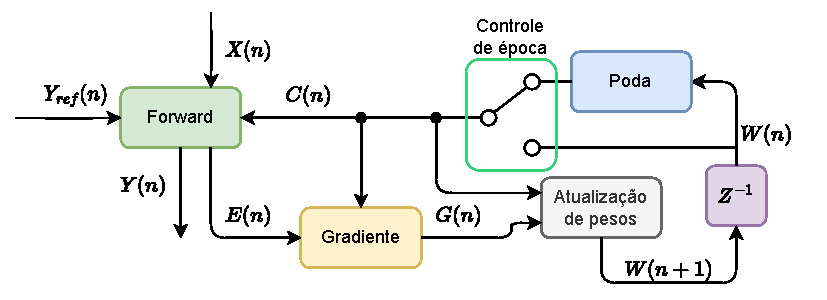
\includegraphics[width=0.7\textwidth]{figuras/prune_normal_scheme.pdf}
    \caption{Diagrama do loop de aprendizado utilizando poda com controle de época}
    \end{figure}
    As estratégias mais convencionais de poda realizam a remoção apenas uma vez por época. Geralmente no último mini-batch de cada época.
\end{frame}

\begin{frame}{Compressão consciente por poda}
    \begin{figure}[H]
    \centering
    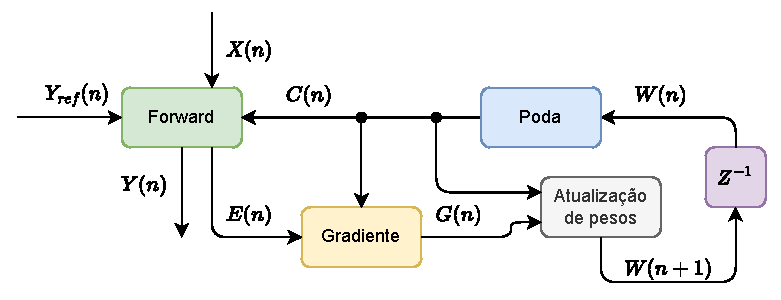
\includegraphics[width=0.7\textwidth]{figuras/prune_scheme.pdf}
    \caption{Diagrama do loop de aprendizado utilizando poda consciente a cada mini-batch}
    \end{figure}
    
\end{frame}

\begin{frame}{Compressão consciente por poda}
A estratégia utilizada para escolher quais pesos devem ser removidos é dada por 
\begin{equation}
    C_k(n) = P(W_k(n),\beta_k) =
    \begin{cases}
      w_k(n) & \text{if } |w_k(n)|\geq \beta_k \\
      0 & \text{if } |w_k(n)| < \beta_k\\
    \end{cases} ,
\end{equation}
onde $\beta_k$ é a janela de corte da $k$-ésima camada definida por
\begin{equation}
    \beta_k = \alpha \times \sigma_k,
\end{equation}
sendo $\sigma_k$ o desvio padrão da $k$-ésima camada e $\alpha$ o valor da agressividade da poda.

\end{frame}





\begin{frame}{Compressão consciente por poda}
    
\begin{figure}[H]
  \centering

  \begin{subfigure}[b]{0.49\textwidth}
    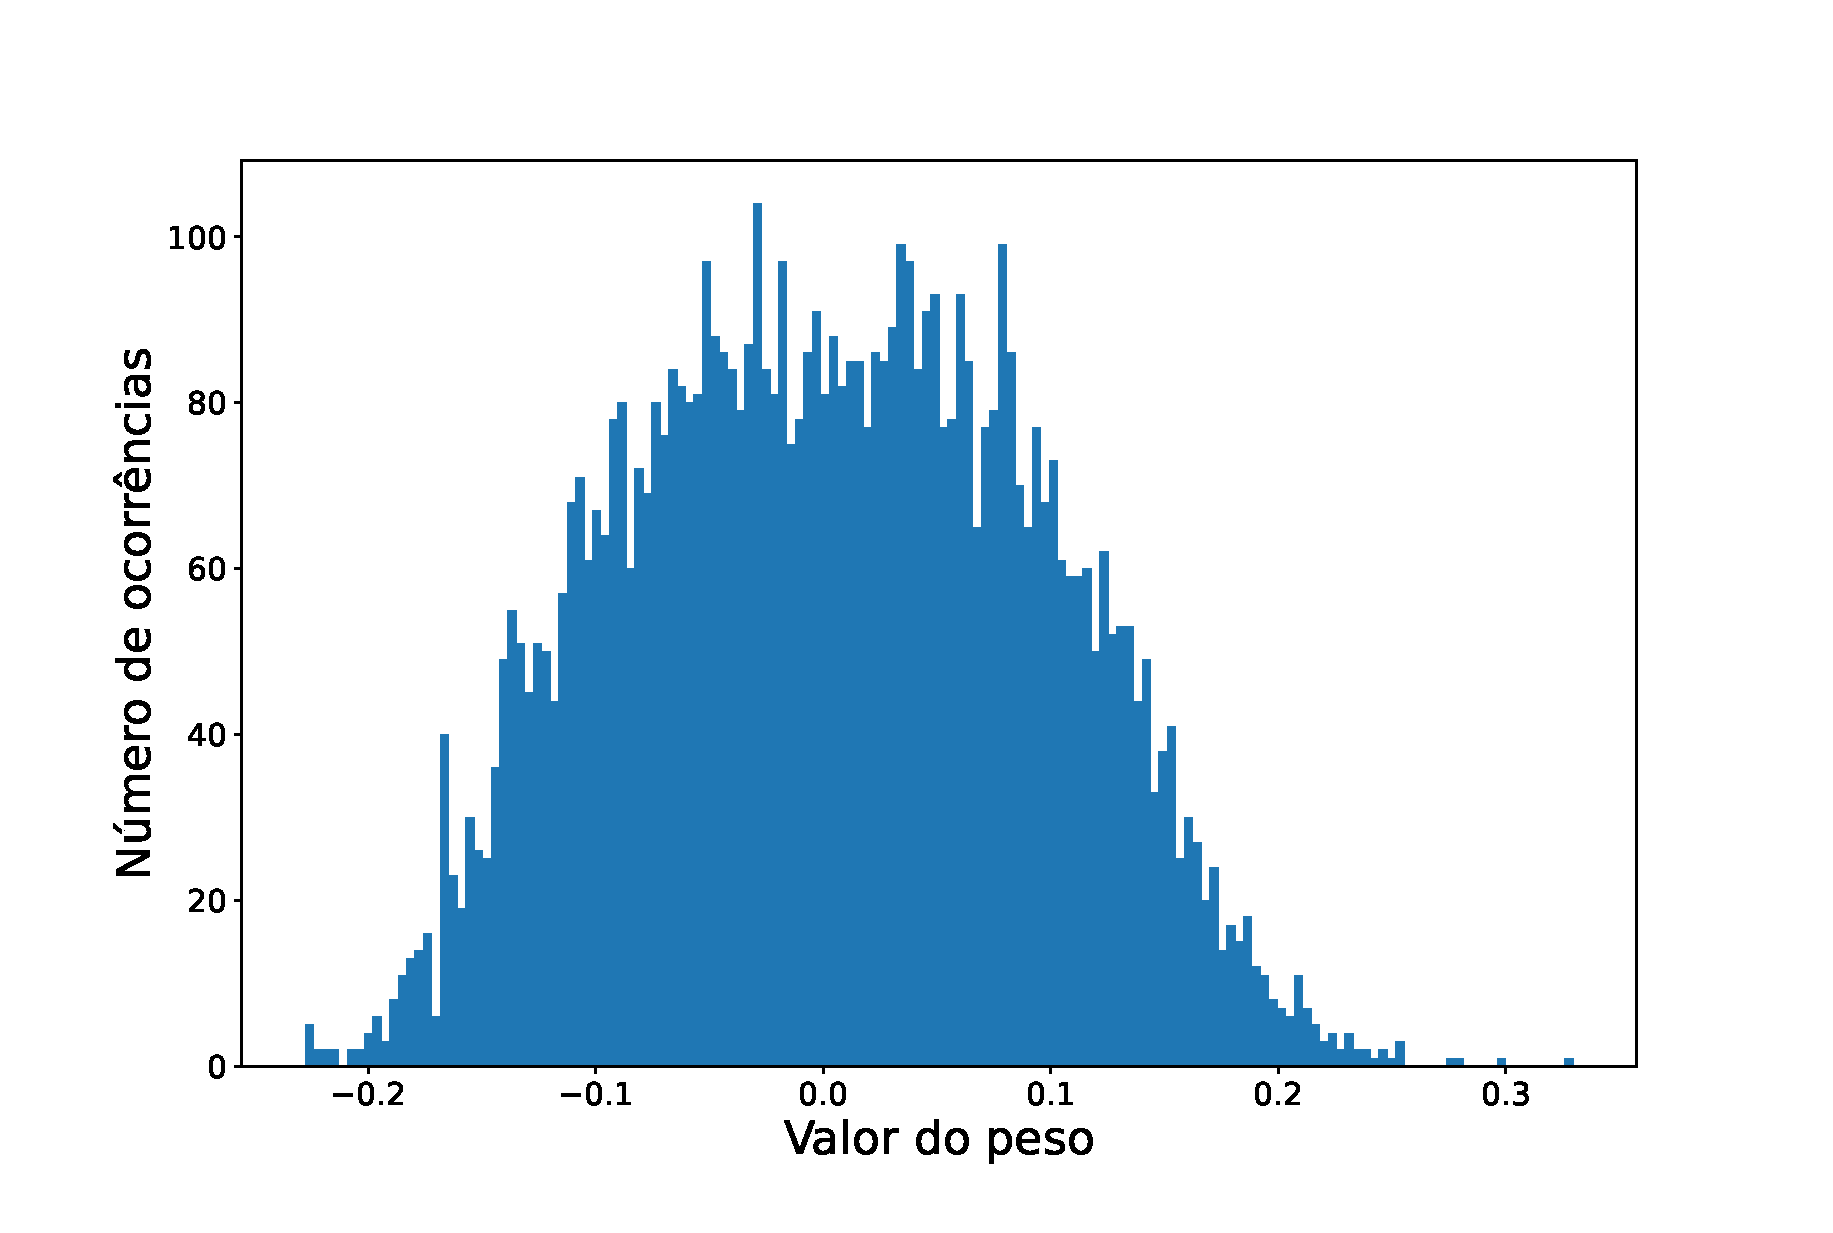
\includegraphics[width=\textwidth]{figuras/hist_weights.eps}
    \caption{Pesos não comprimidos}
    \label{fig:subfig1}
  \end{subfigure}
  \hfill
  \begin{subfigure}[b]{0.49\textwidth}
    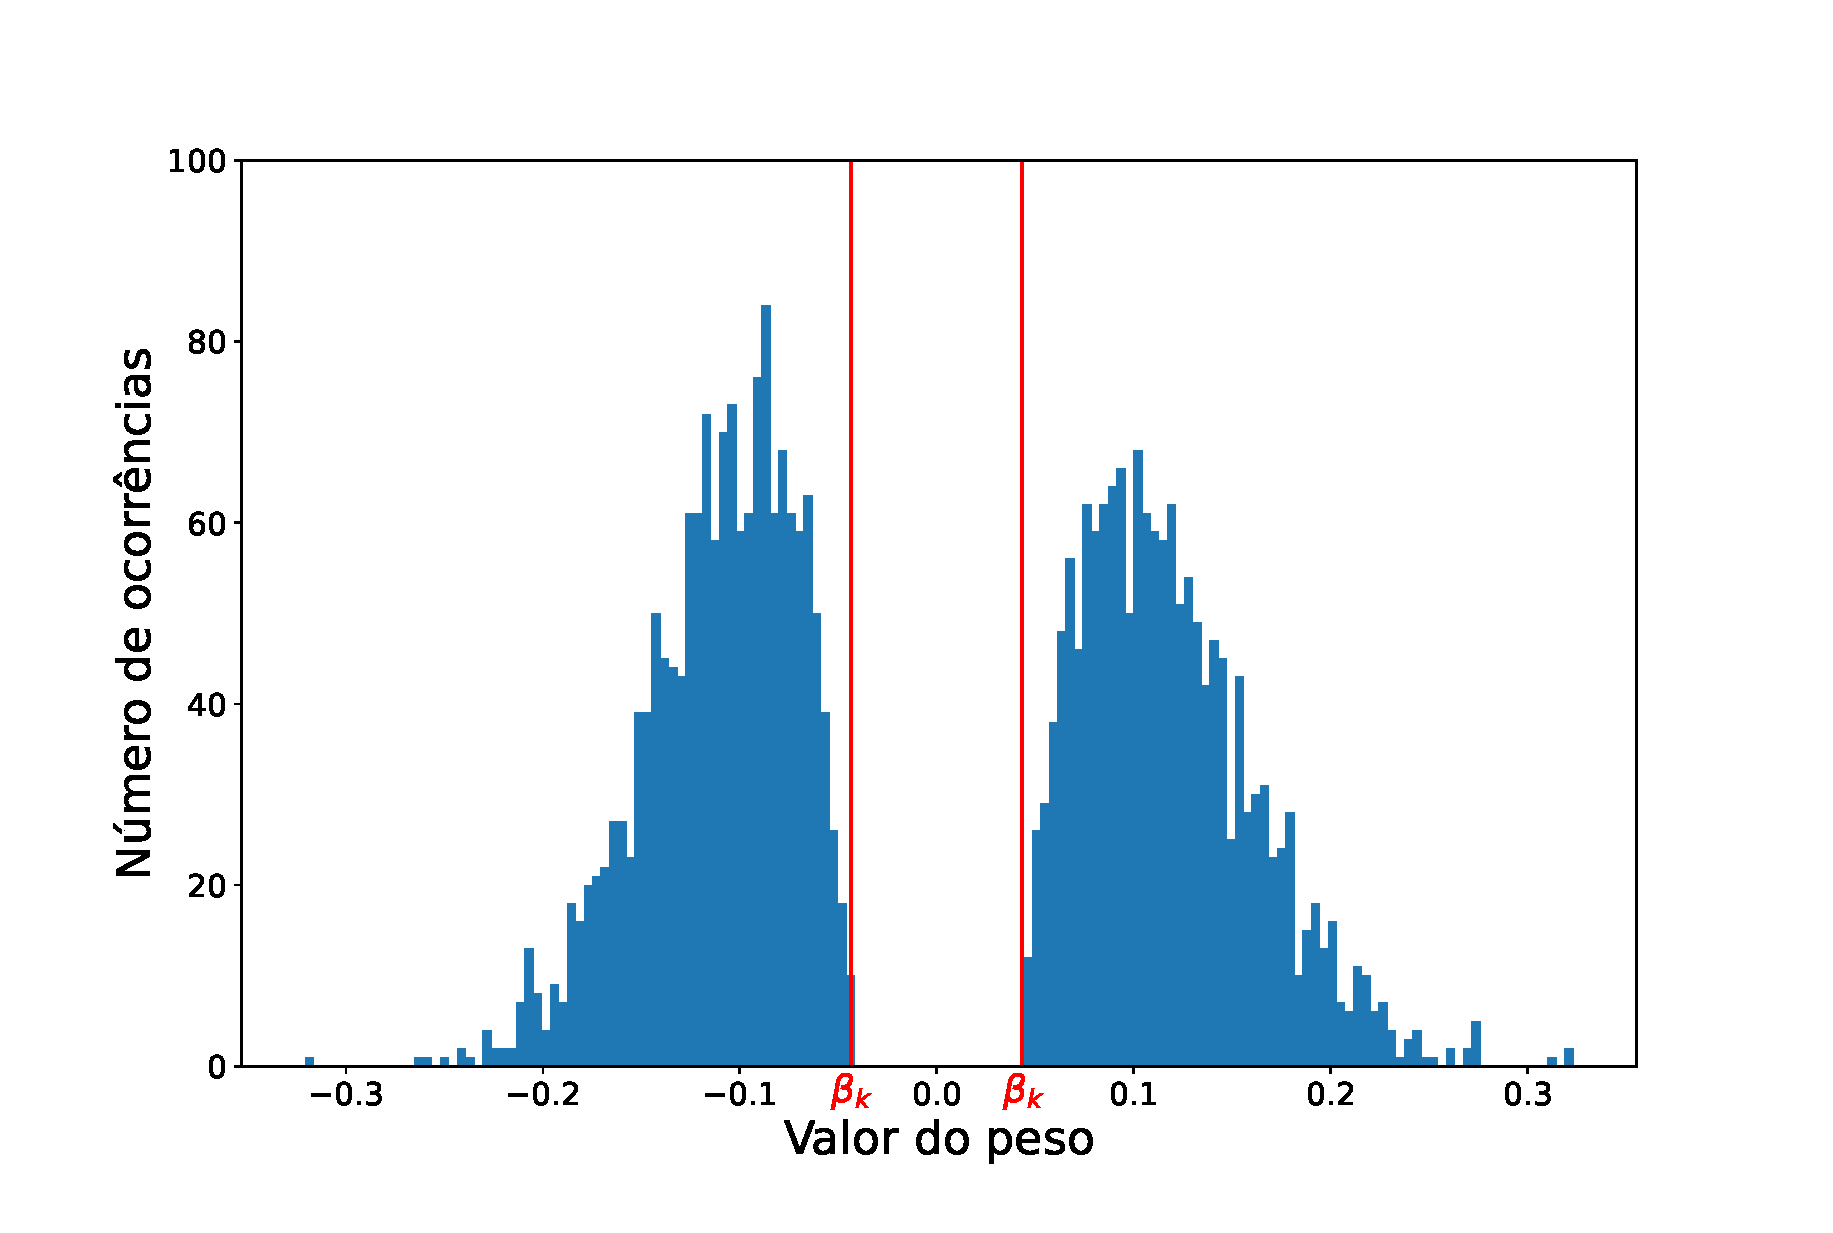
\includegraphics[width=\textwidth]{figuras/hist_prune.eps}
    \caption{Poda consciente}
    \label{fig:subfig2}
  \end{subfigure}

  \caption{Histograma do valores dos pesos associado a um exemplo de compressão de pesos por poda consciente com $\alpha=0,5$  ($\beta_k=0,5 \times \sigma_k$) aplicada à uma camada de uma rede CNN.}
  \label{fig:main}
\end{figure}

\end{frame}

\begin{frame}{Compressão consciente por Quantização}
    A quantização de DNNs é uma estratégia que visa reduzir o consumo de recursos computacionais nas operações matemáticas reduzindo a precisão dos parâmetros da rede diminuindo a representação, em bits, dos seus valores.
    
\end{frame}


\begin{frame}{Compressão consciente por Quantização}
    A estratégia utilizada para quantização de pesos é definida por 
\begin{equation}\label{EqQuantization}
    C_k(n) = Q\left (W_k(n) , q_k\right)= \left \lceil \frac{W_k(n)}{q_k} \right \rfloor \times q_k,
\end{equation}
    sendo $q_k$ definido como o fator de quantização, ou de escala, da $k$-ésima camada 
\begin{equation}
    q_k = \frac{\text{max} \left \{ \left | W_k(n) \right | \right \}}{2^{b-1}-1}.
    \label{ft_quant}
\end{equation}
    onde $b$ é o parâmetro que define a quantidade de bits para quantização.
\end{frame}

\begin{frame}{Compressão consciente por Quantização}
    \begin{figure}[H]
    \centering
    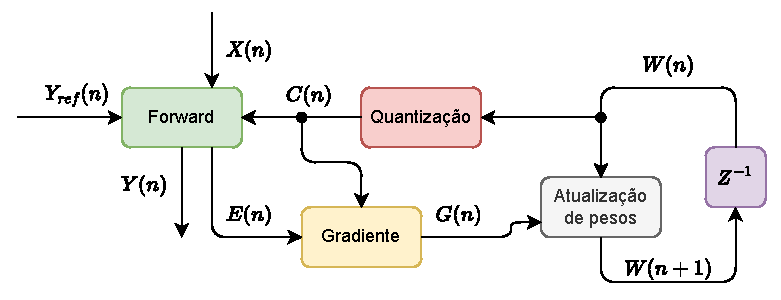
\includegraphics[width=0.7\textwidth]{figuras/quantization_scheme.pdf}
    \caption{Diagrama do loop de aprendizado com quantização}
    \end{figure}
\end{frame}

\begin{frame}{Compressão consciente por Quantização}
    \begin{figure}[H]
  \centering

  \begin{subfigure}[b]{0.49\textwidth}
    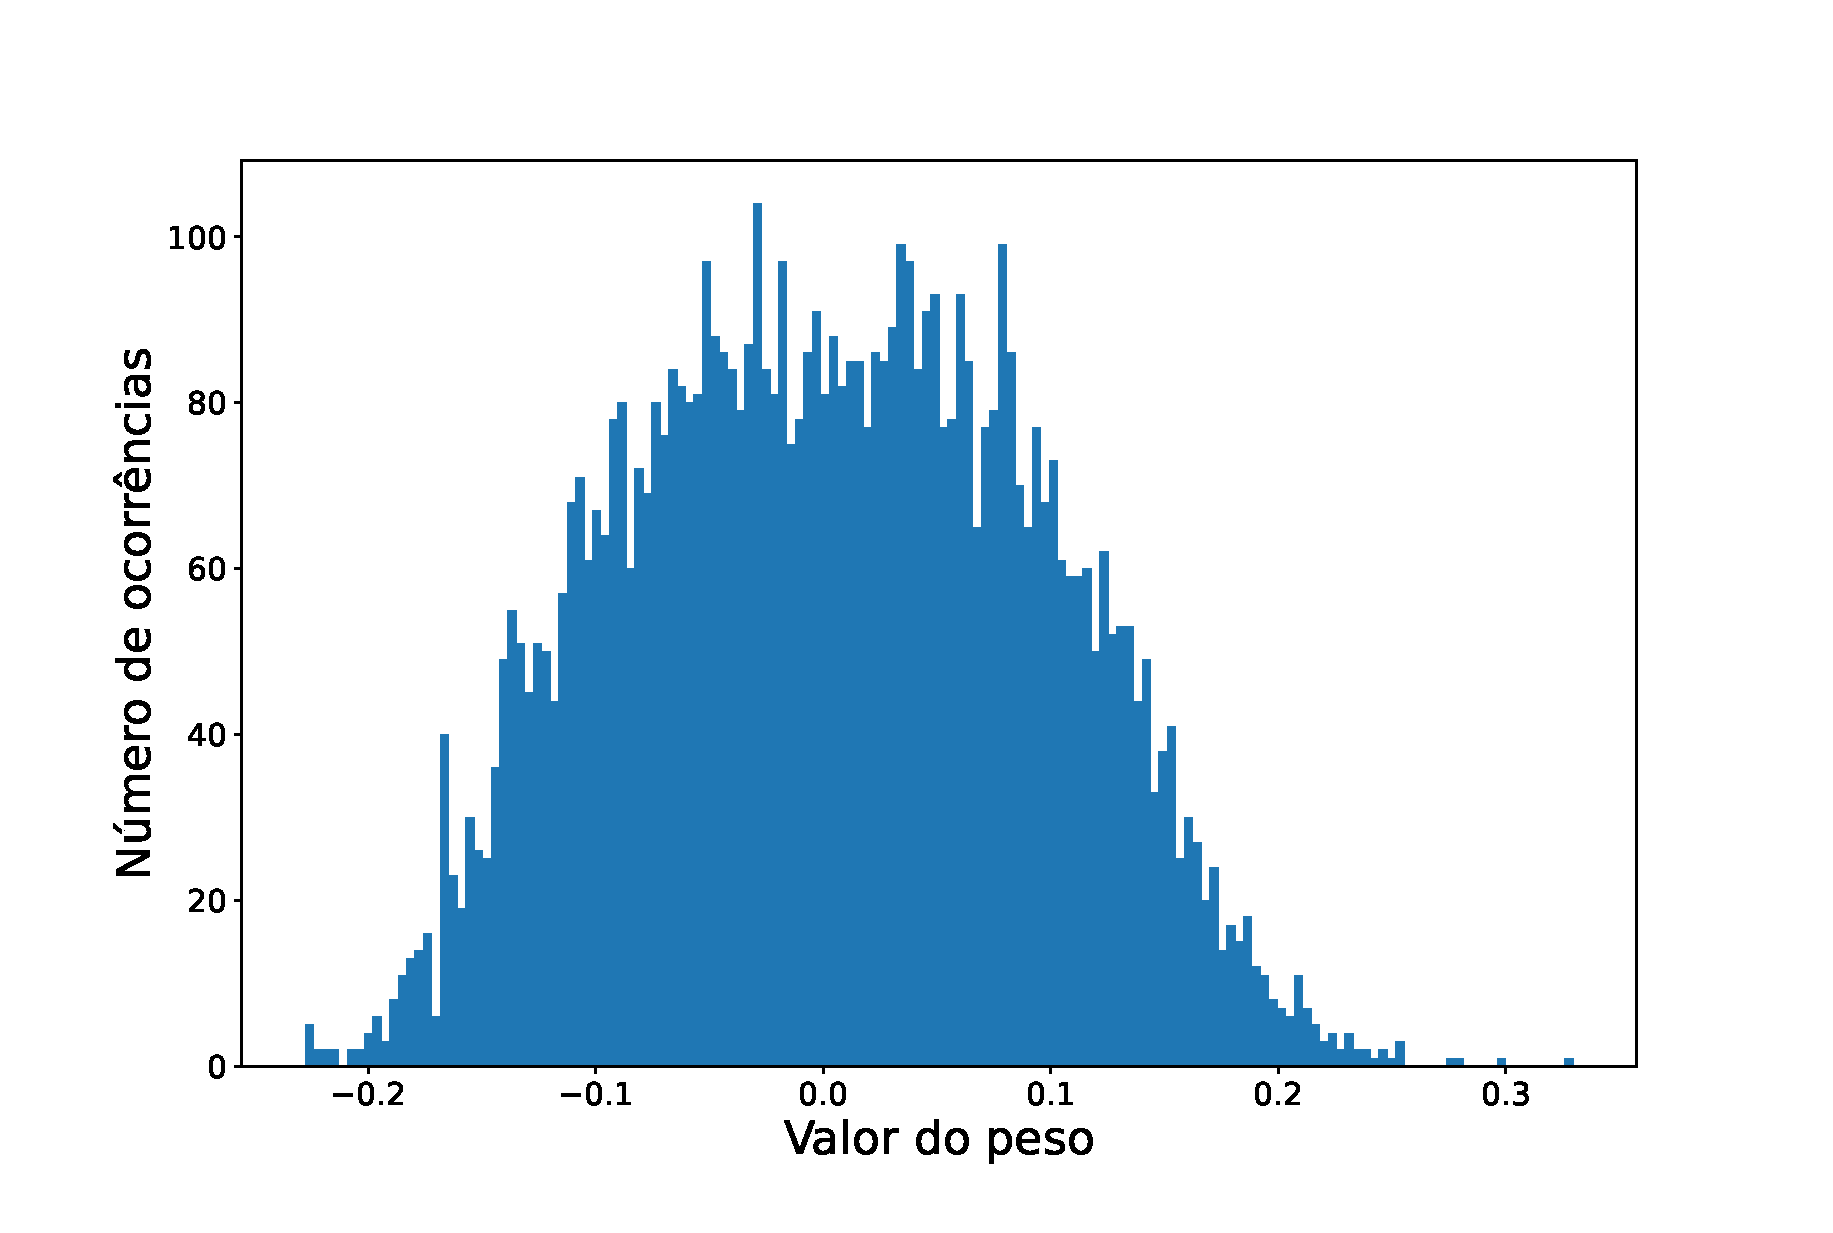
\includegraphics[width=\textwidth]{figuras/hist_weights.eps}
    \caption{Pesos não comprimidos}
    \label{fig:subfig1}
  \end{subfigure}
  \hfill
  \begin{subfigure}[b]{0.49\textwidth}
    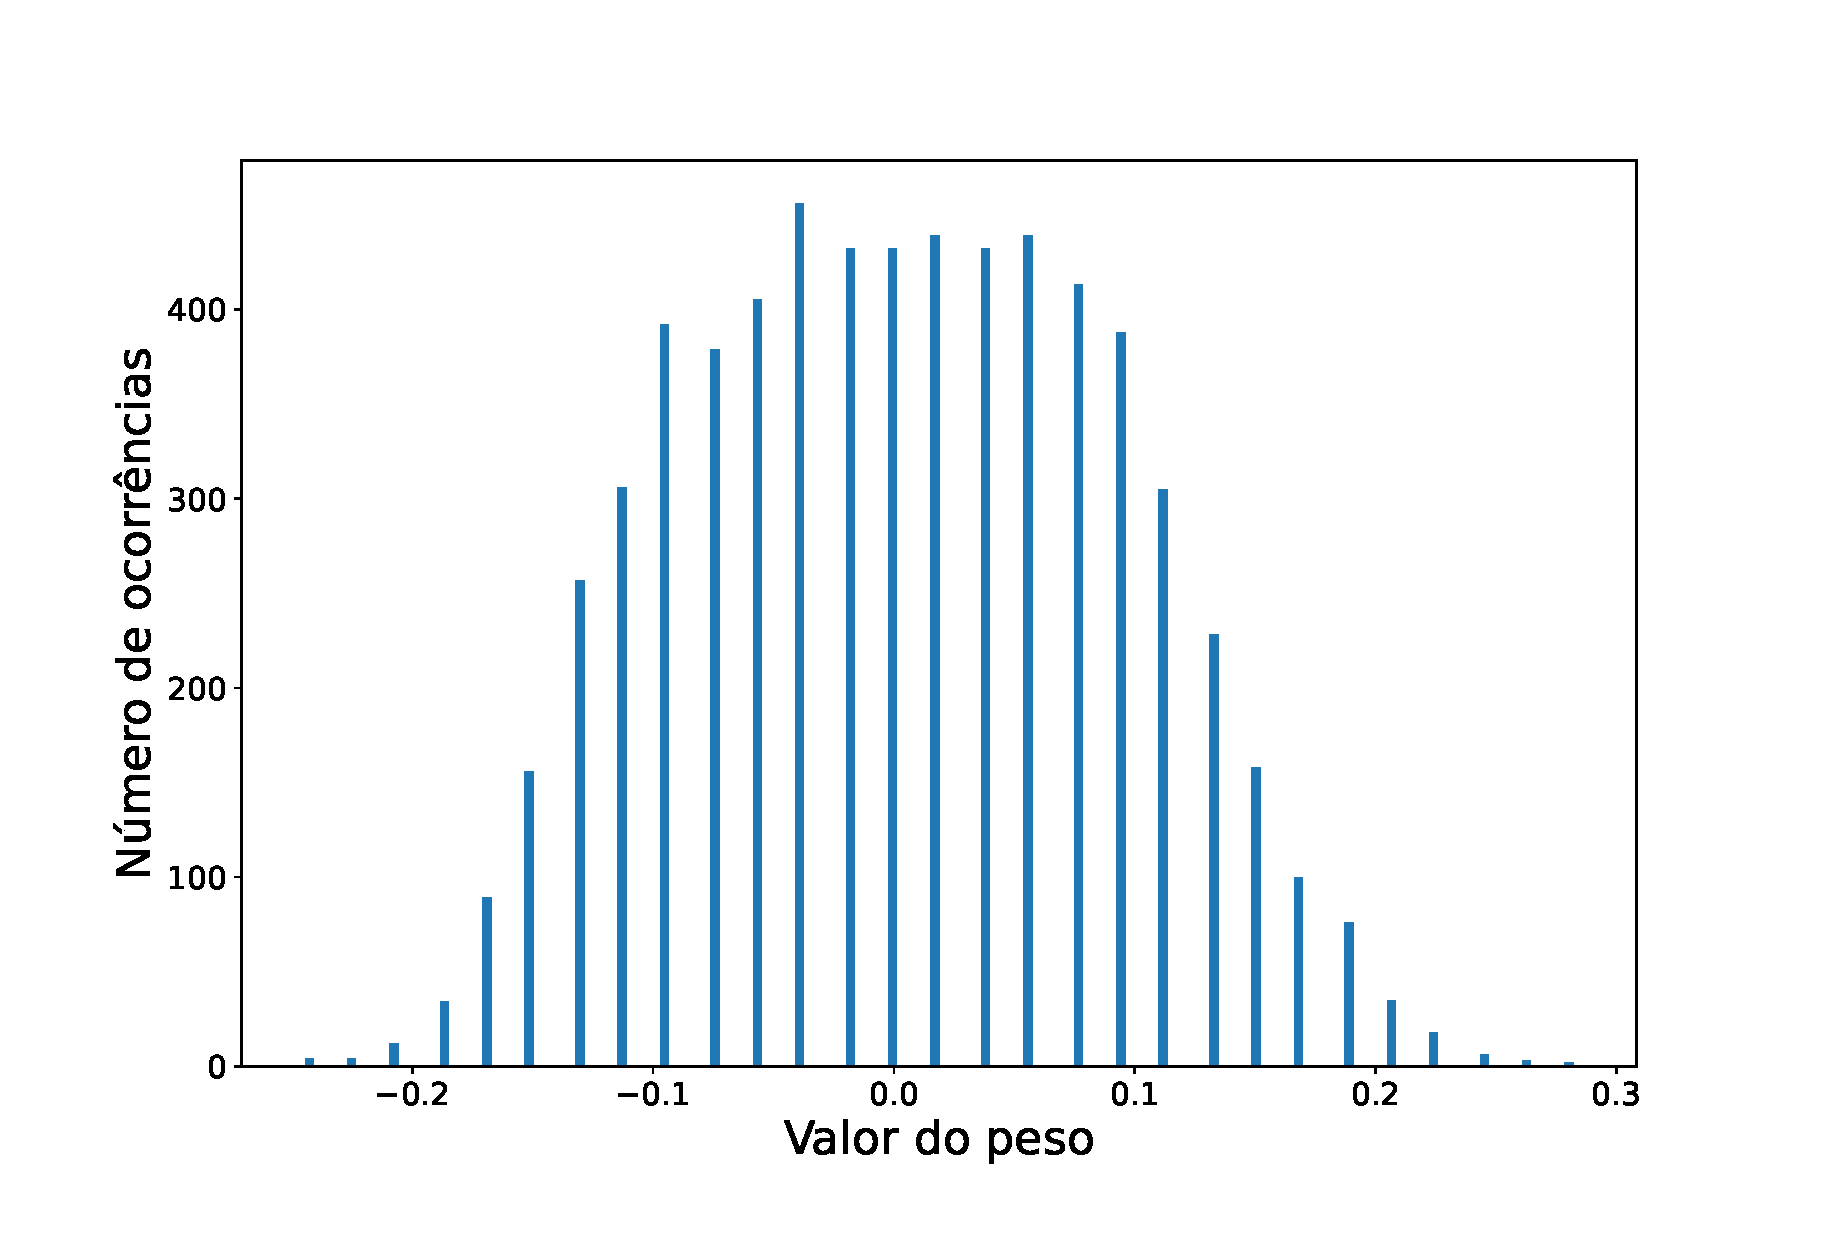
\includegraphics[width=\textwidth]{figuras/hist_quant.eps}
    \caption{Quantização consciente}
    \label{fig:subfig2}
  \end{subfigure}

  \caption{Histograma do valores dos pesos associado a um exemplo de compressão de pesos por quantização consciente com $b=5$ ($M=31$) aplicada à uma camada de uma rede CNN.}
  \label{fig:main}
\end{figure}
\end{frame}

\begin{frame}{Compressão consciente por Poda seguida de Quantização}
    Na compressão por poda seguida quantização, ambas as estratégias são utilizadas durante o treinamento, resultando na remoção de pesos insignificantes e quantização dos pesos remanescentes.
    
\end{frame}


\begin{frame}{Compressão consciente por Poda seguida de Quantização}
    A estratégia utilizada para poda seguida de quantização de pesos é definida por 
    \begin{equation}\label{EqPruningQuantization}
    C_k(n) = Q\left (  P \left ( W_k(n) , \beta_k \right ), q'_k \right),
    \end{equation}
    onde
    \begin{equation}
    q'_k = \frac{\text{max} \left \{ \left | W_k(n) \right | \right \} - \beta_k }{2^{b-1}-1}.
    \end{equation}.

\end{frame}

\begin{frame}{Compressão consciente por Poda seguida de Quantização}
    \begin{figure}[H]
    \centering
    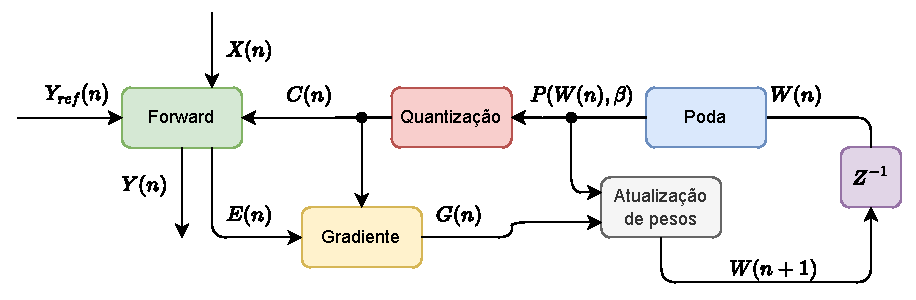
\includegraphics[width=0.7\textwidth]{figuras/prunequant_scheme.pdf}
    \caption{Diagrama do loop de aprendizado com poda seguida de quantização}
    \end{figure}
\end{frame}

\begin{frame}{Compressão consciente por Poda seguida de Quantização}
    \begin{figure}[H]
  \centering

  \begin{subfigure}[b]{0.49\textwidth}
    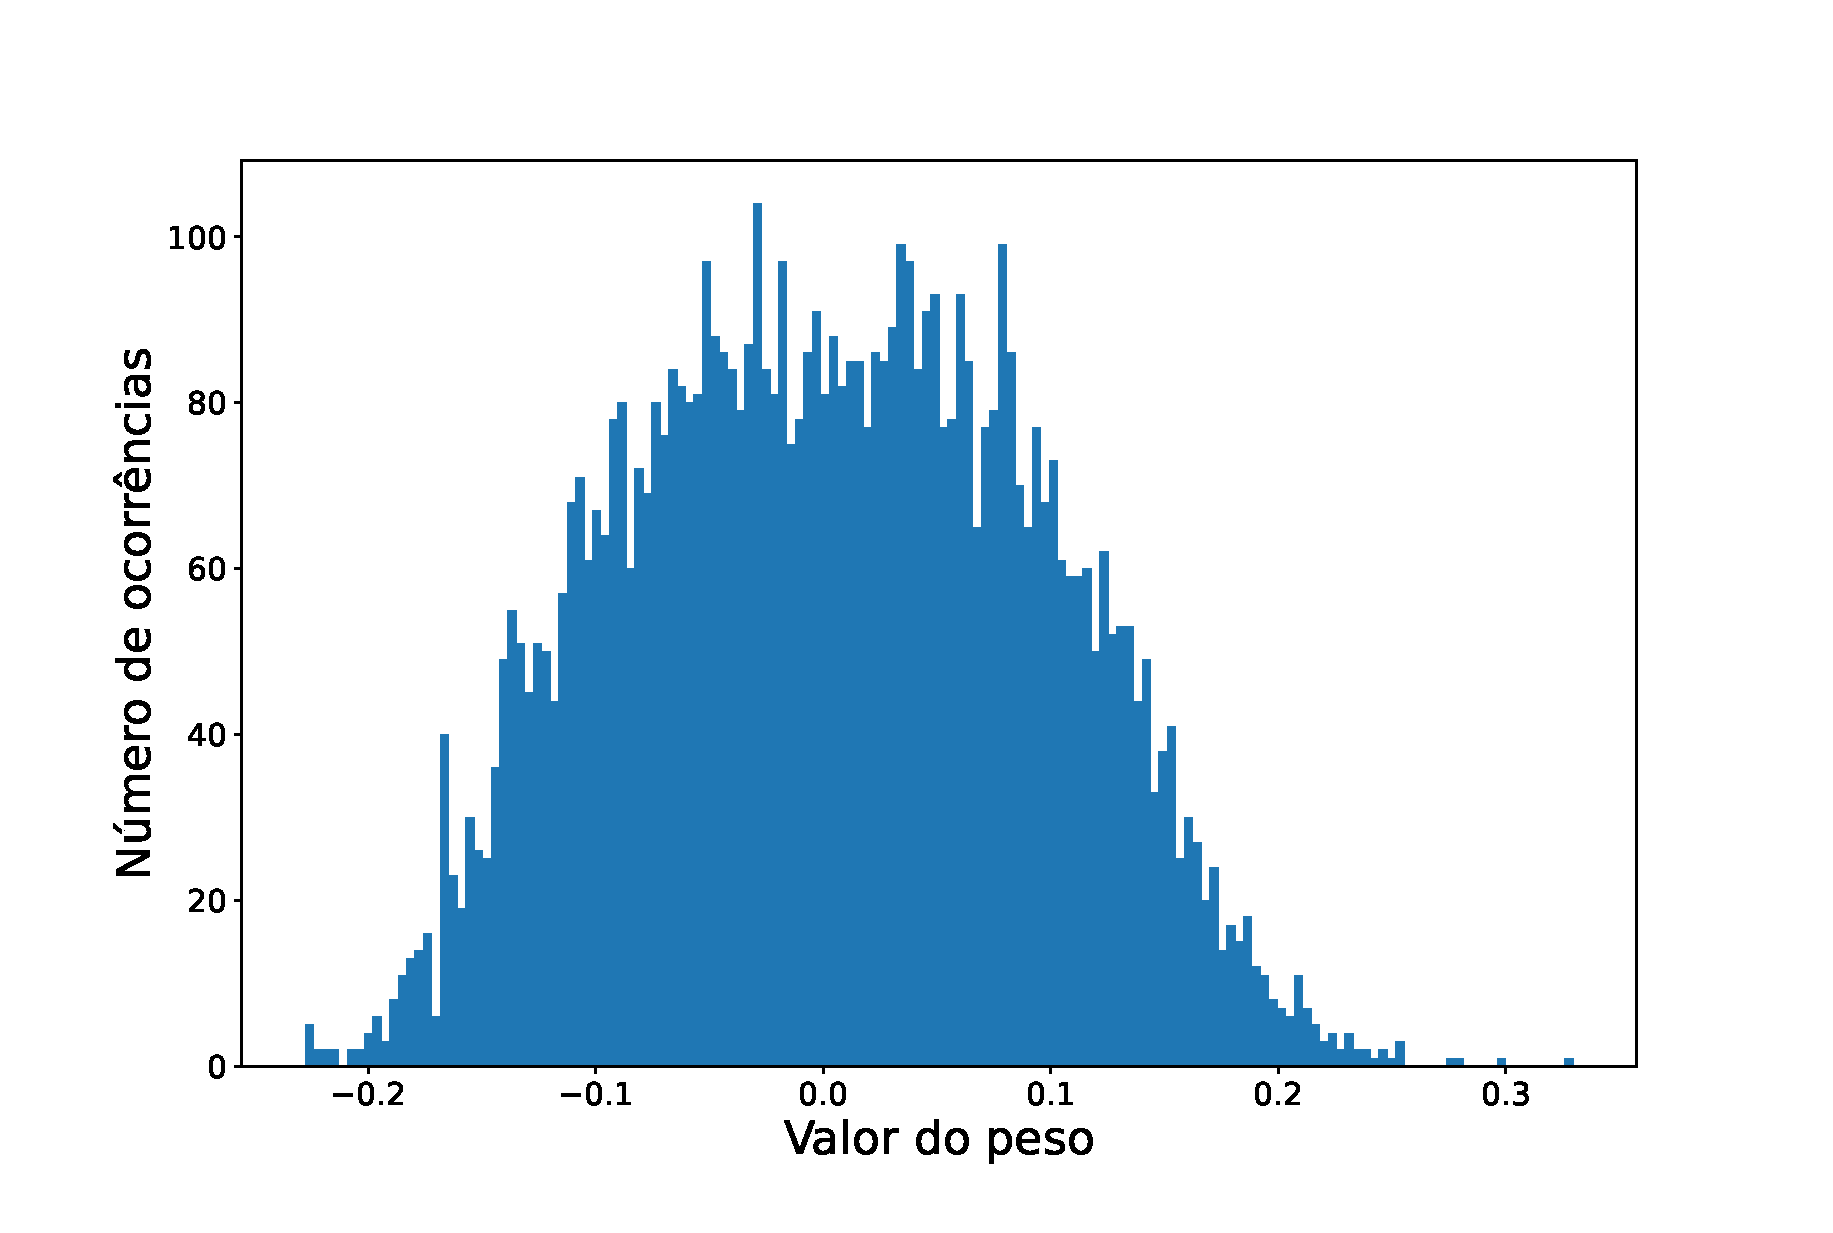
\includegraphics[width=\textwidth]{figuras/hist_weights.eps}
    \caption{Pesos não comprimidos}
    \label{fig:subfig1}
  \end{subfigure}
  \hfill
  \begin{subfigure}[b]{0.49\textwidth}
    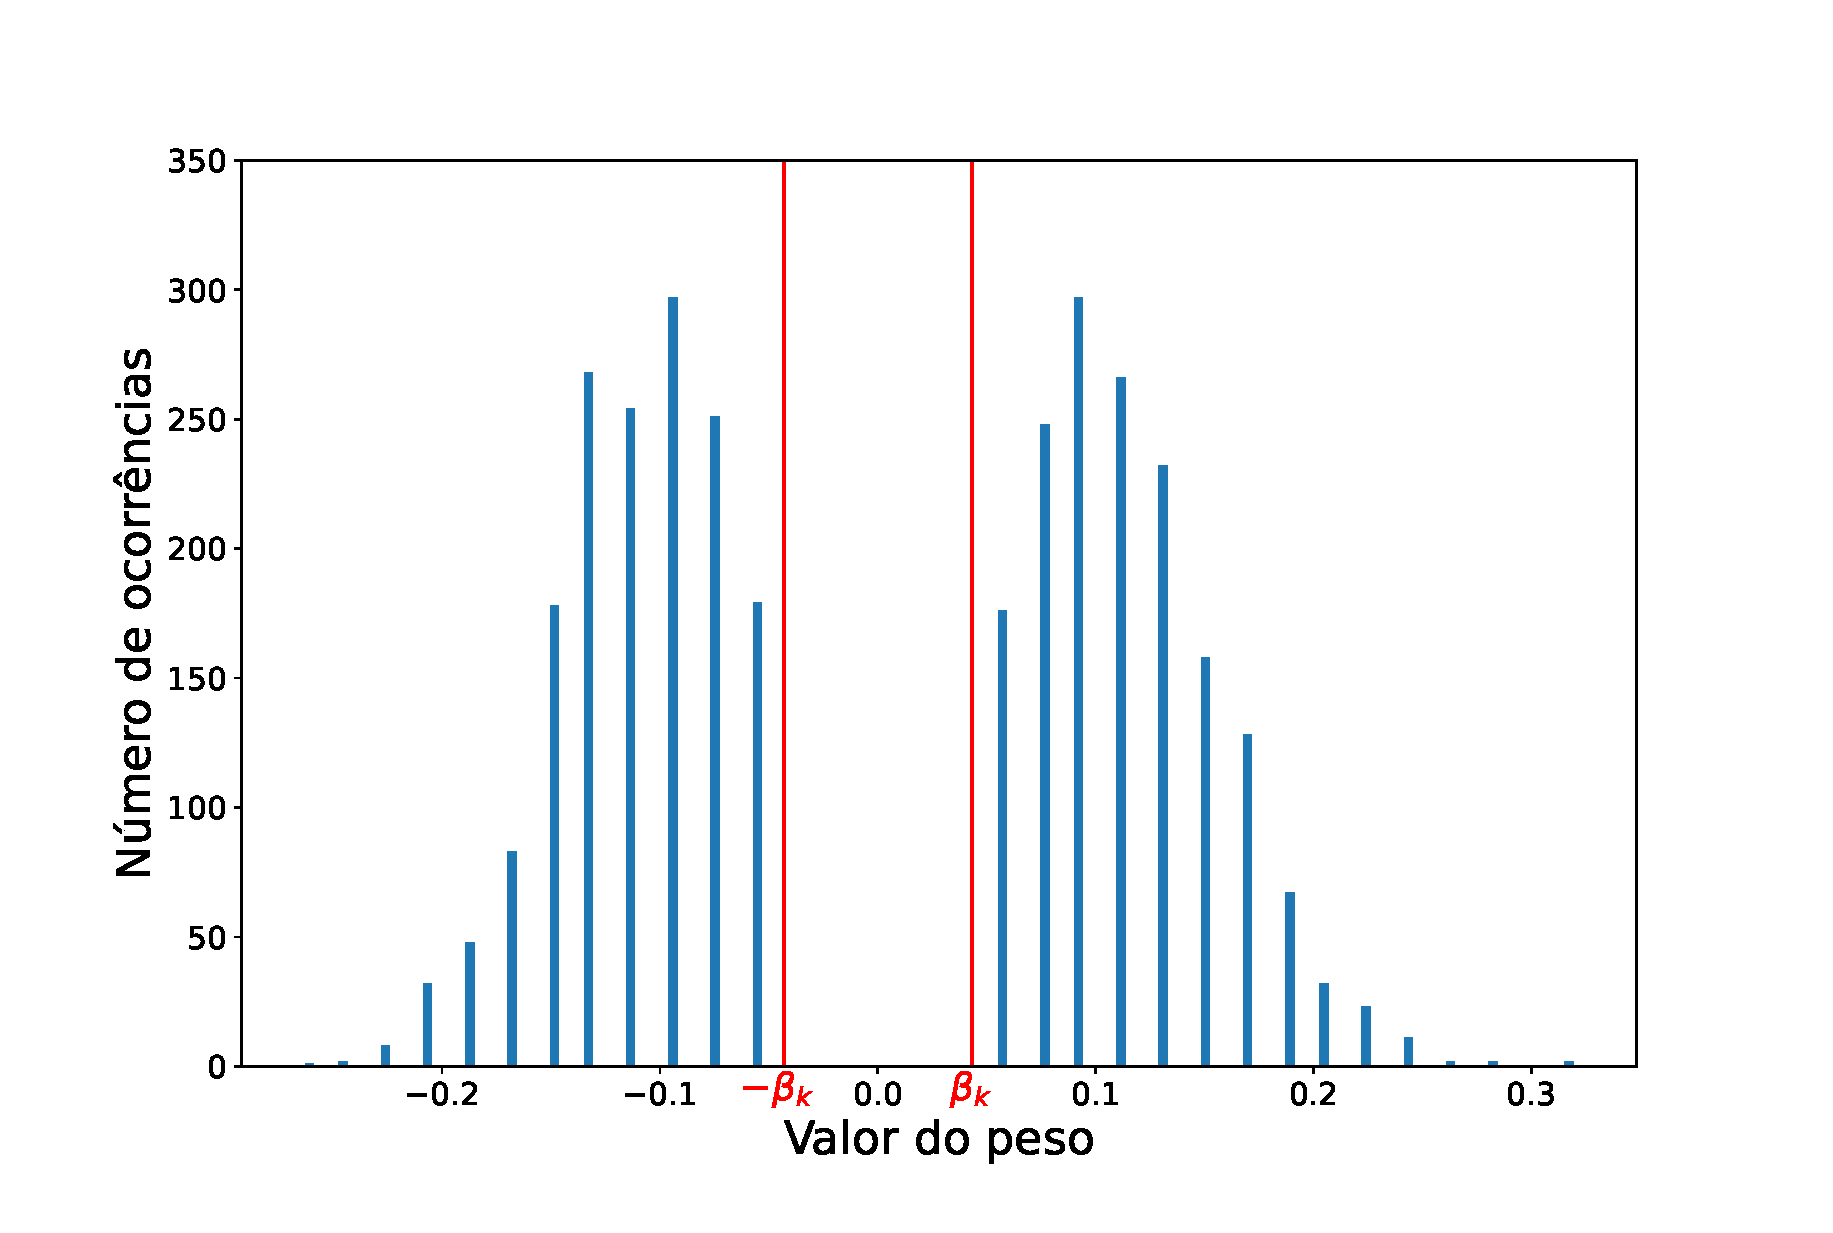
\includegraphics[width=\textwidth]{figuras/hist_prunequant.eps}
    \caption{Poda seguida de Quantização}
    \label{fig:subfig2}
  \end{subfigure}

  \caption{Histograma do valores dos pesos associado a um exemplo de compressão consciente dos pesos por poda seguida de quantização a cada iteração com $\alpha=0,5$ e $5$ bits aplicada à uma camada de uma rede CNN}
  \label{fig:main}
\end{figure}
\end{frame}

\begin{frame}{Geração de modelos comprimidos}
    Após utilização da técnica, o arquivo do modelo gerado precisa ser comprimido. A Para lidar com os modelos que sofreram a compressão por poda, é possível escolher duas estratégias:
    \begin{itemize}
        \item Gerar modelo no formato esparso:
        \begin{itemize}
            \item Modelo gerado salvo no formado esparso CSR ou CSC;
            \item Necessidade de hardwares específicos para operações esparsas;
            \item Modelos com baixa esparsidade podem aumentar o consumo de memória, tempo de inferência e processamento.
        \end{itemize}
        \item Manter formato denso e comprimir a partir de Deflate:
        \begin{itemize}
            \item O arquivo do modelo gerado é comprimido e menor que o original;
            \item Combina as técnicas de Huffman e Lempel-Ziv-Storer-Szymanski para compressão do modelo;
            \item A infererência é feita com o modelo no formato denso (pesos supostamente removidos).
        \end{itemize}
    \end{itemize}
\end{frame}

\begin{frame}
    Para a estratégia de quantização, os parâmetros do modelos são transformados para uma representação em bits, sendo calibrados a partir do fator de quantização $q_k$.
\end{frame}

% Metodologia
\section{Classificação de Modulações}

\begin{frame}{Classificação Automática de modulações}
    \begin{itemize}
        \item A Modulação, nas transmissões de dados, refere-se ao processo de modificar uma ou mais características de um sinal chamado de portadora para representar informações ou dados. 
        \item A modulação é necessária para transmitir dados por meio de um meio de comunicação, como cabos de cobre, fibras ópticas ou ondas de rádio.
        \item A classificação automática de modulação (\emph{automatic modulation classification} - AMC) é um problema clássico nas comunicações sem fio modernas. Um dos objetivos da AMC é entender e rotular o espectro de rádio em cenários de comunicação não cooperativos, o que facilita a detecção de falhas, monitoramento de interferência de espectro e acesso dinâmico ao espectro.
    \end{itemize}
\end{frame}

\begin{frame}{Dataset}
    O \emph{dataset} inclue efeitos de canal simulados sintéticamente e gravações pelo ar de $24$ tipos de modulação digital e analógica com as seguintes características:
    \begin{itemize}
        \item $26$ níveis de relação sinal ruído (SNR) ($-20$dB a $30$dB com passo de $2$dB);
        \item $2$ milhões de sinais;
        \item $4096$ realizações (frames) para cada par de modulação e SNR (2.555.904 frames no total);
        \item cada frame com $1024$ amostras In Phase e Quadrature (I/Q) ($2 \times 1024$).
    \end{itemize}
\end{frame}

\begin{frame}{Treinamento da DNN}
    Para o treinamento do modelo foram definidas as seguintes características:
    \begin{itemize}
        \item Tamanho de cada batch de $64$;
        \item Otimizador de Descida de Gradiente Estocástico (SGD);
        \item $70\%$ das amostras para treinamento e $30\%$ para validação;
        \item Taxa de aprendizagem de $0,05$ e momento de $0,9$;
        \item Critério de loss como entropia cruzada de categoria.
    \end{itemize}
\end{frame}

\begin{frame}{Arquitetura do modelo}
O modelo foi criado com a seguinte arquitetura:
\begin{minipage}[t]{0.45\textwidth}
\begin{itemize}
  \item Entrada ($1024 \times 2$);
        \item Bloco repetido $6$ vezes:
        \begin{itemize}
            \item Conv1D ($40 \times 4$);
            \item BatchNorm;
            \item ReLU;
            \item MaxPool ($2$);
        \end{itemize}
        \item Flatten;
        \item Dense($128$);
        \item BatchNorm;
        \item ReLU;
\end{itemize}
\end{minipage}
\hfill
\begin{minipage}[t]{0.45\textwidth}
\begin{itemize}
  \item Dense($128$);
  \item BatchNorm;
  \item ReLU;
  \item Dense($7$);
  \item Softmax;
\end{itemize}
\end{minipage}
\end{frame}


\begin{frame}{Resultados}
    \begin{table}[H]
    \caption{Acurácias obtidas a partir do modelo comprimido para vários valores de tamanho de bits e $\alpha$.}
    \label{tab_acc}
    \centering
    \begin{tabular}{l|lllll}
    \hline
    \textbf{\diagbox{$\alpha$}{bits}} & \textbf{32 bits}  & \textbf{16 bits} & \textbf{8 bits} & \textbf{4 bits} & \textbf{3 bits}\\ \hline
    \textbf{0,00} &	97,06\%	& 96,93\%	& 97,00\% & 84,18\%	& 83,89\%\\
    \textbf{0,25} &	96,13\%	& 96,68\%	& 95,77\% & 92,03\%	& 84,00\%\\
    \textbf{0,50} &	96,70\%	& 96,41\%	& 96,43\% & 84,31\%	& 83,41\%\\
    \textbf{0,75} & 94,46\%	& 95,20\%  & 95,18\% & 90,55\%	& 83,36\%\\\hline
    \end{tabular}
\end{table}
\end{frame}

\begin{frame}{Resultados}
    \begin{table}[H]
    \caption{Valores de esparsidade obtidos a partir do modelo comprimido para vários valores de tamanho de bits e $\alpha$.}
    \label{tab_spa}
    \centering
    \begin{tabular}{l|lllll}
    \hline
    \textbf{\diagbox{$\alpha$}{bits}} & \textbf{32 bits}  & \textbf{16 bits} & \textbf{8 bits} & \textbf{4 bits} & \textbf{3 bits}\\ \hline
    \textbf{0,25} &	42,17\%	& 47,31\%	& 48,11\% & 45,85\%	& 38,50\%\\
    \textbf{0,50} &	66,26\%	& 60,82\%	& 61,28\% & 60,61\%	& 41,60\%\\
    \textbf{0,75} & 74,78\%	& 69,75\%  & 76,11\% & 68,41\%	& 62,44\%\\\hline
    \end{tabular}
\end{table}
\end{frame}

\begin{frame}{Resultados}
    \begin{table}[H]
    \caption{Tamanho do modelo comprimido para vários valores de tamanho de bits e $\alpha$.}
    \label{tab_siz}
    \centering
    \begin{tabular}{l|lllll}
    \hline
    \textbf{\diagbox{$\alpha$}{bits}} & \textbf{32 bits}  & \textbf{16 bits} & \textbf{8 bits} & \textbf{4 bits} & \textbf{3 bits}\\ \hline
    \textbf{0,00} &	3,18Mb	& 1,59Mb	& 0,80Mb & 0,40Mb	& 0,30Mb\\
    \textbf{0,25} &	1,84Mb	& 0,84Mb	& 0,41Mb & 0,26Mb	& 0,18Mb\\
    \textbf{0,50} &	1,08Mb	& 0,62Mb	& 0,31Mb & 0,16Mb	& 0,17Mb\\
    \textbf{0,75} & 0,80Mb	& 0,48Mb  & 0,19Mb & 0,13Mb	& 0,11Mb\\\hline
    \end{tabular}
\end{table}
\end{frame}


\begin{frame}{Resultados}
    \begin{figure}[H]
    \centering
    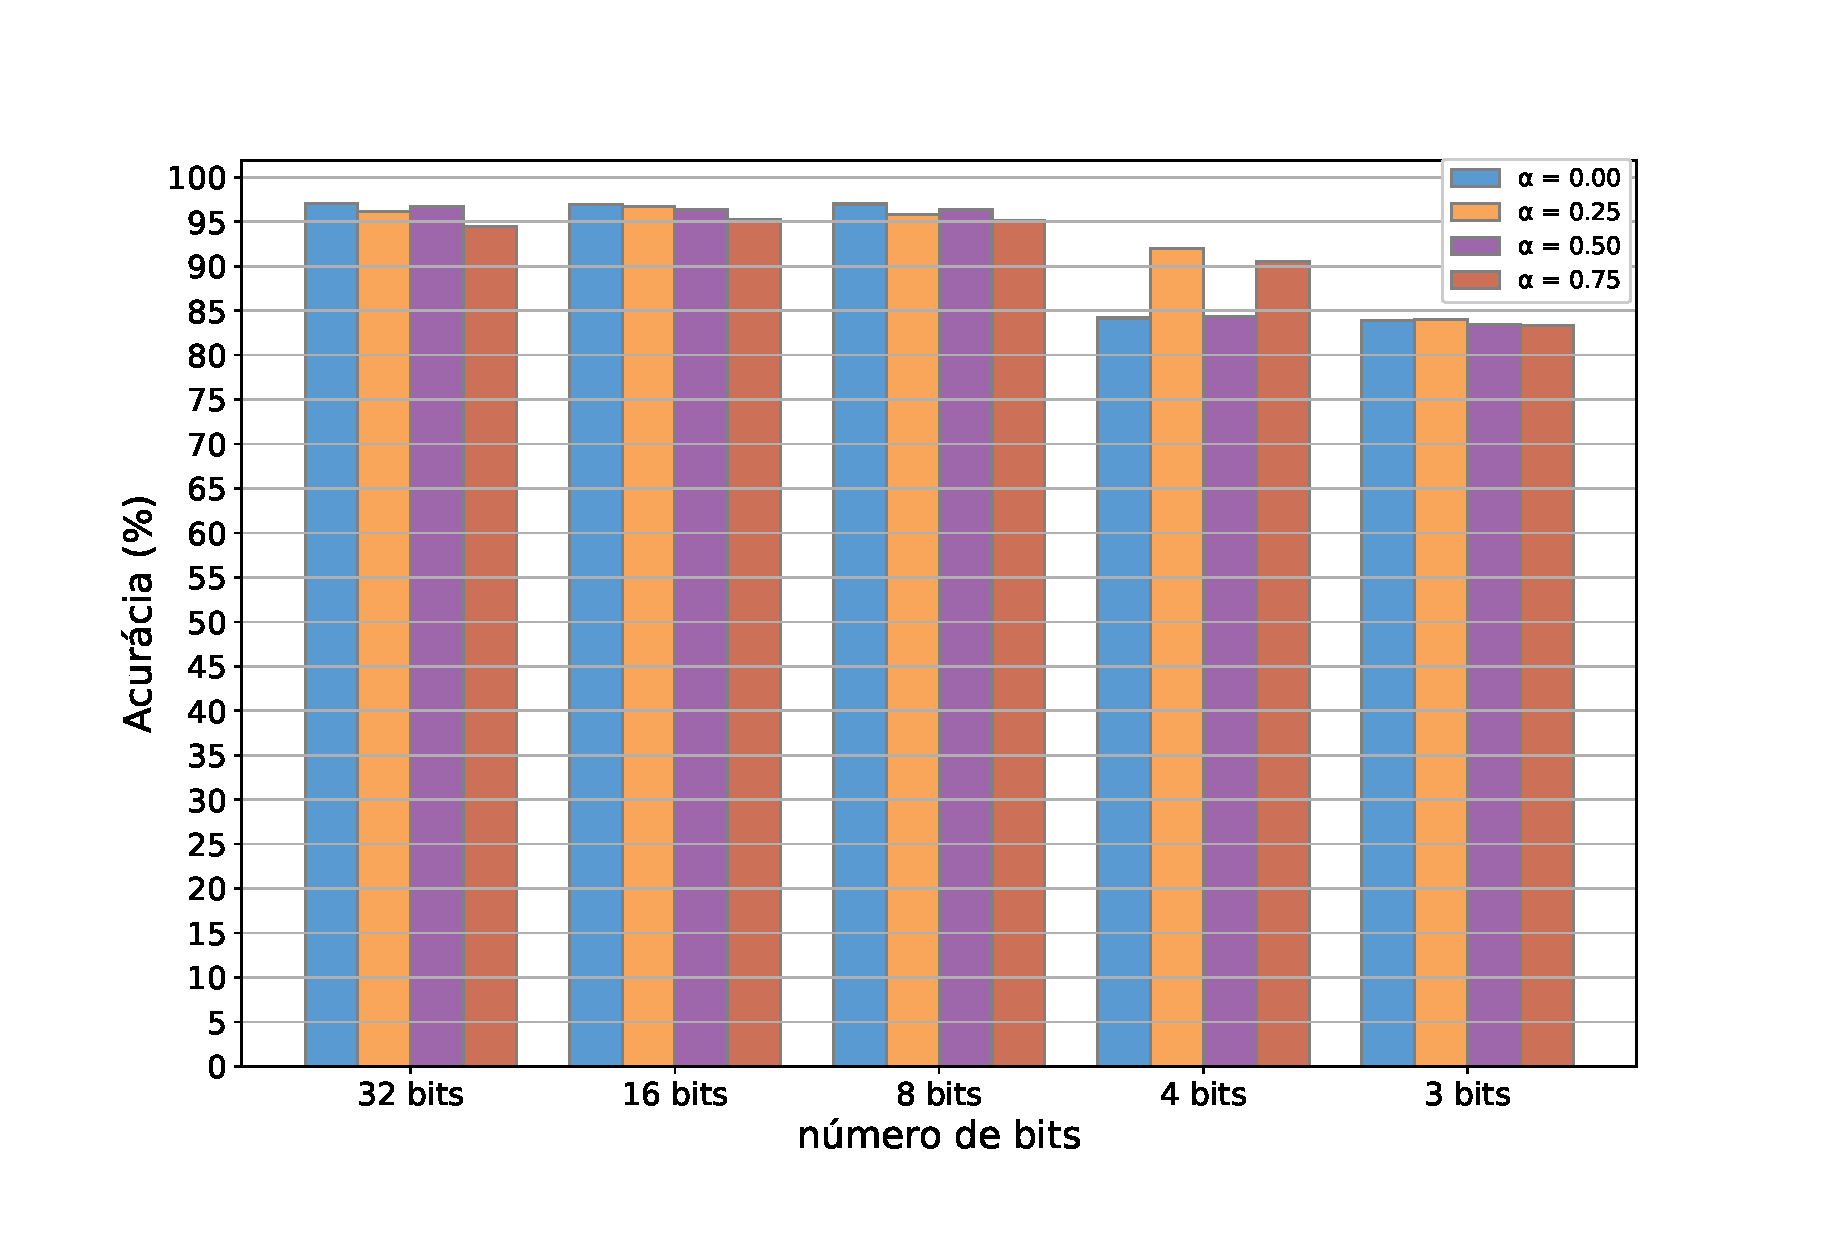
\includegraphics[width=0.7\textwidth]{figuras/accuracies.eps}
    \caption{Acurácias obtidas para diversas configuração de $\alpha$ e número de bits}
    \end{figure}
\end{frame}

\begin{frame}{Resultados}
    \begin{figure}[H]
    \centering
    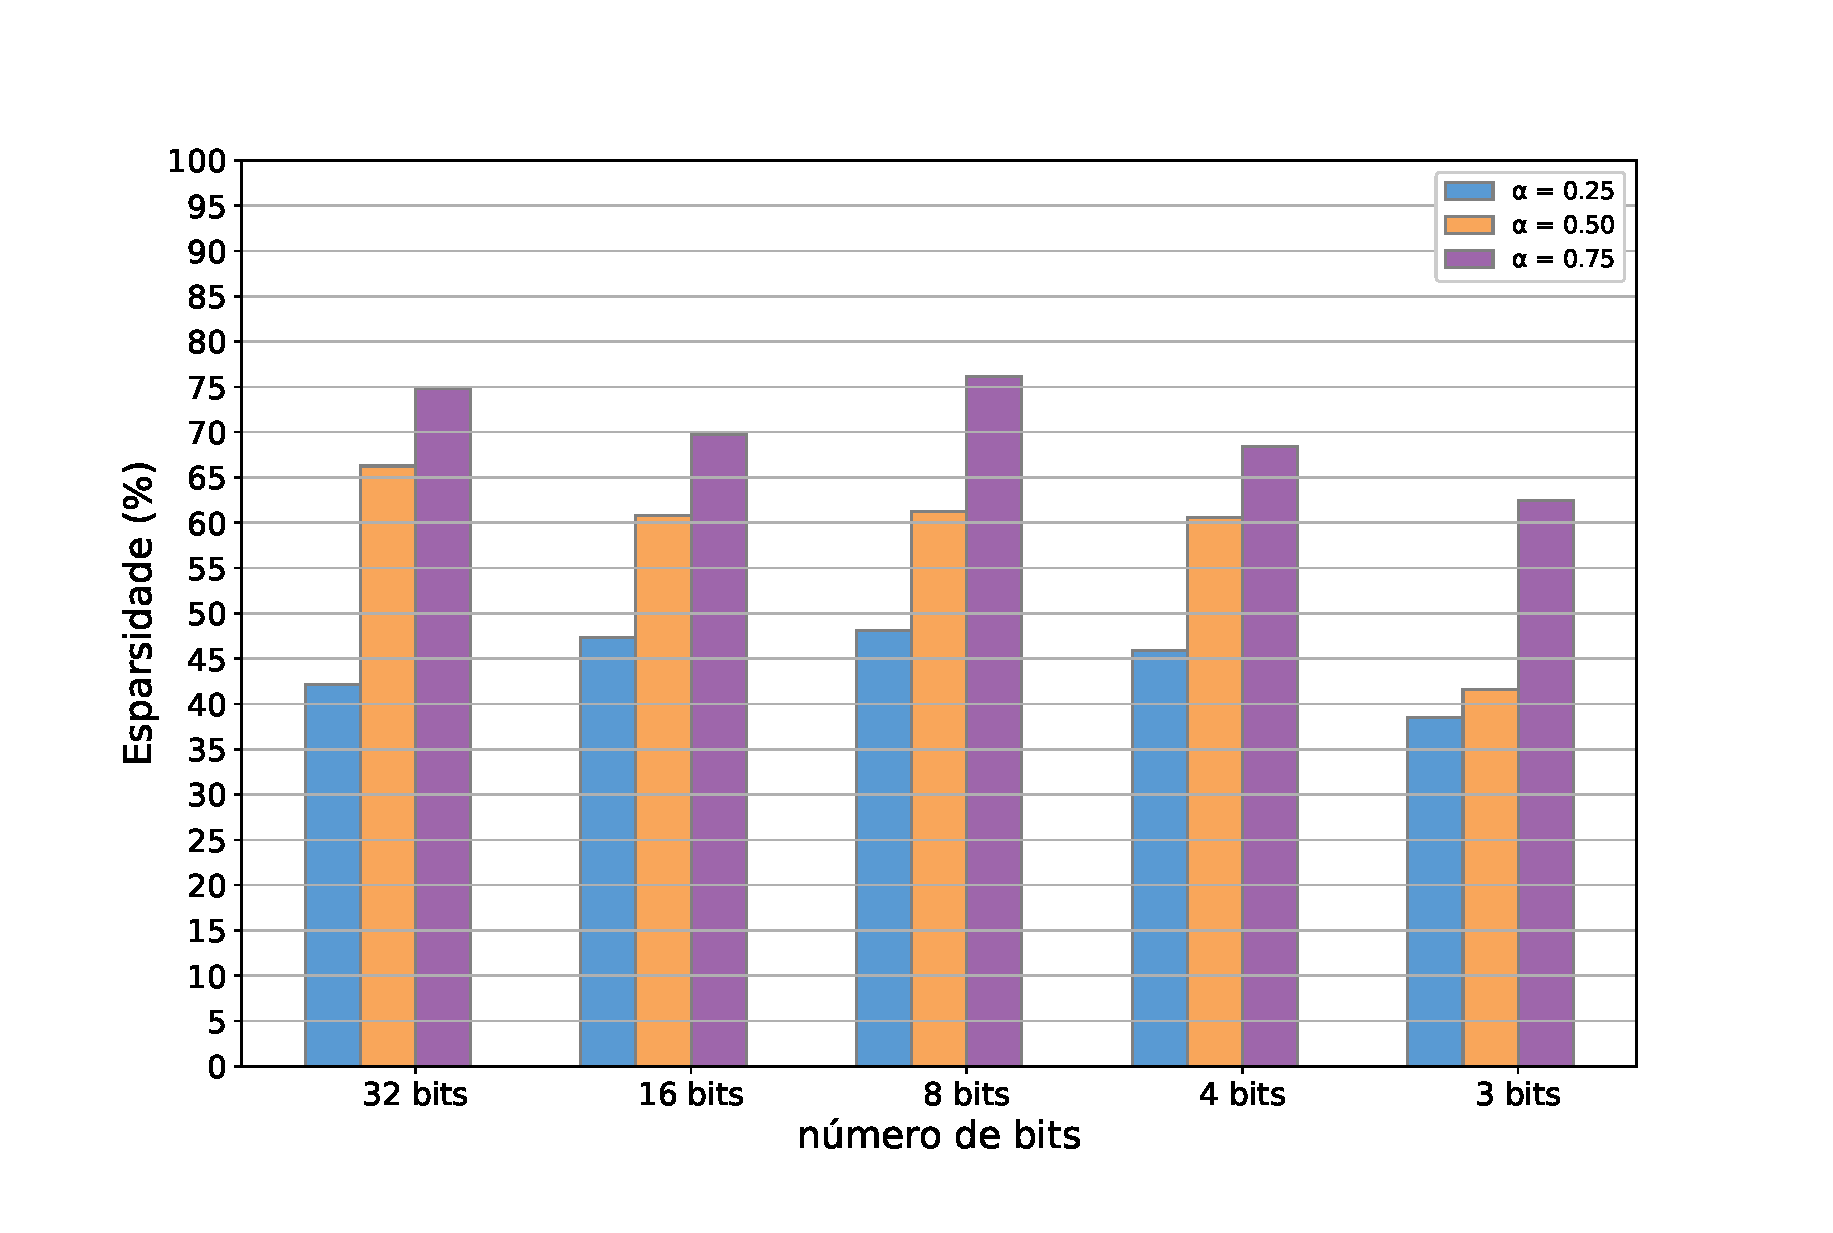
\includegraphics[width=0.7\textwidth]{figuras/sparsity.eps}
    \caption{Esparsidades obtidas para diversas configuração de $\alpha$ e número de bits}
    \end{figure}
\end{frame}

\begin{frame}{Resultados}
    \begin{figure}[H]
    \centering
    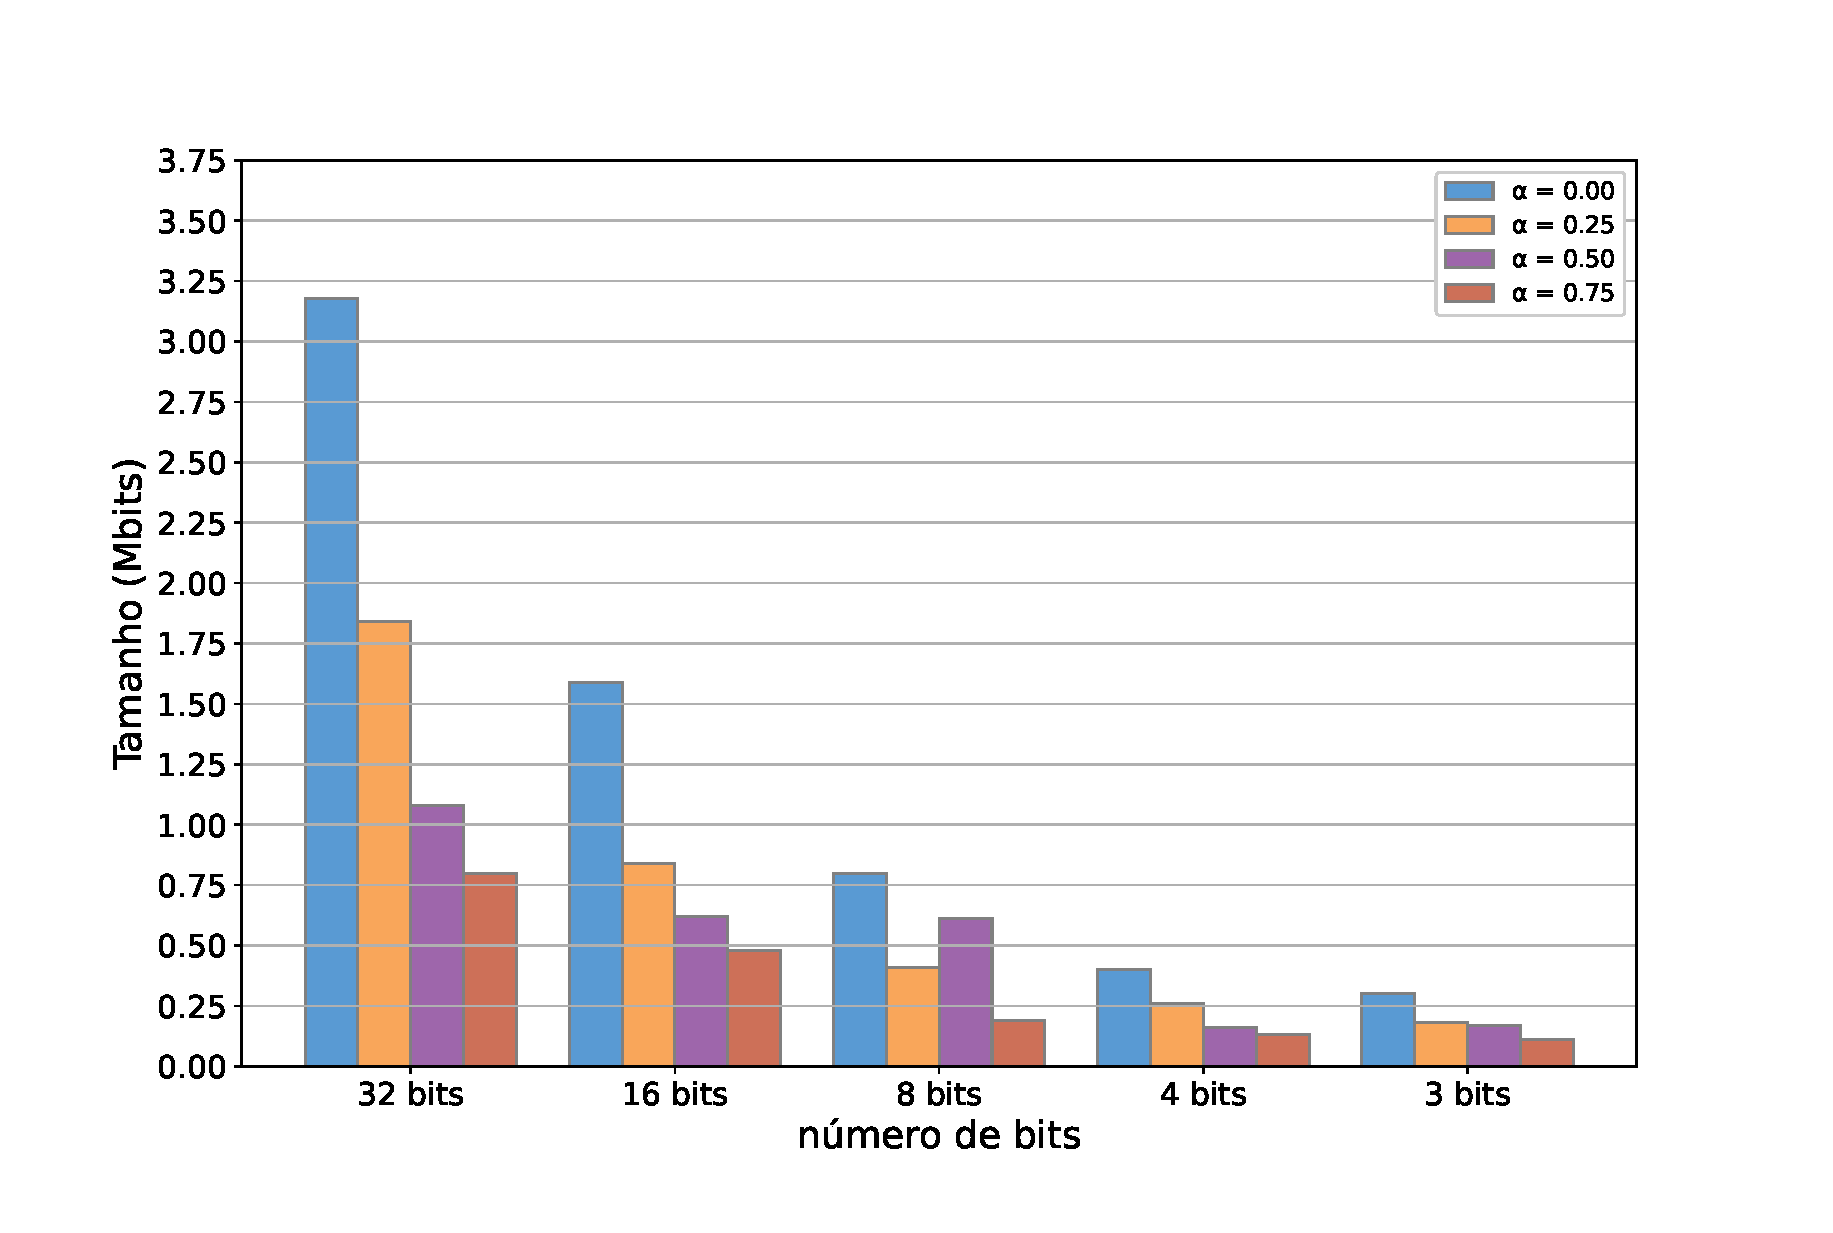
\includegraphics[width=0.7\textwidth]{figuras/sizes.eps}
    \caption{Tamanhos dos modelos obtidos para diversas configuração de $\alpha$ e número de bits}
    \end{figure}
\end{frame}

\begin{frame}{Resultados}
    \begin{figure}[H]
  \centering

  \begin{subfigure}[b]{0.45\textwidth}
    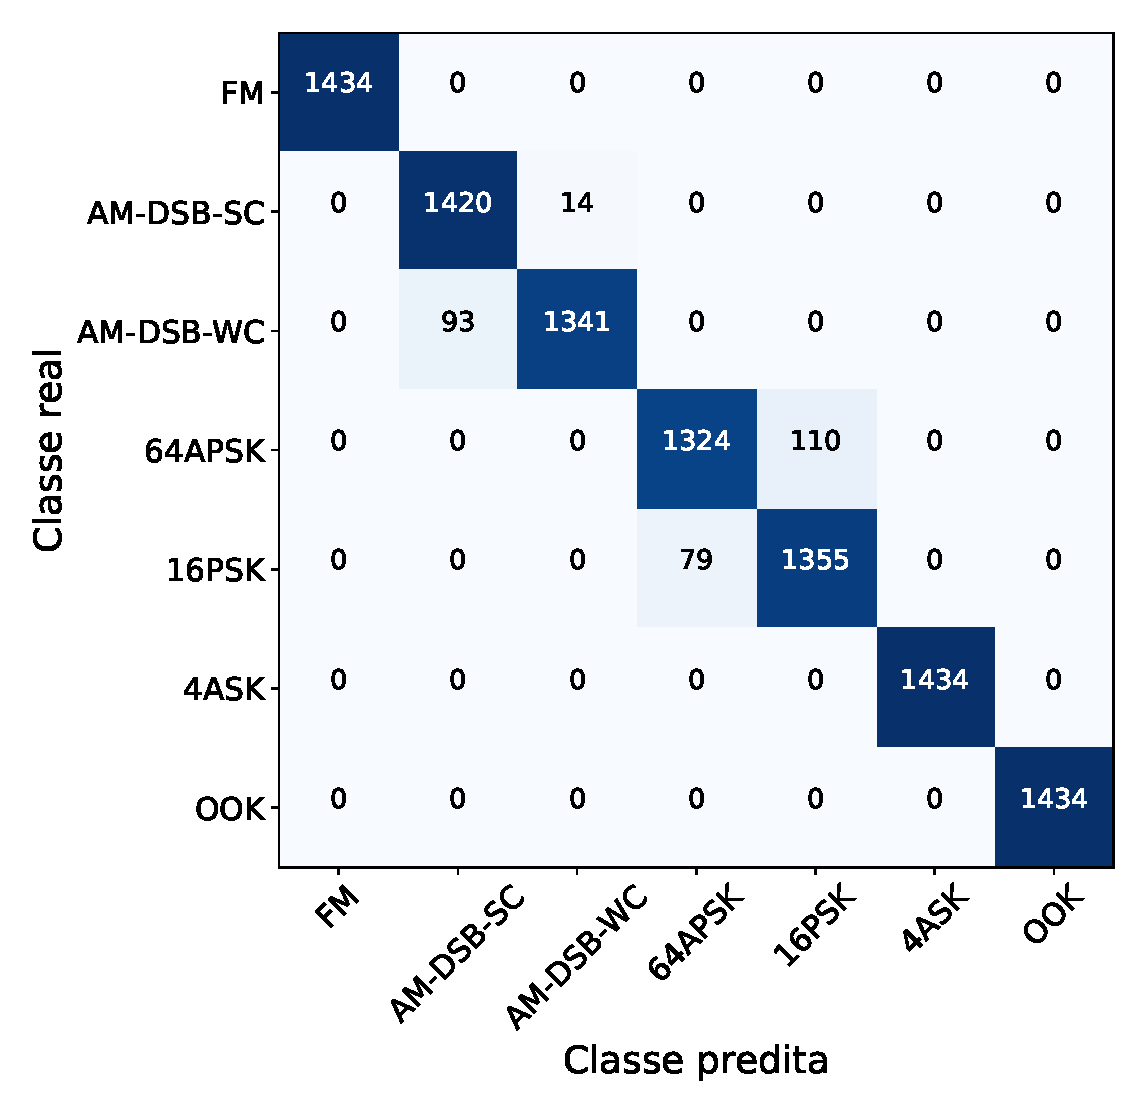
\includegraphics[width=\textwidth]{figuras/cm_nocompress.eps}
    \caption{Modelo não comprimido}
    \label{fig:subfig1}
  \end{subfigure}
  \hfill
  \begin{subfigure}[b]{0.45\textwidth}
    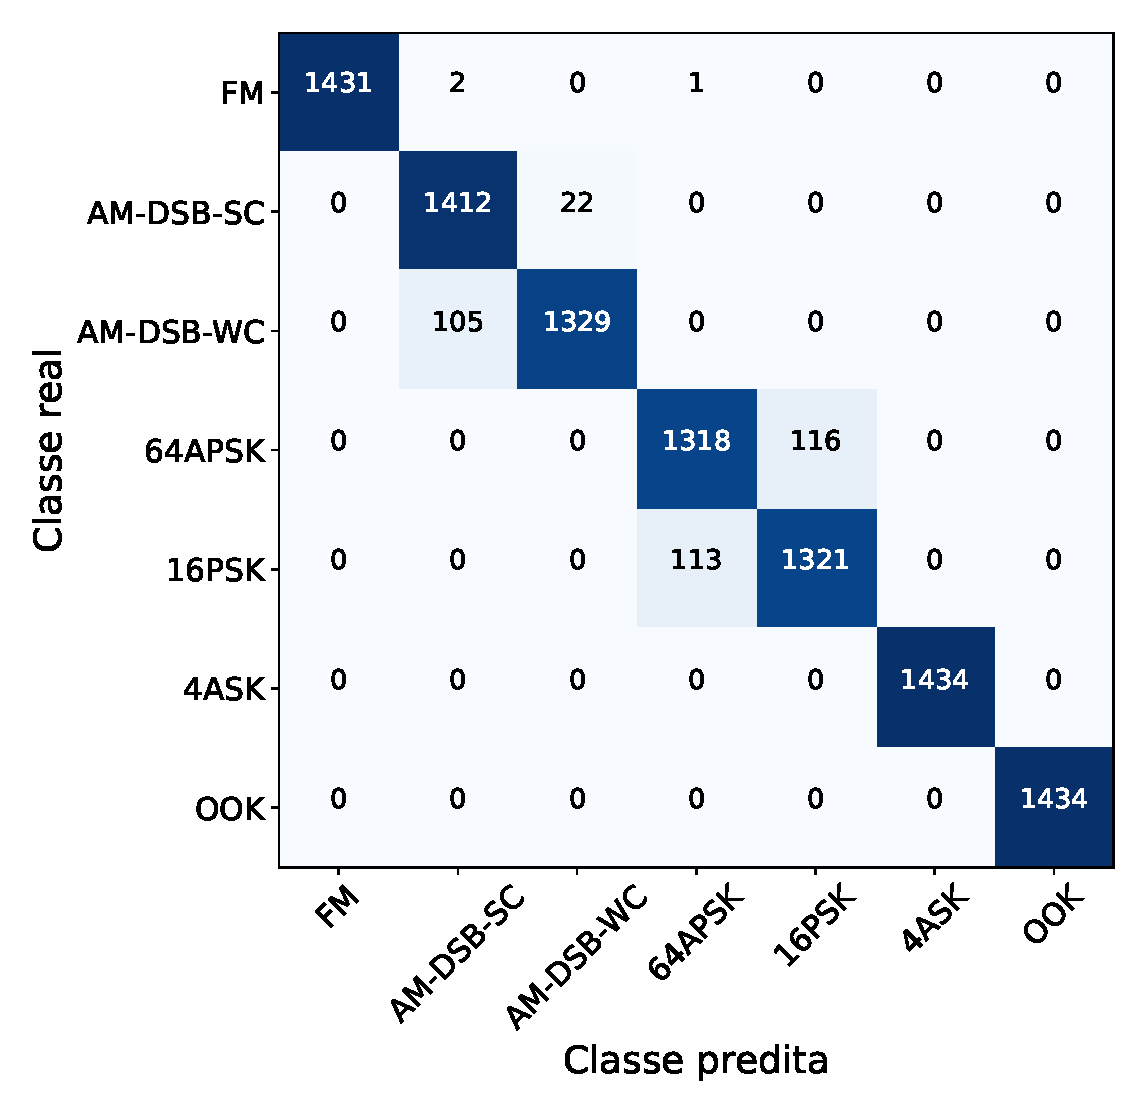
\includegraphics[width=\textwidth]{figuras/cm_8_050.eps}
    \caption{$8$ bits e $\alpha=0,50$}
    \label{fig:subfig2}
  \end{subfigure}
  \caption{Matrizes de confusão de alguns modelos obtidos apos o treinamento}
  \end{figure}

\end{frame}

\begin{frame}{Resultados}
    \begin{figure}[H]
  \centering

  \begin{subfigure}[b]{0.45\textwidth}
    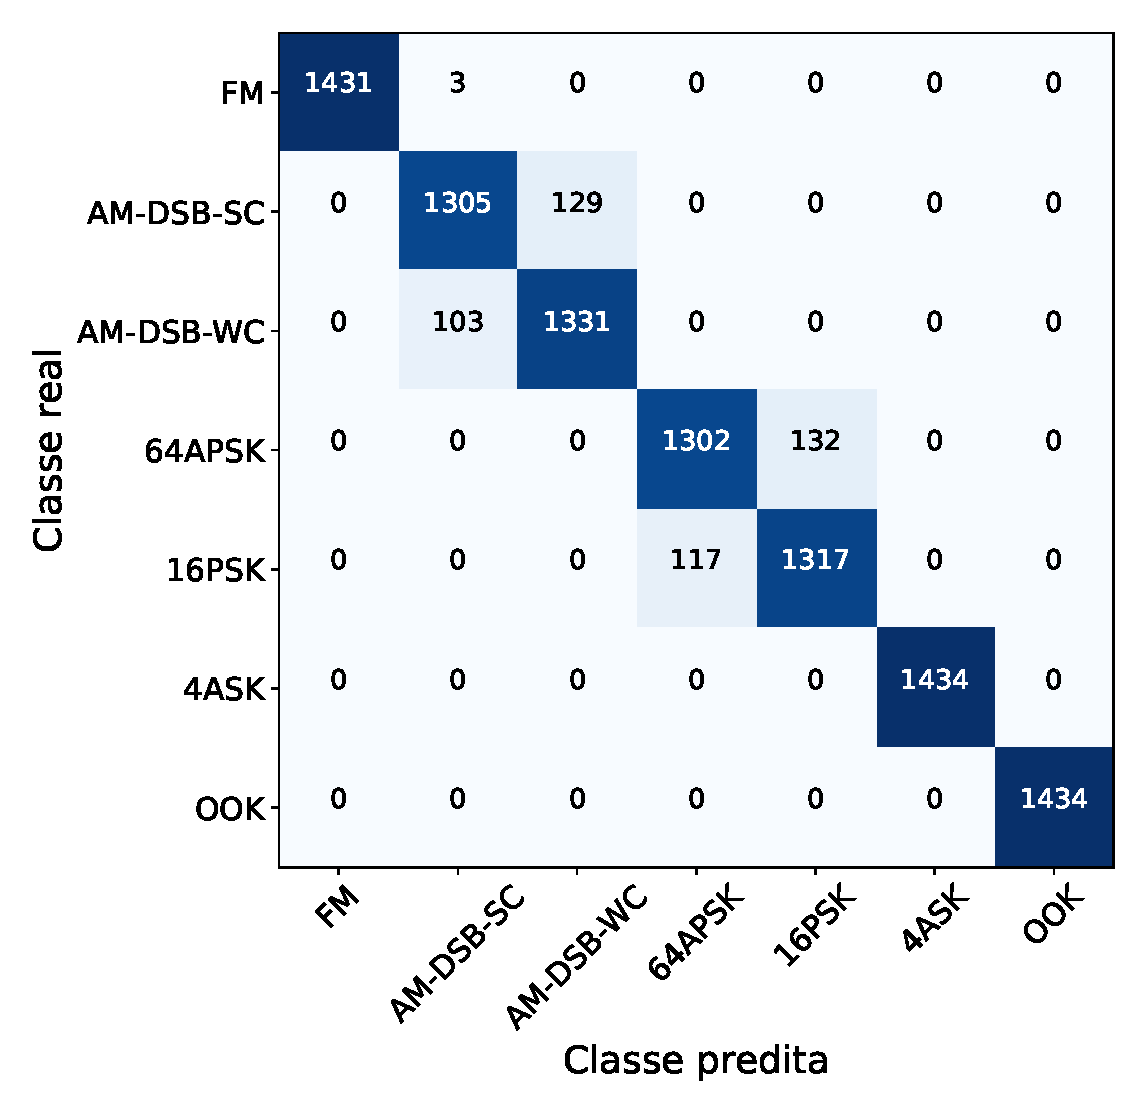
\includegraphics[width=\textwidth]{figuras/cm_8_075.eps}
    \caption{$8$ bits e $\alpha=0,75$}
    \label{fig:subfig1}
  \end{subfigure}
  \hfill
  \begin{subfigure}[b]{0.45\textwidth}
    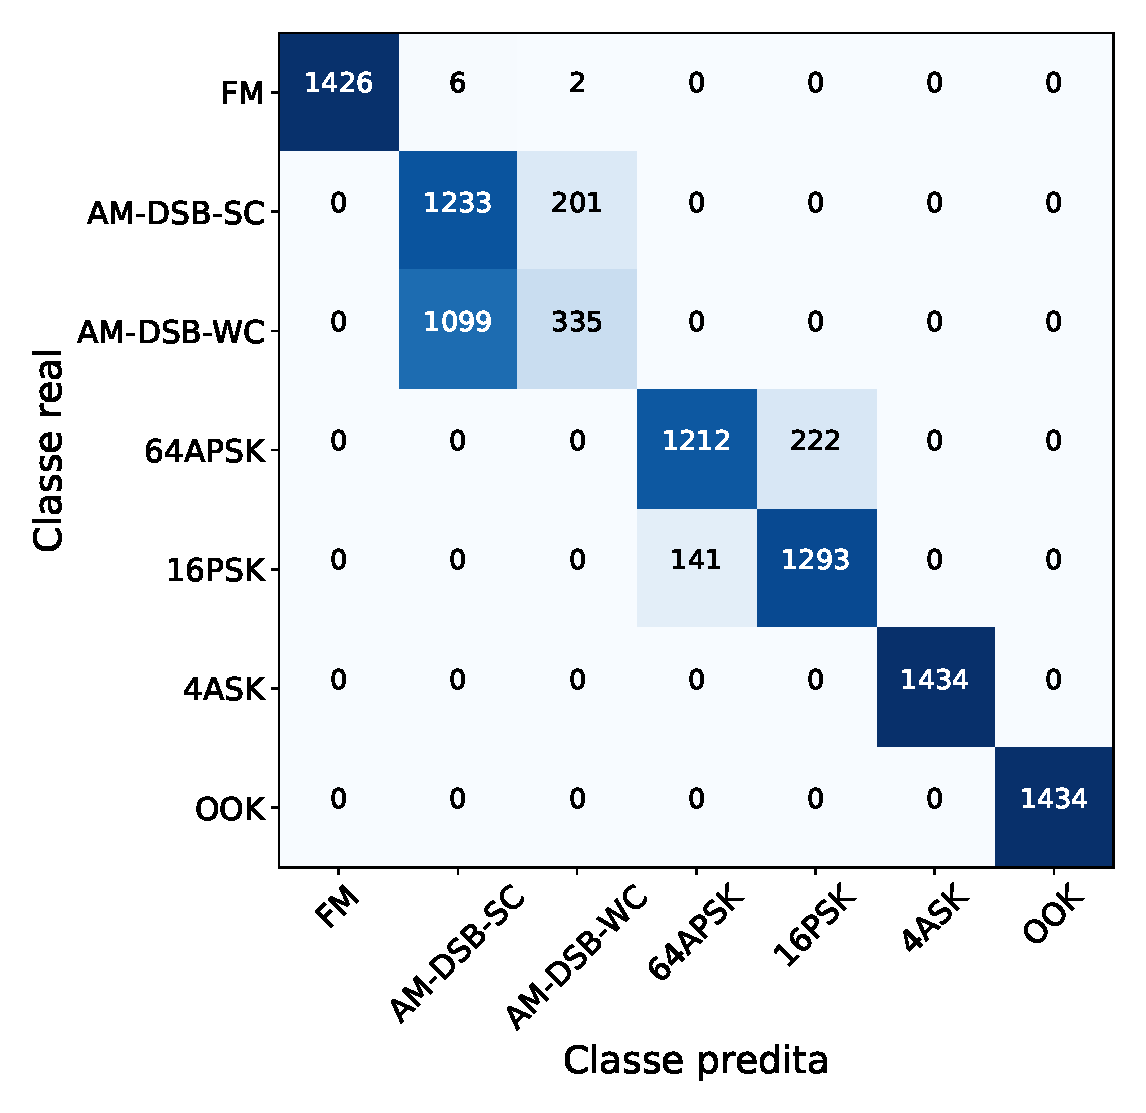
\includegraphics[width=\textwidth]{figuras/cm_3_075.eps}
    \caption{$3$ bits e $\alpha=0,75$}
    \label{fig:subfig2}
  \end{subfigure}
  \caption{Matrizes de confusão de alguns modelos obtidos apos o treinamento}
  \end{figure}

\end{frame}


% Resultados
\section{Compressão para Microserviços}

\begin{frame}{Compressão de modelos para microserviços}
    \begin{itemize}
        \item Microserviços são um estilo arquitetural que tem ganhado crescente popularidade nos últimos anos devido à sua abordagem ágil e escalável para o desenvolvimento de aplicações;
        \item Em ambientes de microserviços, o uso de recursos é uma preocupação importante;
        \item Modelos de DNNs, especialmente os mais complexos, podem requisitar um grande consumo de memória, processamento e tempo de inferência. O que pode ser problemático para esses ambientes.
        \item O uso de estratégias de compressão de modelos de DNN pode afetar positivamente o desempenho e uso eficiente dos recursos computacionais de microserviços;
    \end{itemize}
\end{frame}


\begin{frame}{Compressão de modelos para microserviços}
    \begin{itemize}
        \item A compressão de modelos também pode tornar a implementação e a escalabilidade dos microserviços mais ágeis;
        \item Modelos menores são mais rápidos de transferir e carregar em diferentes ambientes, tornando o processo de implantação mais eficiente.
    \end{itemize}
\end{frame}

\begin{frame}{Dataset}
    \begin{figure}[H]
    \centering
    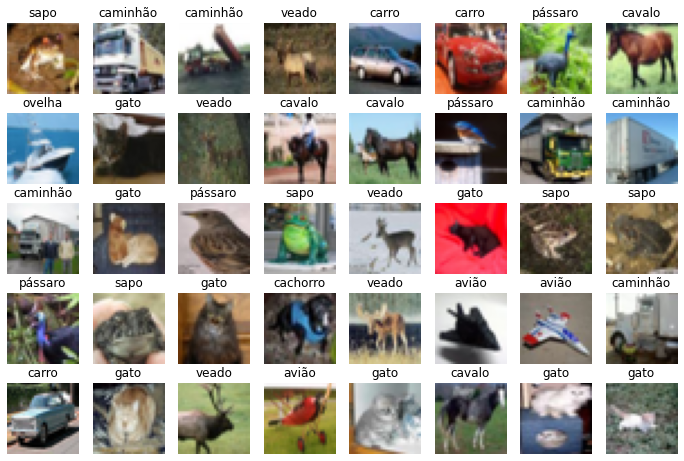
\includegraphics[width=0.65\textwidth]{figuras/cifar10ex.png}
    \caption{Amostra do dataset cifar10}
    \end{figure}
\end{frame}

\begin{frame}{Treinamento da DNN}
    Para o treinamento do modelo, foram escolhidos os seguintes parâmetros:
    \begin{itemize}
        \item Tamanho de cada lote de 64;
        \item Otimizador de Descida de Gradiente Estocástico (SGD);
        \item 60 mil amostras para treino e 10 mil para validação;
        \item Taxa de aprendizagem de 0,05 e momento do 0,9;
        \item Critétio de loss como entropia cruzada de categoria.
    \end{itemize}
\end{frame}

\begin{frame}{Arquitetura do modelo}
O modelo foi definido com a arquitetura VGG16 com duas camadas densas:
\begin{columns}[T,c]
    \column{.5\textwidth}
      \scriptsize
      \begin{itemize}
        \item Entrada($32 \times 3 \times 3$);
        \item Conv2D($64 \times 3 \times 3$) e ReLU;
        \item Conv2D($64 \times 3 \times 3$) e ReLU;
        \item MaxPool($2 \times 2$);
        \item Conv2D($128 \times 3 \times 3$) e ReLU;
        \item Conv2D($128 \times 3 \times 3$) e ReLU;
        \item MaxPool($2 \times 2$);
        \item Conv2D($256 \times 3 \times 3$) e ReLU;
        \item Conv2D($256 \times 3 \times 3$) e ReLU;
        \item Conv2D($256 \times 3 \times 3$) e ReLU;
        \item MaxPool($2 \times 2$);
      \end{itemize}
    \column{.5\textwidth}
      \scriptsize
      \begin{itemize}
        \item Conv2D($512 \times 3 \times 3$) e ReLU;
        \item Conv2D($512 \times 3 \times 3$) e ReLU;
        \item Conv2D($512 \times 3 \times 3$) e ReLU;
        \item MaxPool($2 \times 2$);
        \item Conv2D($512 \times 3 \times 3$) e ReLU;
        \item Conv2D($512 \times 3 \times 3$) e ReLU;
        \item Conv2D($512 \times 3 \times 3$) e ReLU;
        \item MaxPool($2 \times 2$);
        \item Dense($4096$) e ReLU;
        \item Dense($4096$) e ReLU;
        \item Dense($10$) e Softmax.
      \end{itemize}
    \end{columns}
\end{frame}

\begin{frame}{Resultados do treinamento}
    \scriptsize
    \begin{table}[H]
        \caption{\scriptsize{Acurácias obtidas na classificação de imagens a partir do modelo comprimido para vários valores de quantidade de bits e $\alpha$.}}
        \centering
        \begin{tabular}{l|llll}
        \hline
        \textbf{\diagbox{bits}{$\alpha$}} & \textbf{0,00}  & \textbf{0,50} & \textbf{1,50} & \textbf{1,25}\\ \hline
        \textbf{32 bits} &	81,58\%	& 79,39\% & 79,53\% & 74,64\%\\
        \textbf{8 bits} & 79,76\%	& 80,77\% & 79,31\% & 74,42\%\\\hline
        \end{tabular}
        \end{table}
    \scriptsize
    \begin{table}[H]
        \caption{\scriptsize{Esparsidades obtidas na classificação de imagens a partir do modelo comprimido para vários valores de tamanho de bits e $\alpha$.}}
        \centering
        \begin{tabular}{l|lll}
        \hline
        \textbf{\diagbox{bits}{$\alpha$}}  & \textbf{0,50} & \textbf{1,50} & \textbf{1,25}\\ \hline
        \textbf{32 bits} & 37,92\% & 62,76\% & 74,76\%\\
        \textbf{8 bits} & 36,94\% & 60,68\% & 74,49\%\\\hline
        \end{tabular}
        \end{table}
\end{frame}

\begin{frame}{Resultados do treinamento}
    \begin{figure}[H]
  \centering

  \begin{subfigure}[b]{0.49\textwidth}
    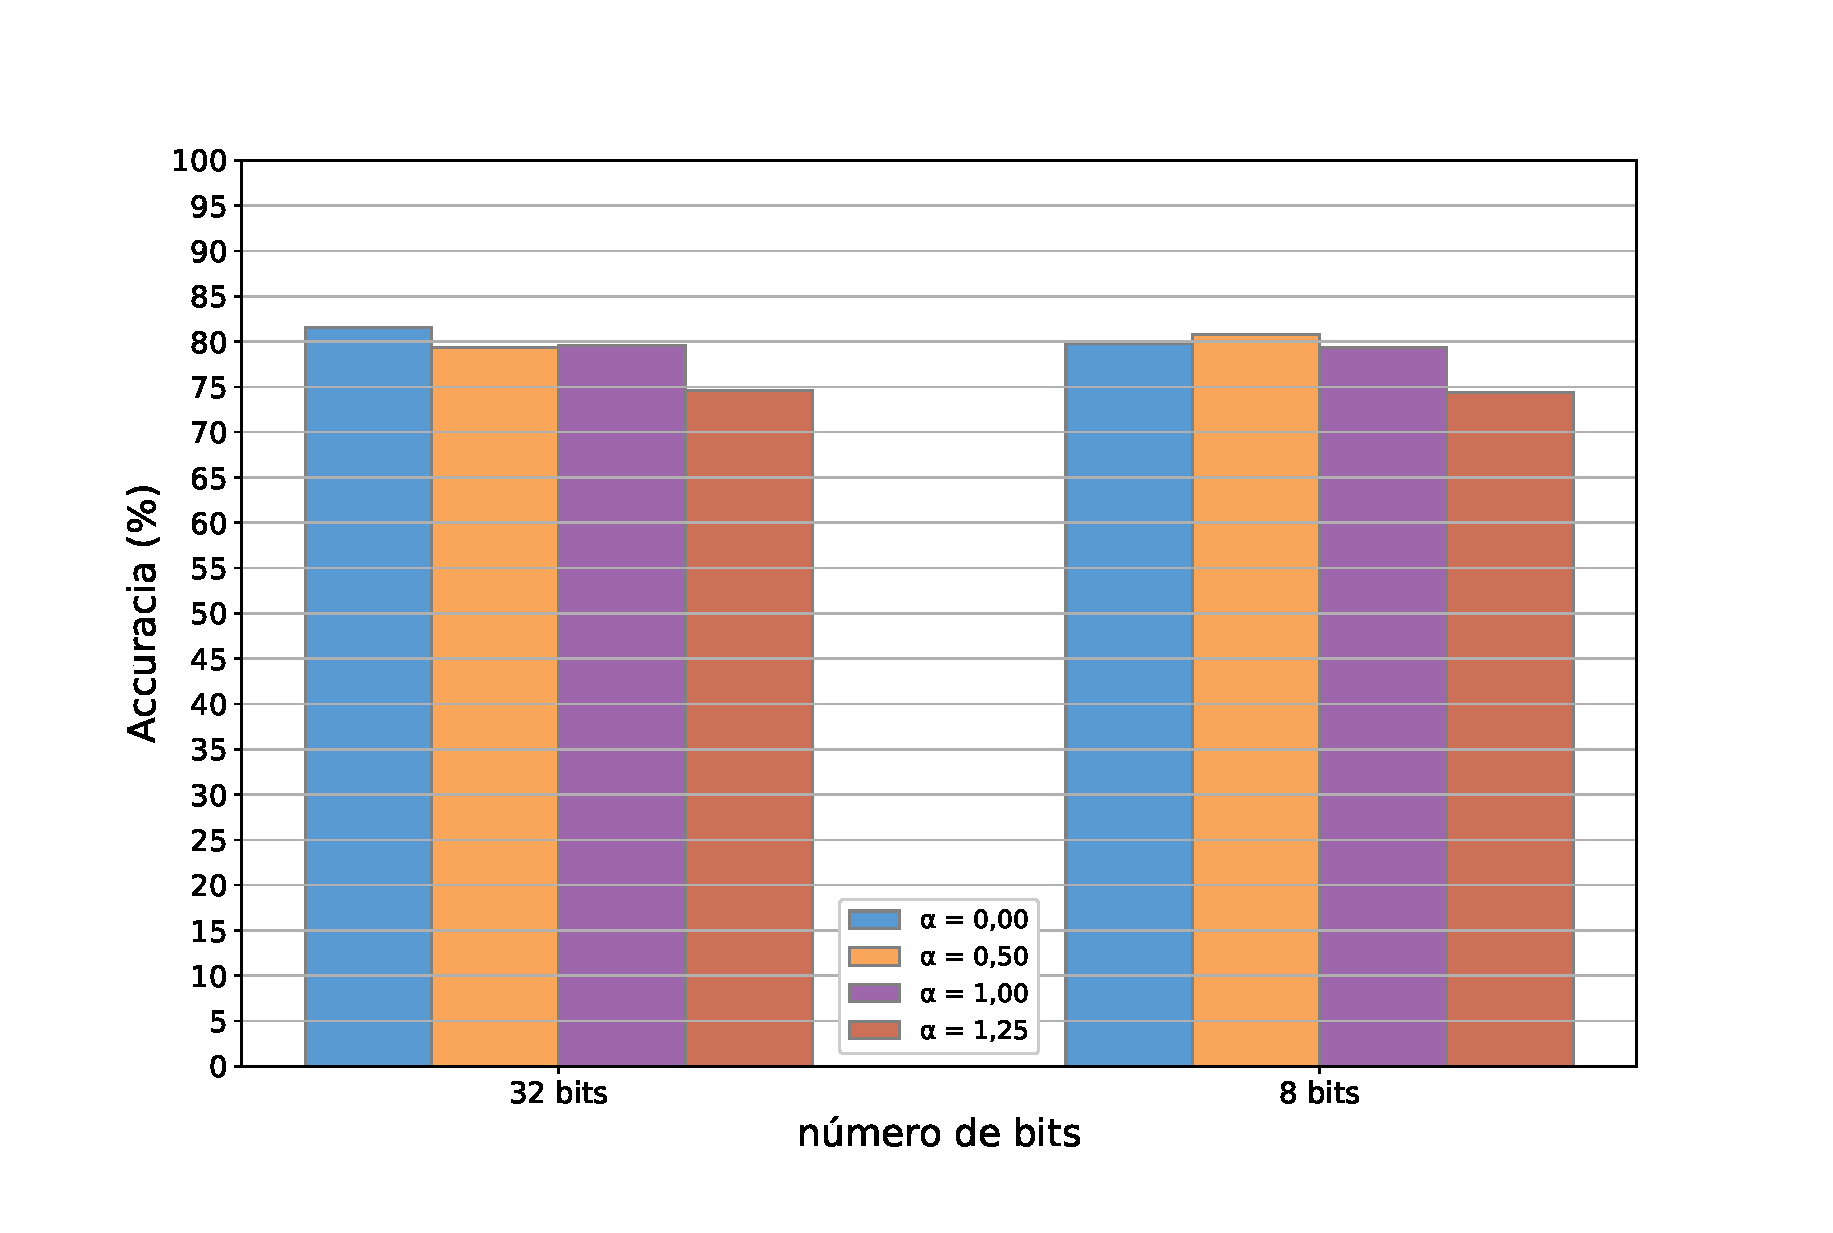
\includegraphics[width=\textwidth]{figuras/cifar_acc_fig.eps}
    \caption{Acurácia dos modelos}
  \end{subfigure}
  \hfill
  \begin{subfigure}[b]{0.49\textwidth}
    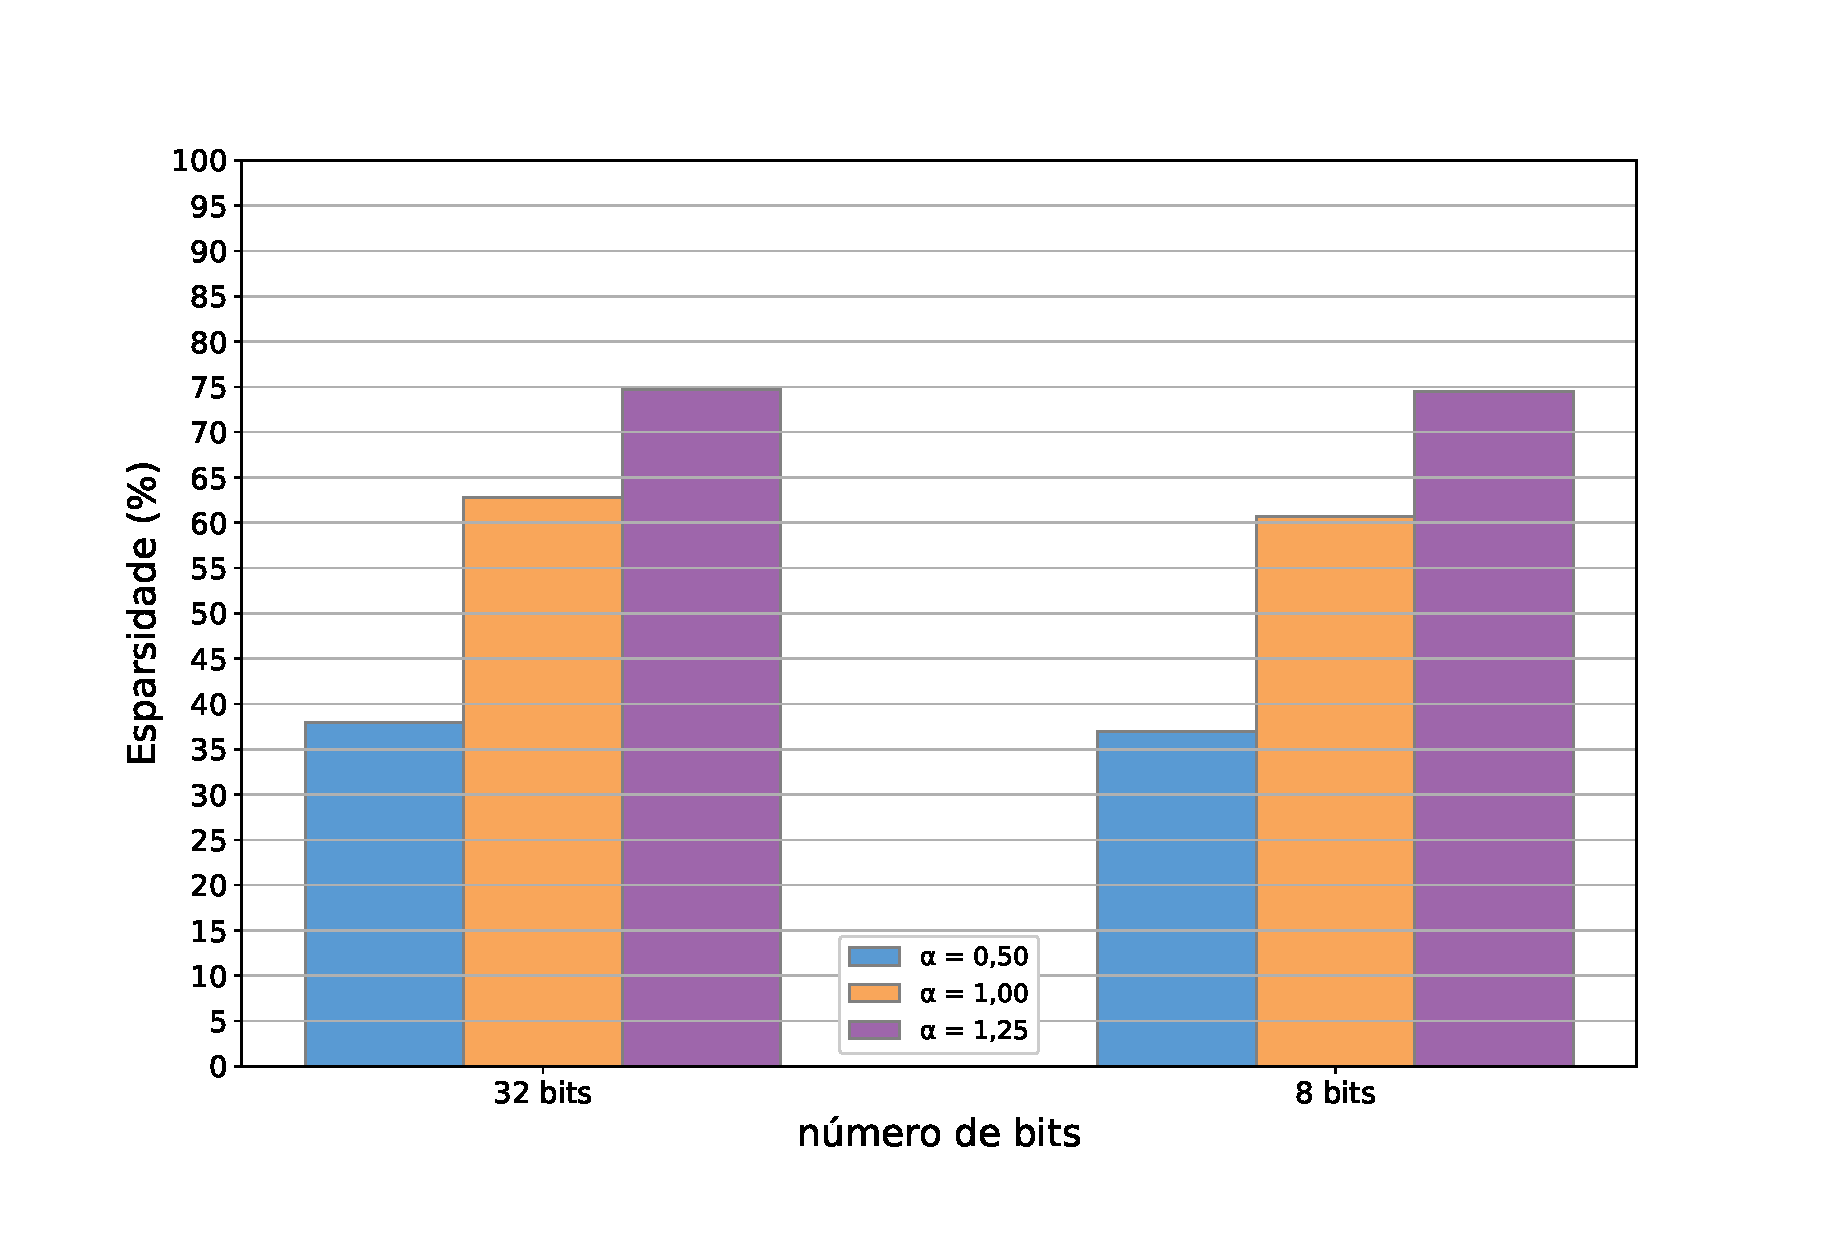
\includegraphics[width=\textwidth]{figuras/cifar_sparsity_fig.eps}
    \caption{Esparsidade dos modelos}
  \end{subfigure}
  \caption{Acurácias e esparsidades obtidas na classificação de imagens a partir do modelo comprimido para vários valores de tamanho de bits e $\alpha$.}
  \end{figure}
\end{frame}

\begin{frame}{Resultados do treinamento}
    \begin{figure}[H]
        \centering
        \begin{subfigure}[b]{0.49\textwidth}
          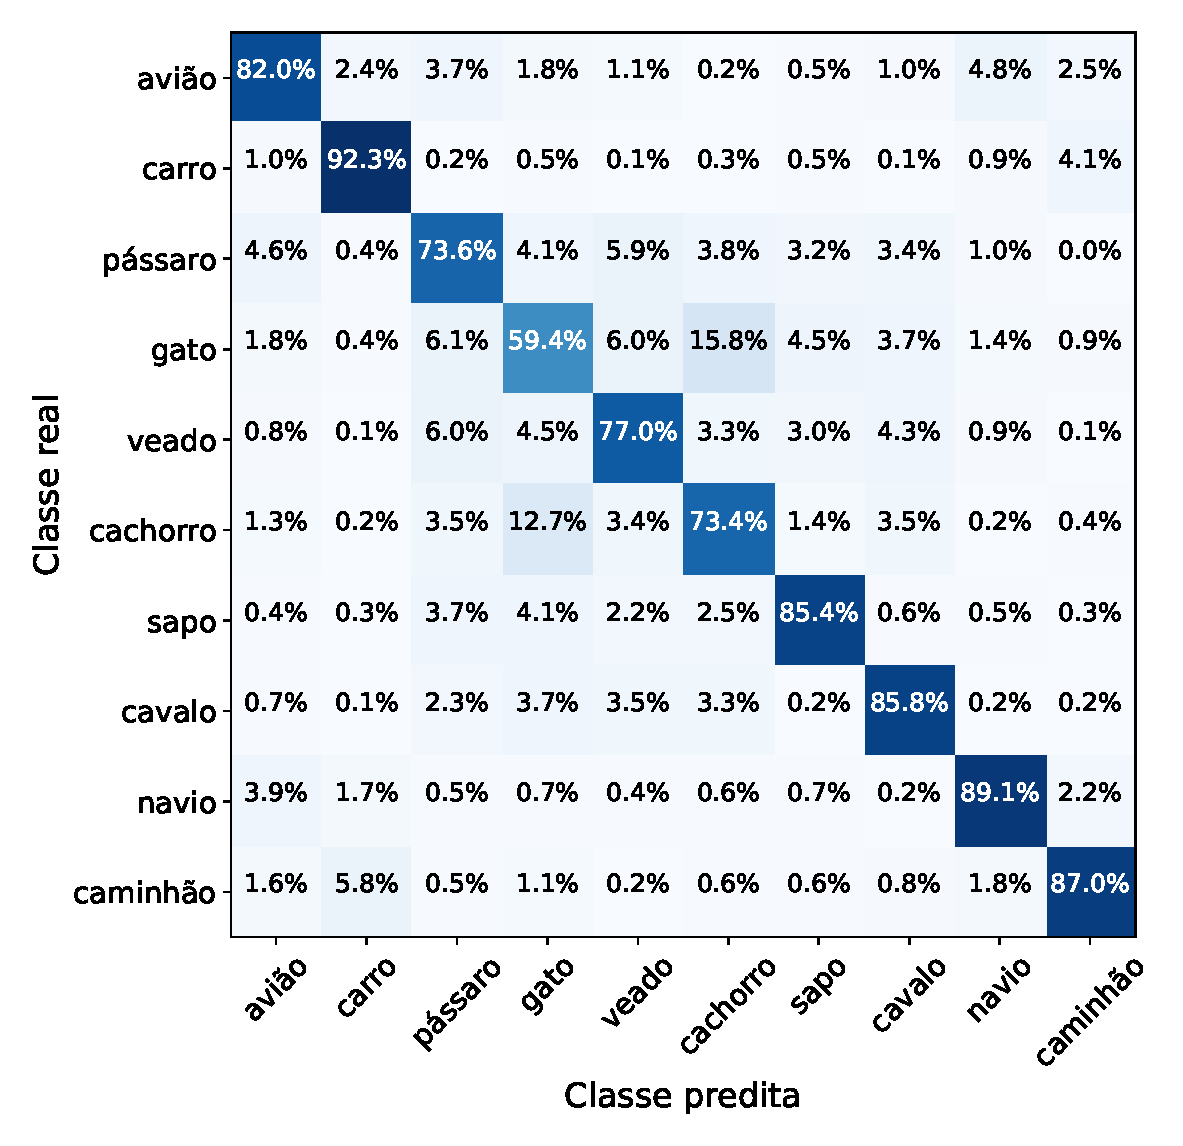
\includegraphics[width=\textwidth]{figuras/cifar_no_compress.eps}
          \caption{Modelo não comprimido}
        \end{subfigure}
        \hfill
        \begin{subfigure}[b]{0.49\textwidth}
          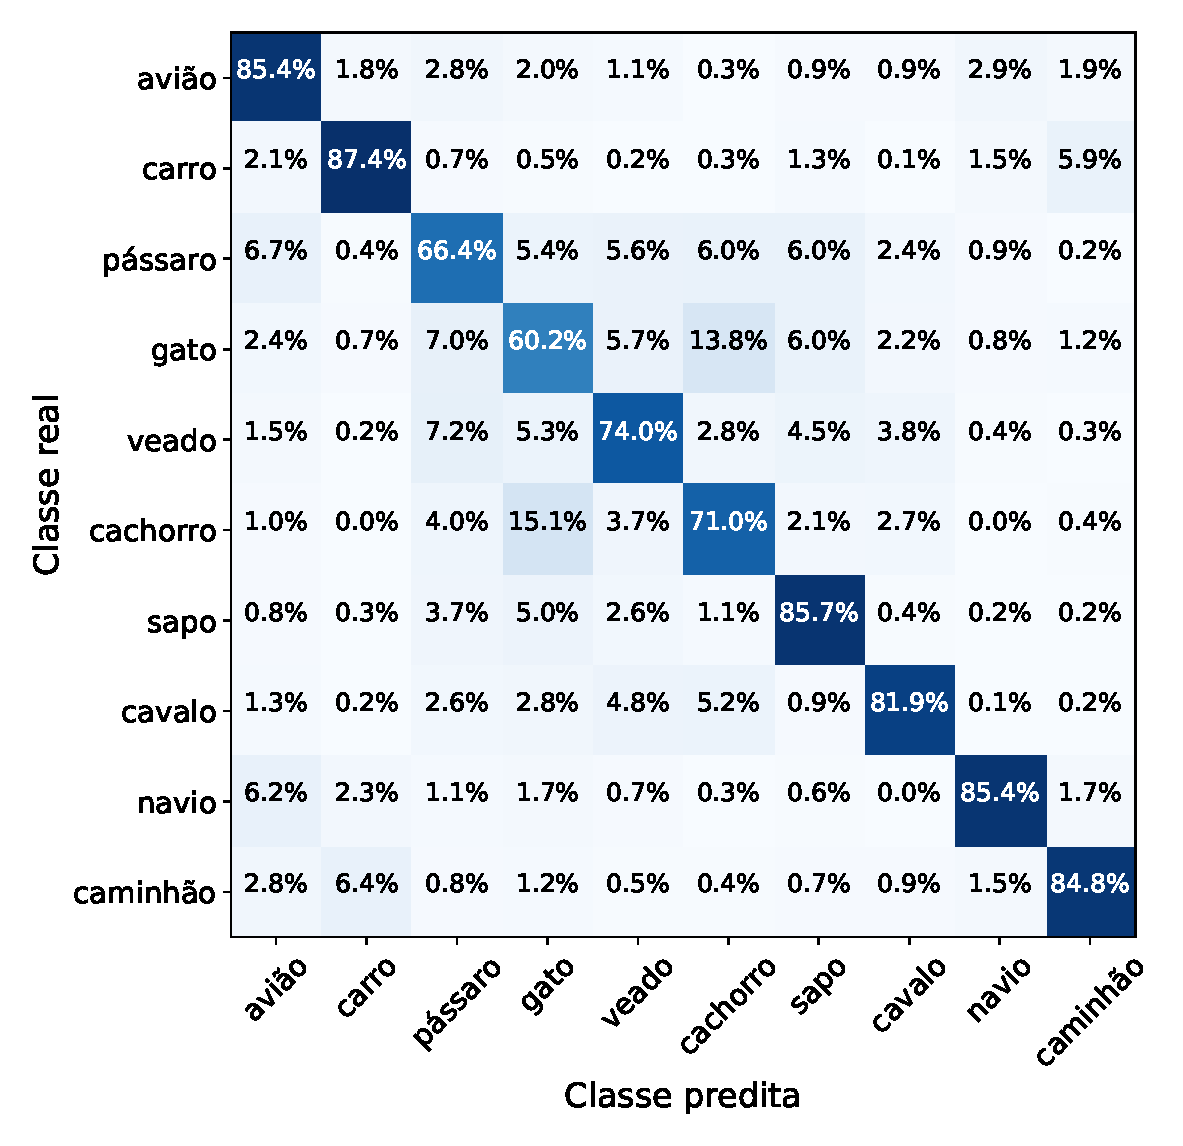
\includegraphics[width=\textwidth]{figuras/cifar_q8_p75.eps}
          \caption{8 bits e $\alpha = 1,25$}
        \end{subfigure}
        \caption{Matrizes de confusão do modelo sem compressão e do mais comprimido.}
    \end{figure}
\end{frame}


\begin{frame}{Resultados do treinamento}
    \begin{table}[H]
        \caption{Tamanho do modelo comprimido para vários valores de quantidade de bits e $\alpha$ em MegaBytes após compressão por Deflate}
        \centering
        \begin{tabular}{l|llll}
        \hline
        \textbf{\diagbox{bits}{$\alpha$}} & \textbf{0,00}  & \textbf{0,50} & \textbf{1,50} & \textbf{1,25}\\ \hline
        \textbf{32 bits} & 123,51MB	& 87,11MB & 55,80MB & 39,39MB\\
        \textbf{8 bits} & 32,50MB & 32,12MB & 22,09MB & 16,20MB\\\hline
        \end{tabular}
        \end{table}
\end{frame}

\begin{frame}{Resultados do treinamento}
    \begin{figure}[H]
        \centering
        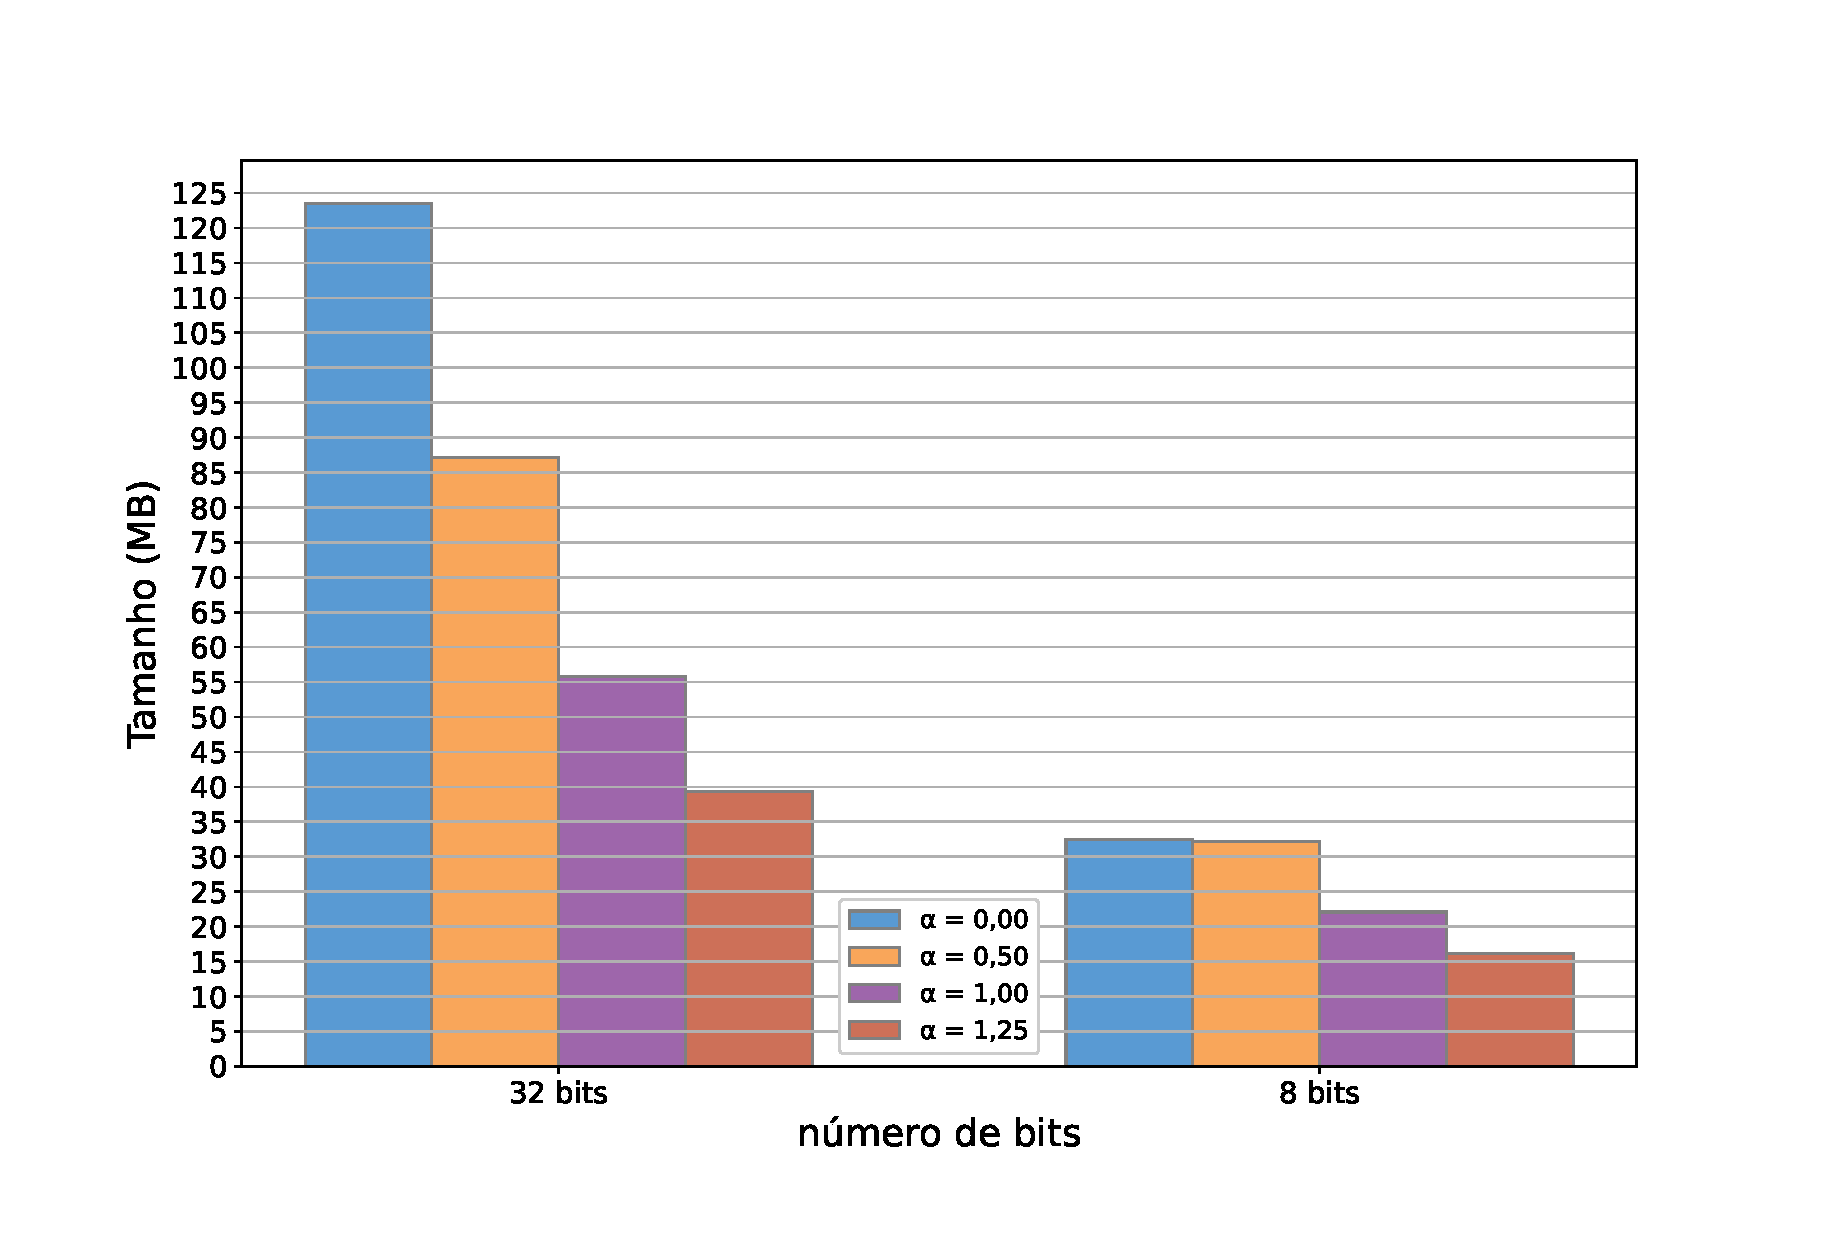
\includegraphics[width=0.7\textwidth]{figuras/cifar_mb_size_fig.eps}
        \caption{Tamanho do modelo comprimido para vários valores de quantidade de bits e $\alpha$ em MegaBytes após compressão por Deflate}
        \end{figure}
\end{frame}

\begin{frame}{Infraestrutura}
    \begin{figure}[H]
    \centering
    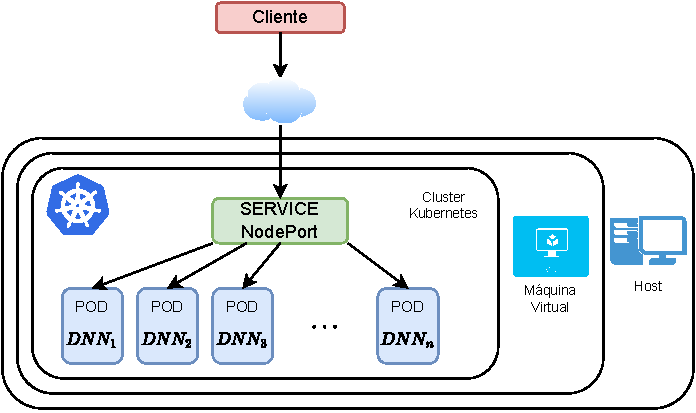
\includegraphics[width=0.7\textwidth]{figuras/infra.pdf}
    \caption{Infraestrutura geral desenvolvida}
    \end{figure}
\end{frame}

\begin{frame}{Configurações dos pods}
    Cada pod foi construído com as seguintes características:
    \begin{itemize}
        \item Máximo de memória em 100MiB;
        \item Máximo de processamento em 100miliCPU;
        \item Nova réplica com 20\% do máximo de processamento;
        \item Máximo de 10 réplicas.
    \end{itemize}
\end{frame}

\begin{frame}{Perfil de estresse}
    Foram criados perfis de estresse utilizando o \textit{Open Model Thread Group} da ferramenta Apache JMeter, para variar a quantidade de requisições do sistema com o passar do tempo.
    \begin{figure}[H]
    \centering
    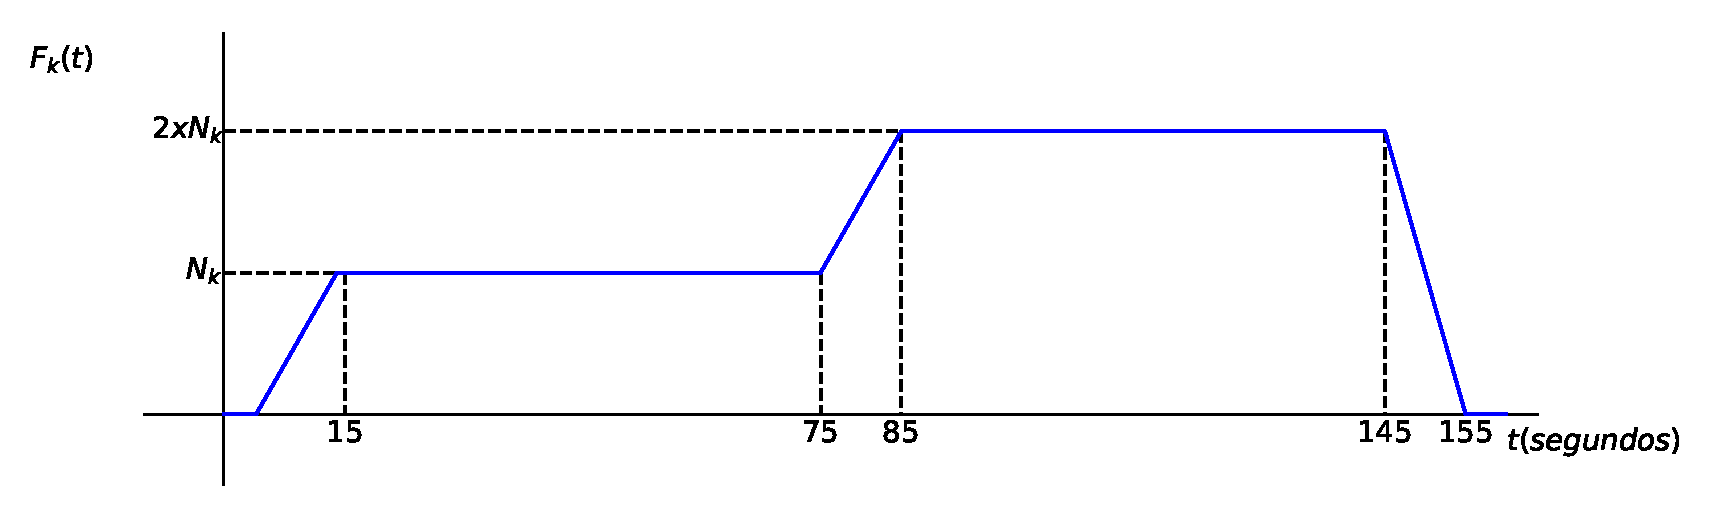
\includegraphics[width=1\textwidth]{figuras/estresse.eps}
    \caption{Perfil de estresse com $n$ variando em $75$, $125$ e $250$}
    \end{figure}
\end{frame}

\begin{frame}{Resultados}
    \scriptsize
    \begin{table}[H]
        \caption{\scriptsize{Latência de resposta das requisições, Consumo de memória e processamento de cada microseriviço do primeiro perfil de estresse $N_1 = 75$.}}
        \centering
        \begin{tabular}{llllll} \\
        \hline
        \textbf{bits} & \textbf{$\alpha$}  &  \textbf{Latência} & \textbf{Memória} &\textbf{CPU}\\  \hline
        32 &0,00& $16,23ms \pm 2,988$ & 701MiB & 135miliCPU\\
        32 &0,50& $15,97ms \pm 3,467$ & 707MiB & 136miliCPU\\
        32 &1,00& $16,02ms \pm 2,659$ & 701MiB & 143miliCPU\\
        32 &1,25& $15,44ms \pm 2,597$ & 703MiB & 132miliCPU\\
        8  &0,00& $9,39ms \pm 2,026$ & 412MiB & 95miliCPU\\
        8  &0,50& $9,27ms \pm 3,011$ & 414MiB & 94miliCPU\\
        8  &1,00& $9,57ms \pm 2,144$ & 411MiB & 96miliCPU\\
        8  &1,25& $9,44ms \pm 1,729$ & 411MiB & 94miliCPU\\
        \hline
        \end{tabular}
        \end{table}
\end{frame}

\begin{frame}{Resultados}
    \begin{figure}[H]
        \centering
        \begin{subfigure}[b]{0.32\textwidth}
            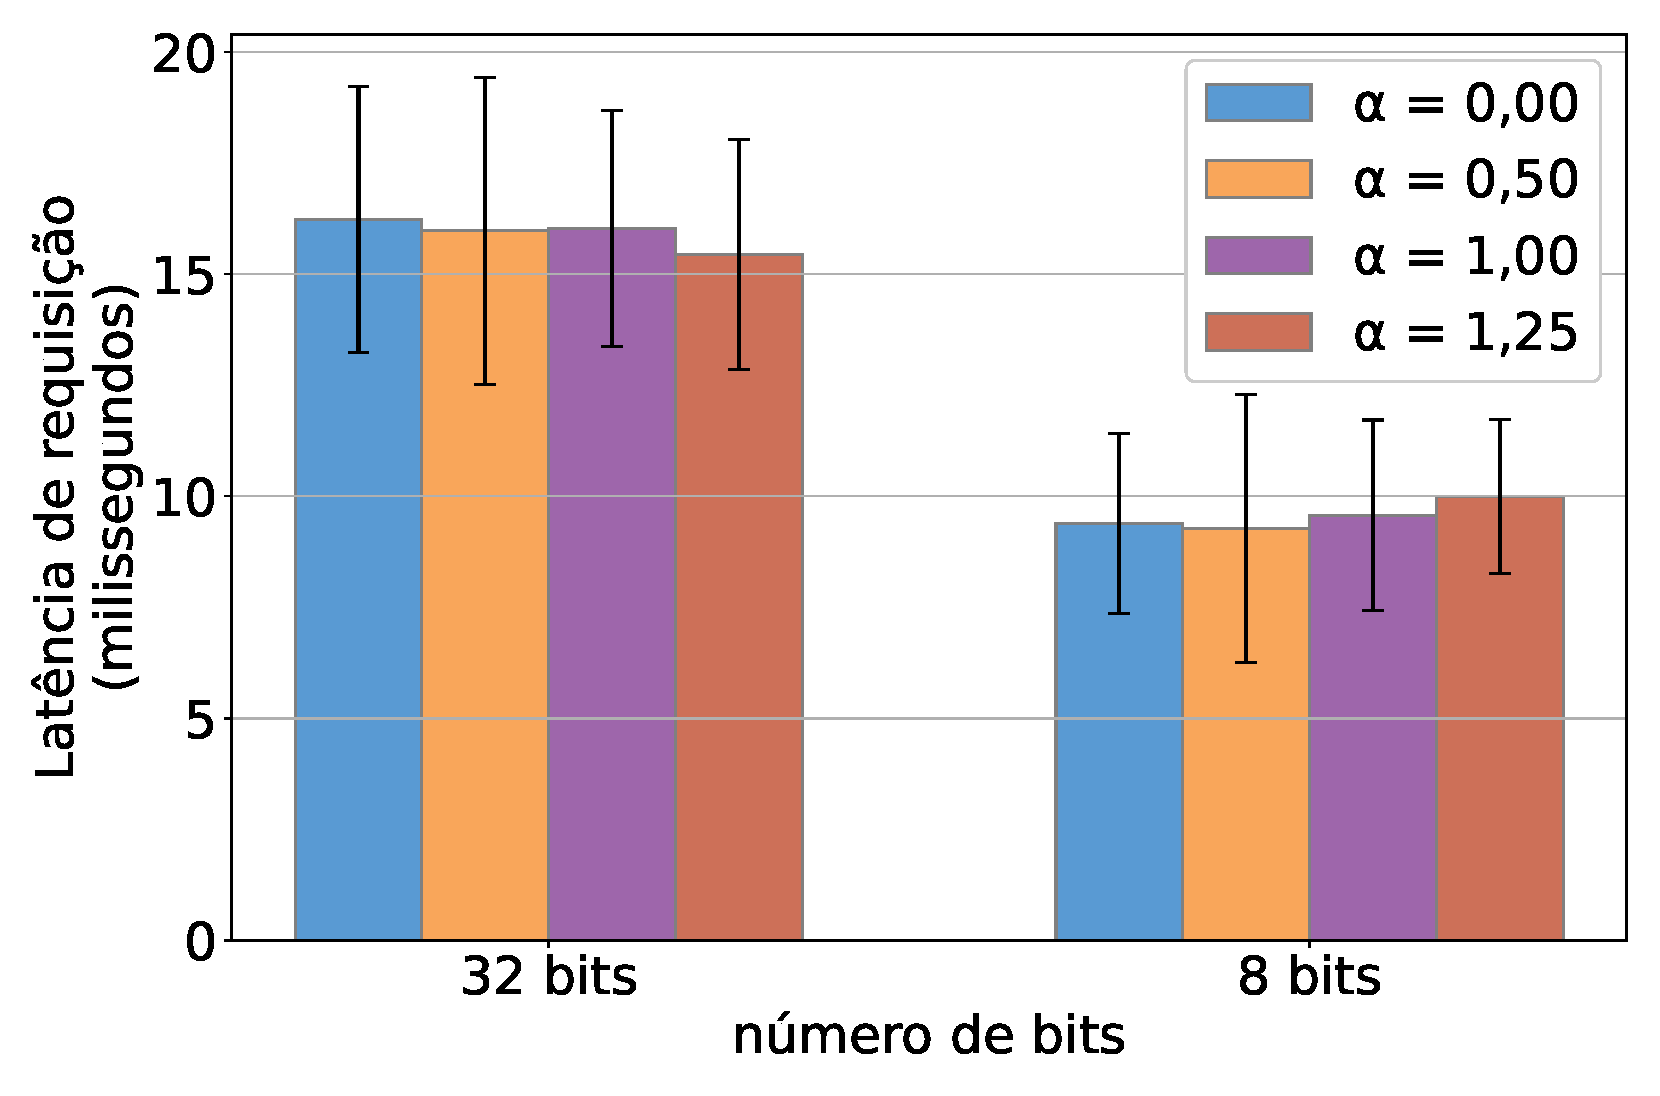
\includegraphics[width=\textwidth]{figuras/latencia1.eps}
            \caption{\scriptsize{Latências}}
          \end{subfigure}  
          \begin{subfigure}[b]{0.32\textwidth}
            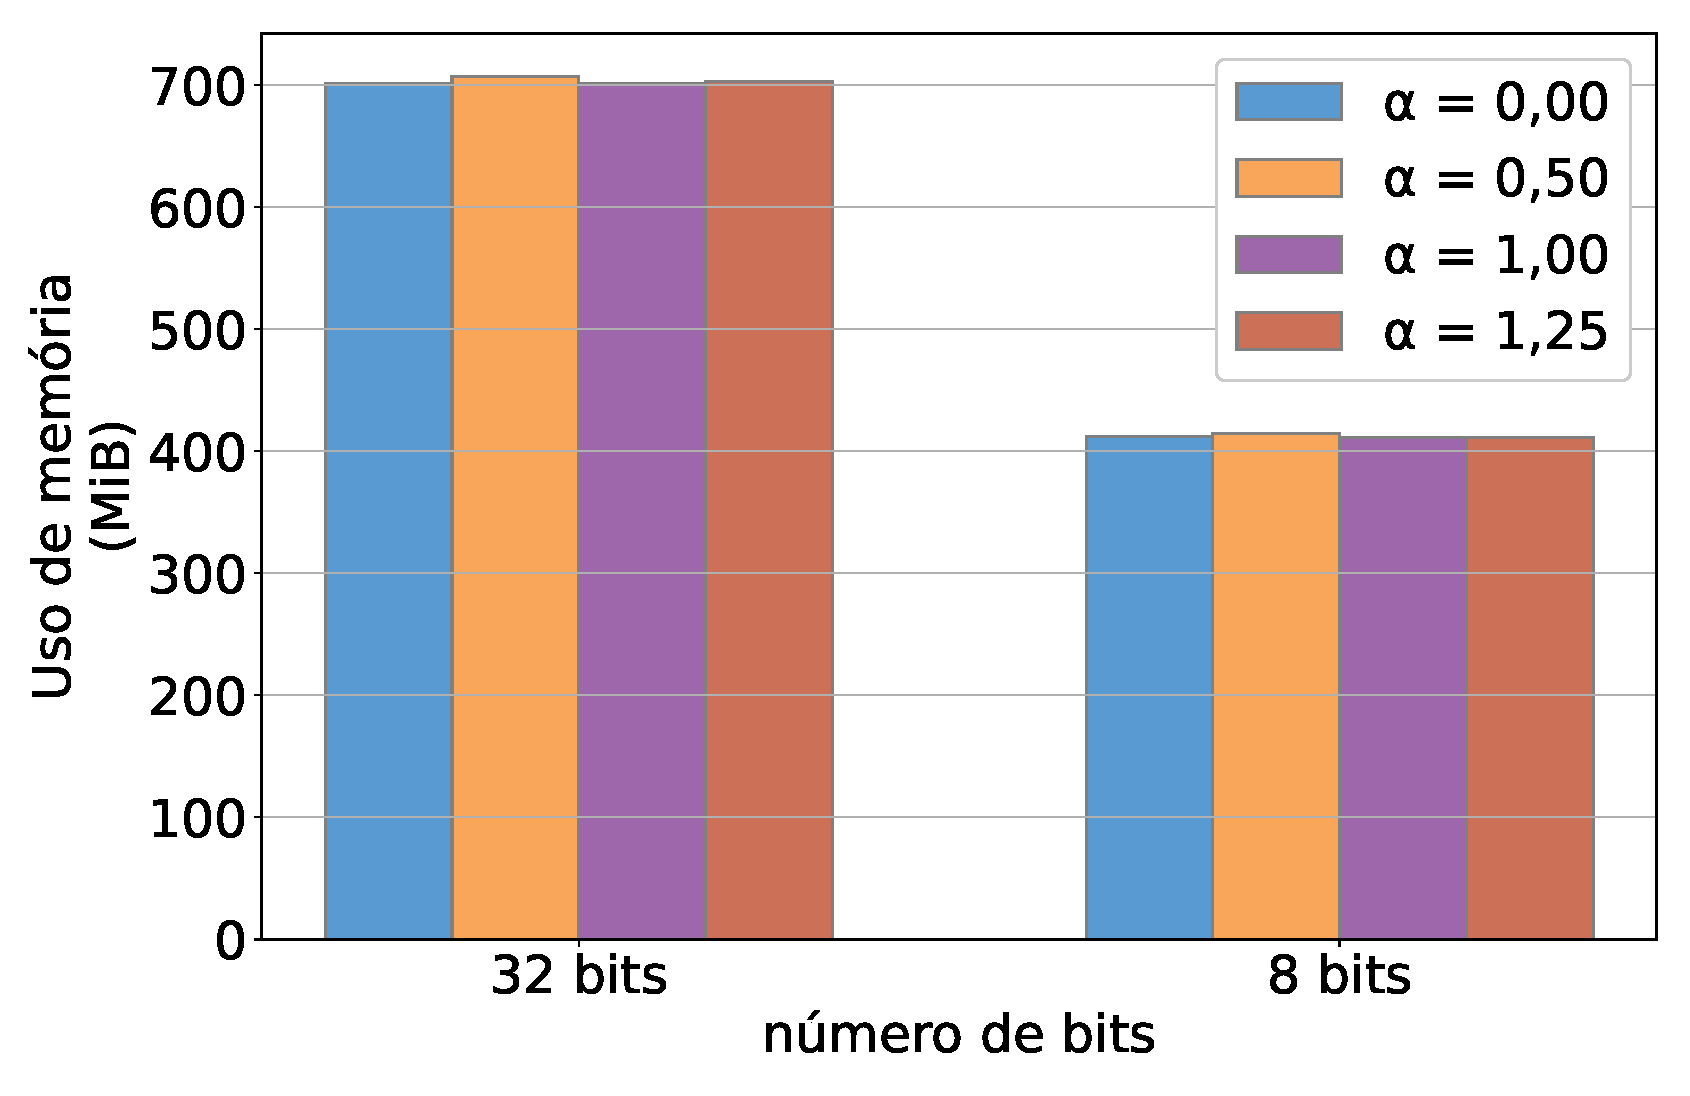
\includegraphics[width=\textwidth]{figuras/memoria1.eps}
            \caption{\scriptsize{Consumo de memória}}
        \end{subfigure}
        \begin{subfigure}[b]{0.32\textwidth}
            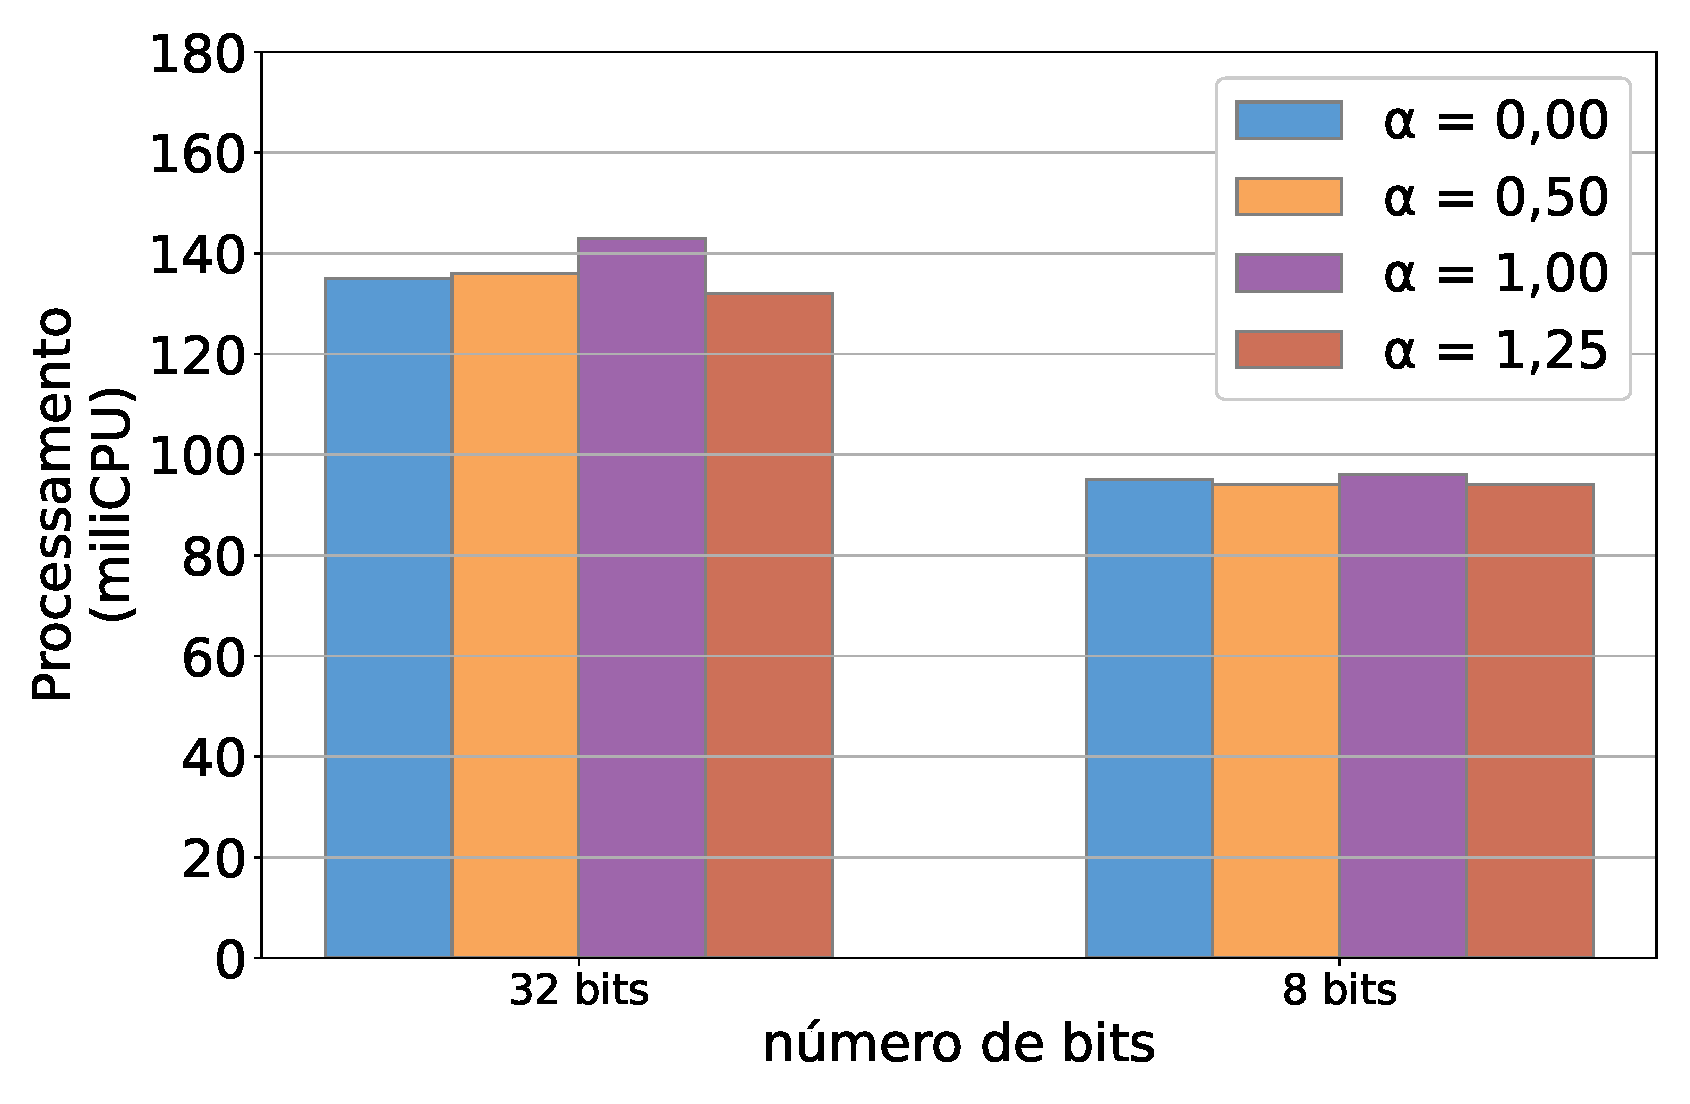
\includegraphics[width=\textwidth]{figuras/cpu1.eps}
            \caption{\scriptsize{Processamento}}
        \end{subfigure}
        \caption{\scriptsize{Latência de resposta em milissegundos, consumo de memória e uso de CPU de cada microserviço para o primeiro perfil de estresse $N_1 = 75$.}}
        \end{figure}
\end{frame}


\begin{frame}{Resultados}
    \scriptsize
    \begin{table}[H]
        \caption{\scriptsize{Latência de resposta das requisições, Consumo de memória e processamento de cada microseriviço do segundo perfil de estresse $N_2 = 125$.}}
        \centering
        \begin{tabular}{llllll} \\
        \hline
        \textbf{bits} & \textbf{$\alpha$}  &  \textbf{Latência} & \textbf{Memória} &\textbf{CPU}\\  \hline
        32 &0,00& $16,01ms \pm 2,755$ & 701MiB & 136miliCPU\\
        32 &0,50& $16,44ms \pm 3,134$ & 704MiB & 137miliCPU\\
        32 &1,00& $15,51ms \pm 2,299$ & 703MiB & 139miliCPU\\
        32 &1,25& $15,23ms \pm 3,101$ & 703MiB & 136miliCPU\\
        8  &0,00& $9,22ms \pm 2,577$ & 411MiB & 94miliCPU\\
        8  &0,50& $8,68ms \pm 3,822$ & 412MiB & 94miliCPU\\
        8  &1,00& $8,67ms \pm 3,715$ & 411MiB & 95miliCPU\\
        8  &1,25& $9,58ms \pm 3,122$ & 411MiB & 94miliCPU\\
        \hline
        \end{tabular}
        \end{table}
\end{frame}

\begin{frame}{Resultados}
    \begin{figure}[H]
        \centering
        \begin{subfigure}[b]{0.32\textwidth}
            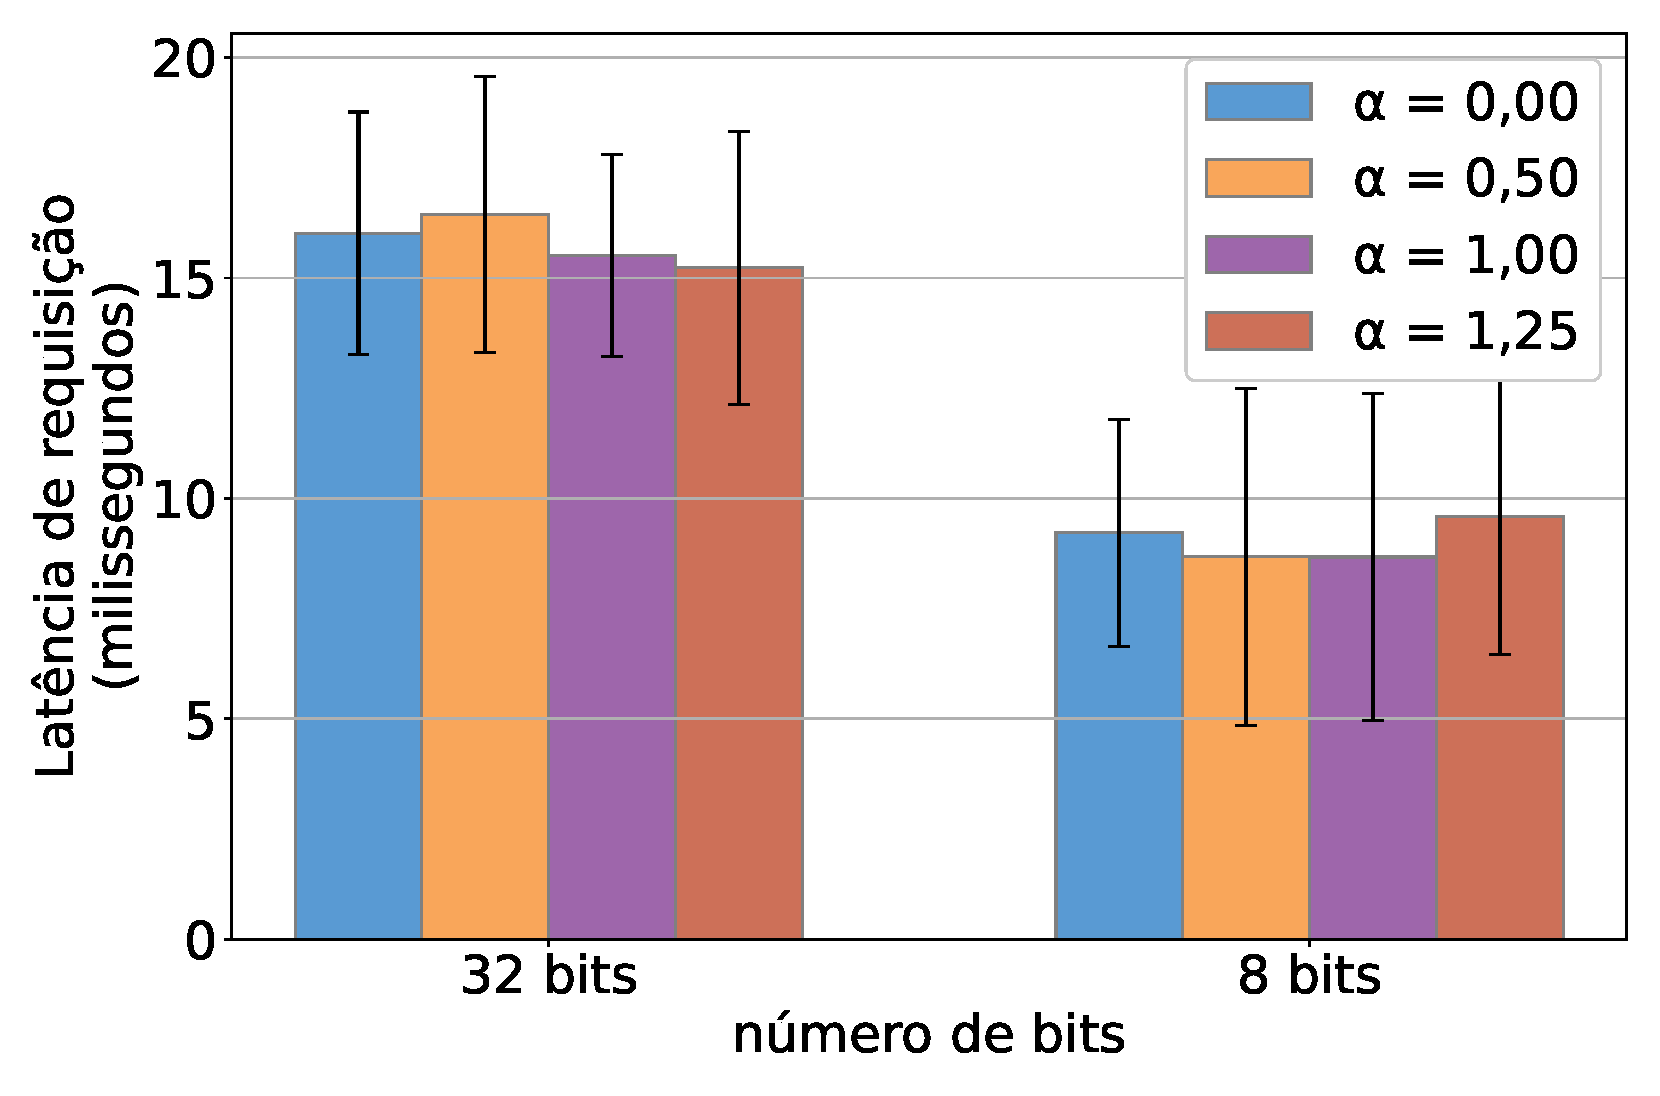
\includegraphics[width=\textwidth]{figuras/latencia2.eps}
            \caption{\scriptsize{Latências}}
          \end{subfigure}  
          \begin{subfigure}[b]{0.32\textwidth}
            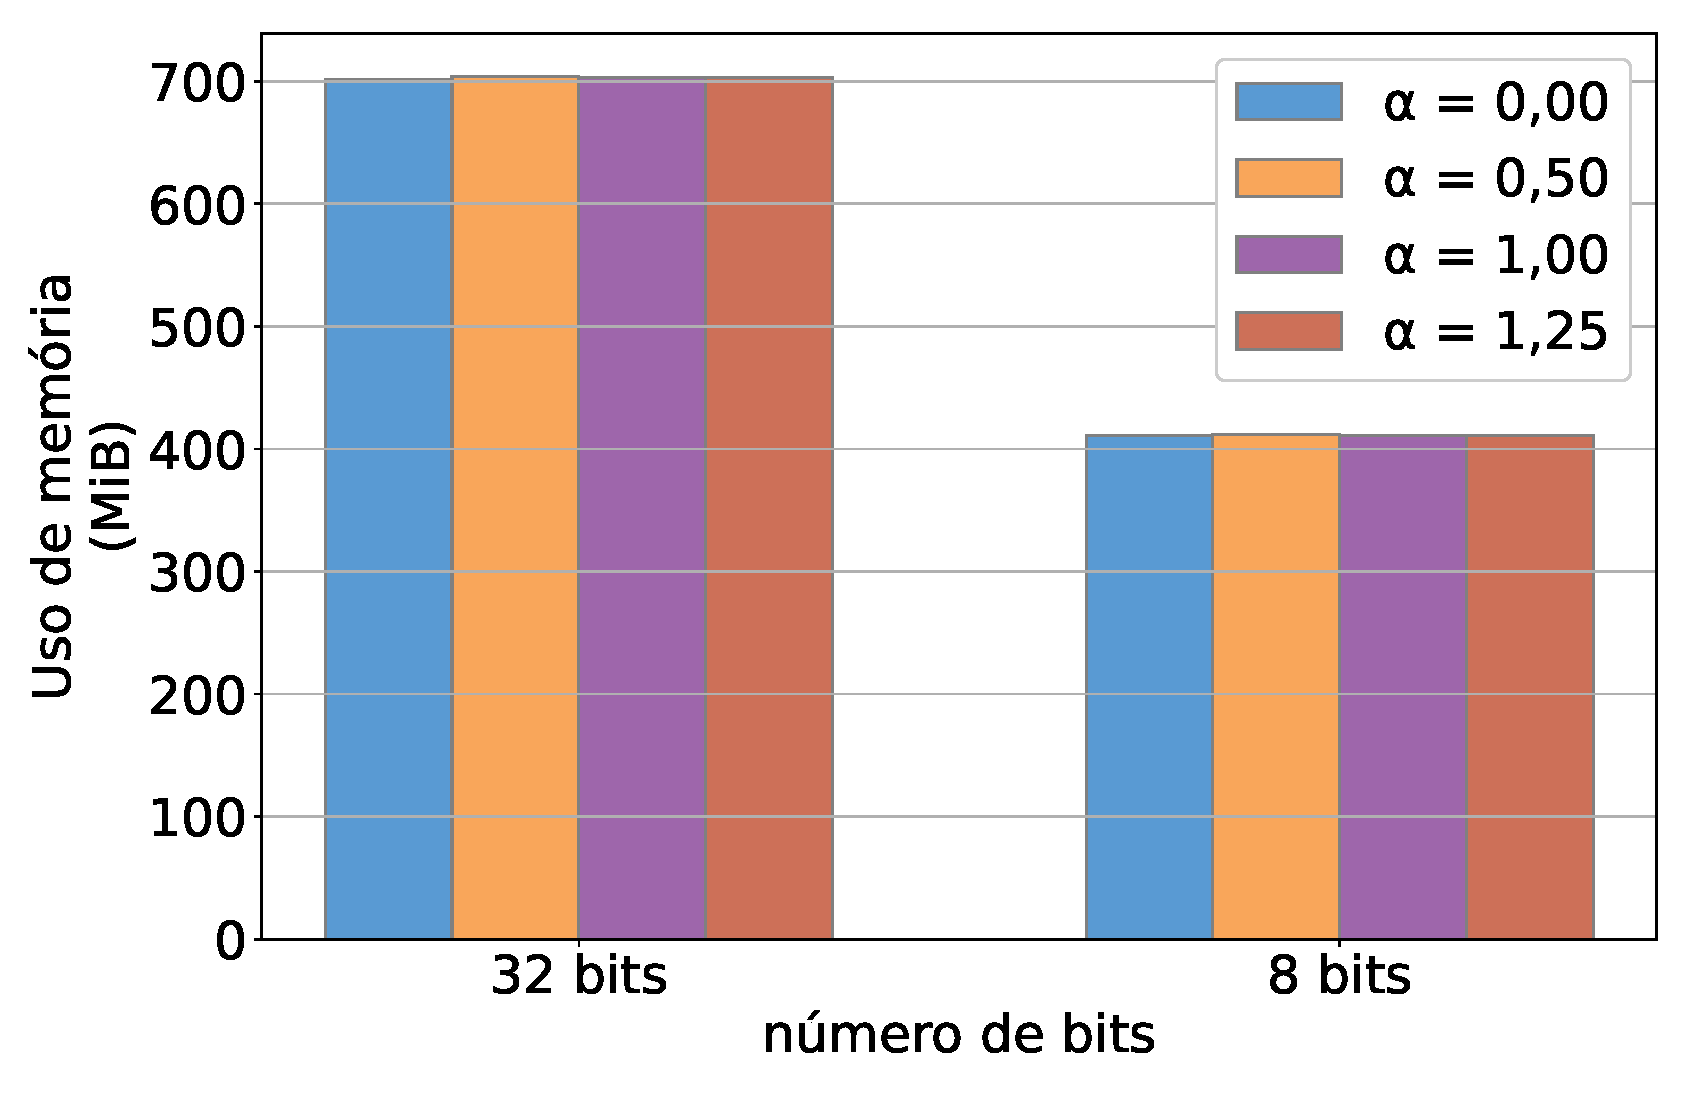
\includegraphics[width=\textwidth]{figuras/memoria2.eps}
            \caption{\scriptsize{Consumo de memória}}
        \end{subfigure}
        \begin{subfigure}[b]{0.32\textwidth}
            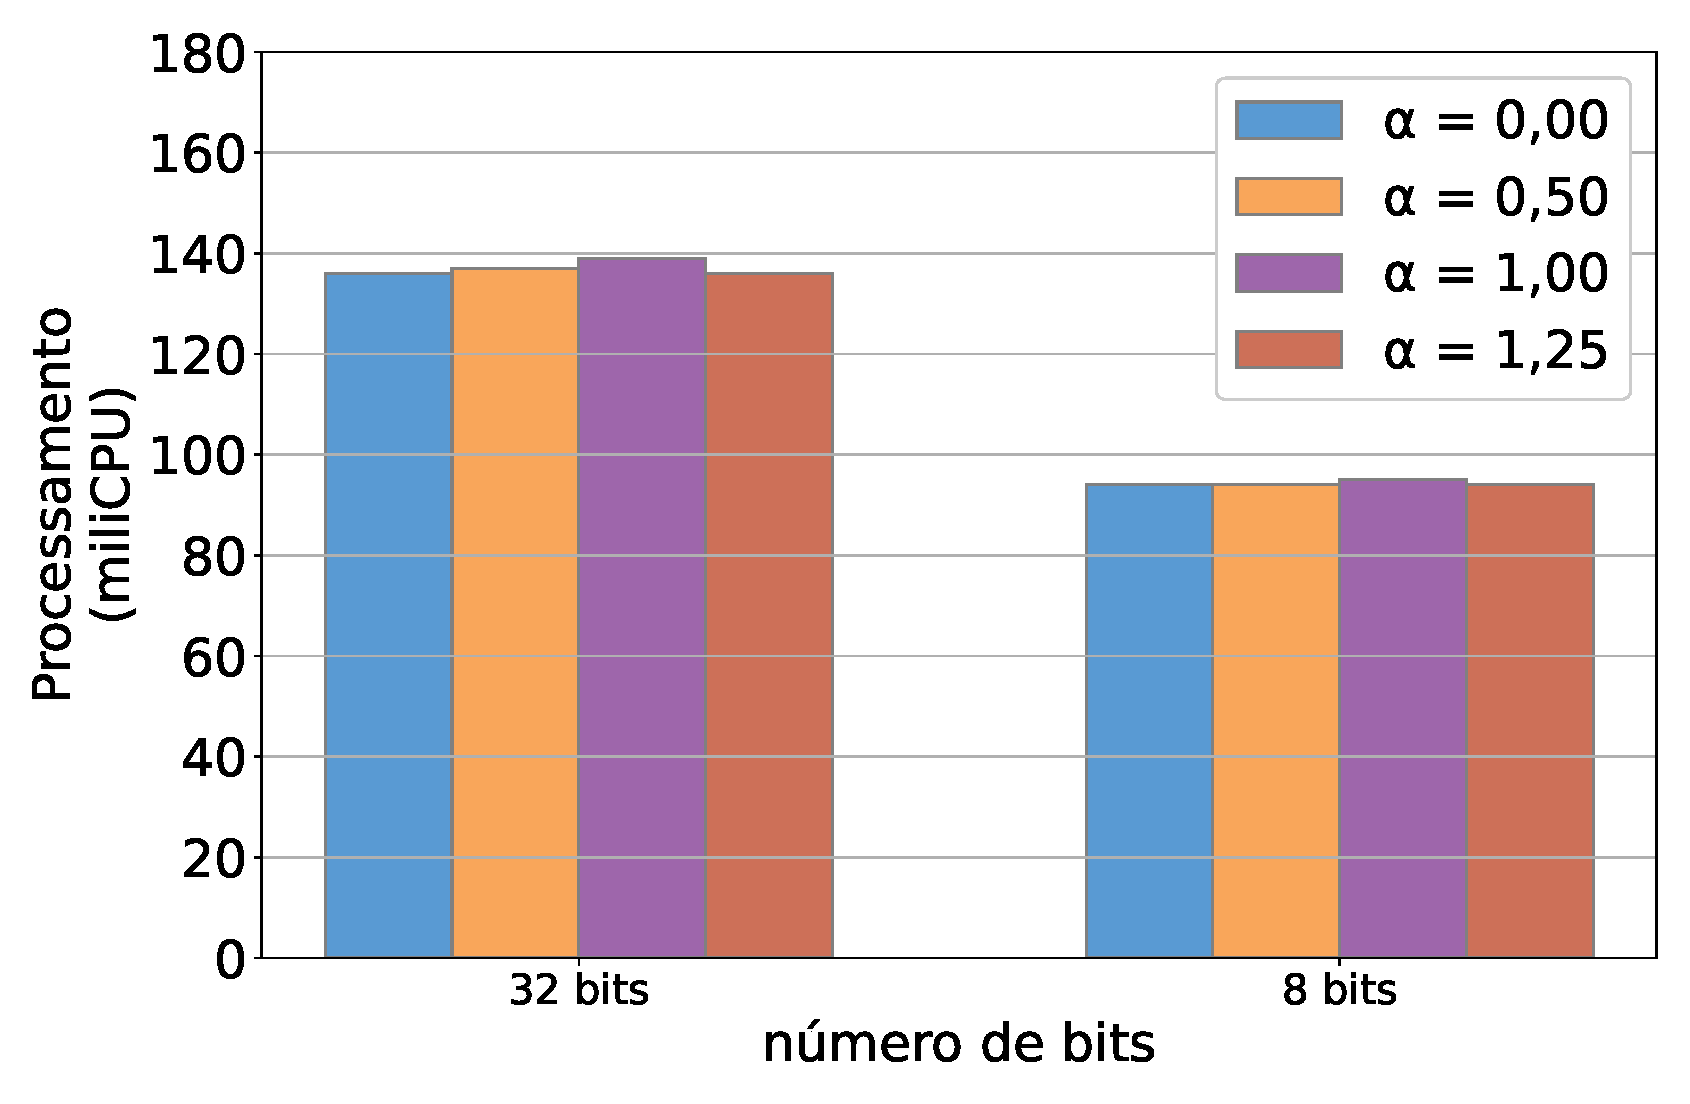
\includegraphics[width=\textwidth]{figuras/cpu2.eps}
            \caption{\scriptsize{Processamento}}
        \end{subfigure}
        \caption{\scriptsize{Latência de resposta em milissegundos, consumo de memória e uso de CPU de cada microserviço para o segundo perfil de estresse $N_2 = 125$.}}
        \end{figure}
\end{frame}

\begin{frame}{Resultados}
    \scriptsize
    \begin{table}[H]
        \caption{\scriptsize{Latência de resposta das requisições, Consumo de memória e processamento de cada microseriviço do terceiro perfil de estresse $N_3 = 250$.}}
        \centering
        \begin{tabular}{llllll} \\
        \hline
        \textbf{bits} & \textbf{$\alpha$}  &  \textbf{Latência} & \textbf{Memória} &\textbf{CPU}\\  \hline
        32 &0,00& $16,23ms \pm 3,122$ & 702MiB & 135miliCPU\\
        32 &0,50& $16,78ms \pm 3,214$ & 706MiB & 136miliCPU\\
        32 &1,00& $16,24ms \pm 3,333$ & 704MiB & 139miliCPU\\
        32 &1,25& $15,34ms \pm 2,767$ & 701MiB & 134miliCPU\\
        8  &0,00& $9,30ms \pm 2,666$ & 412MiB & 94miliCPU\\
        8  &0,50& $9,25ms \pm 2,714$ & 414MiB & 95miliCPU\\
        8  &1,00& $9,25ms \pm 2,555$ & 410MiB & 96miliCPU\\
        8  &1,25& $8,71ms \pm 2,991$ & 411MiB & 94miliCPU\\
        \hline
        \end{tabular}
        \end{table}
\end{frame}

\begin{frame}{Resultados}
    \begin{figure}[H]
        \centering
        \begin{subfigure}[b]{0.32\textwidth}
            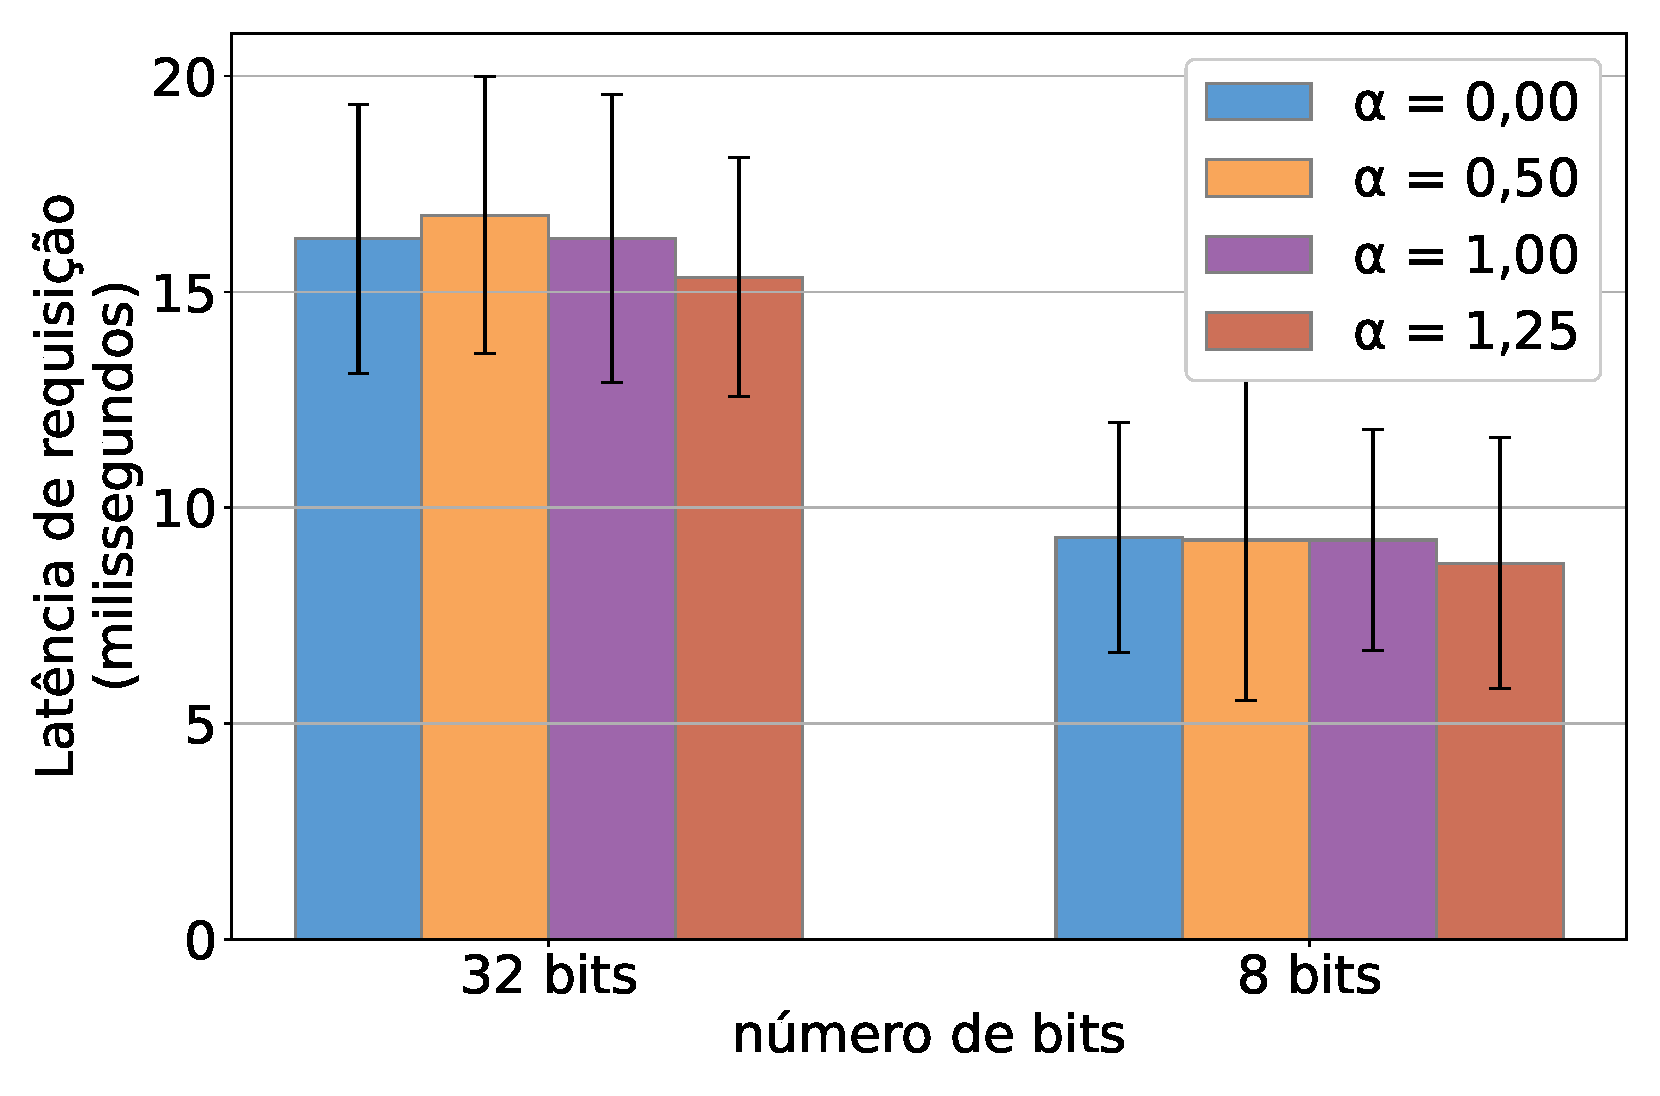
\includegraphics[width=\textwidth]{figuras/latencia3.eps}
            \caption{\scriptsize{Latências}}
          \end{subfigure}  
          \begin{subfigure}[b]{0.32\textwidth}
            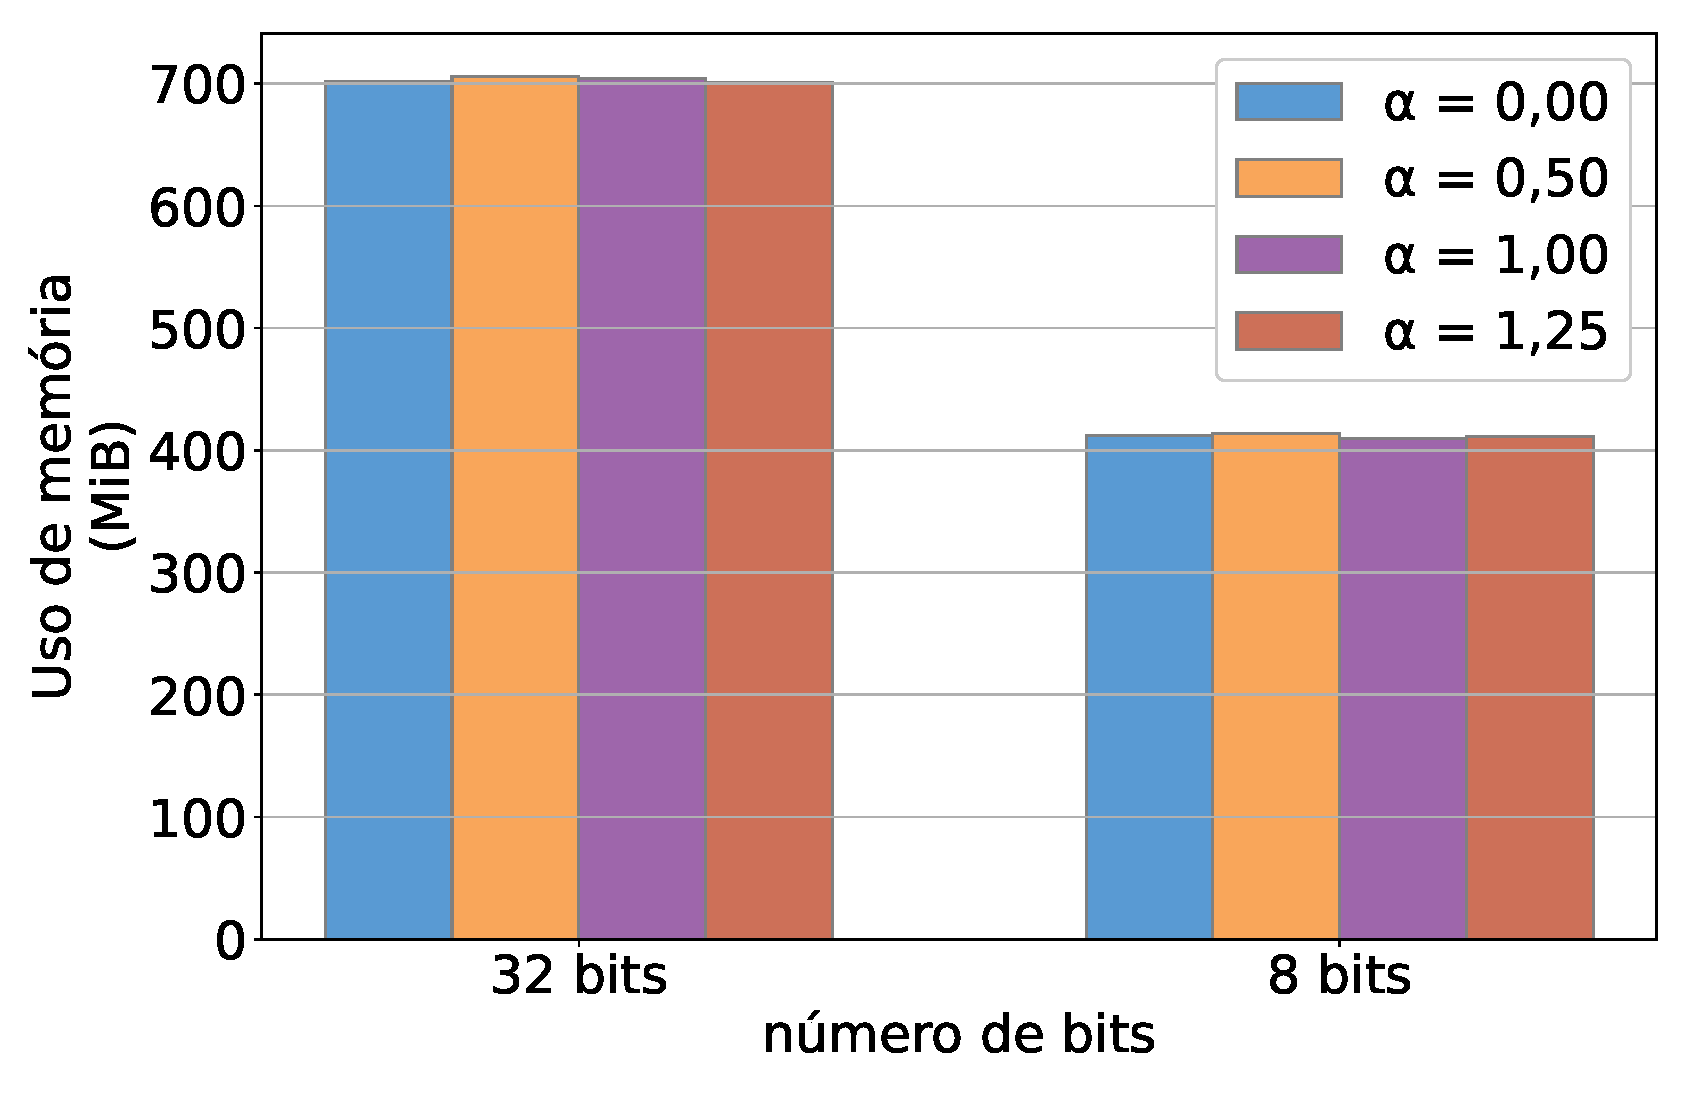
\includegraphics[width=\textwidth]{figuras/memoria3.eps}
            \caption{\scriptsize{Consumo de memória}}
        \end{subfigure}
        \begin{subfigure}[b]{0.32\textwidth}
            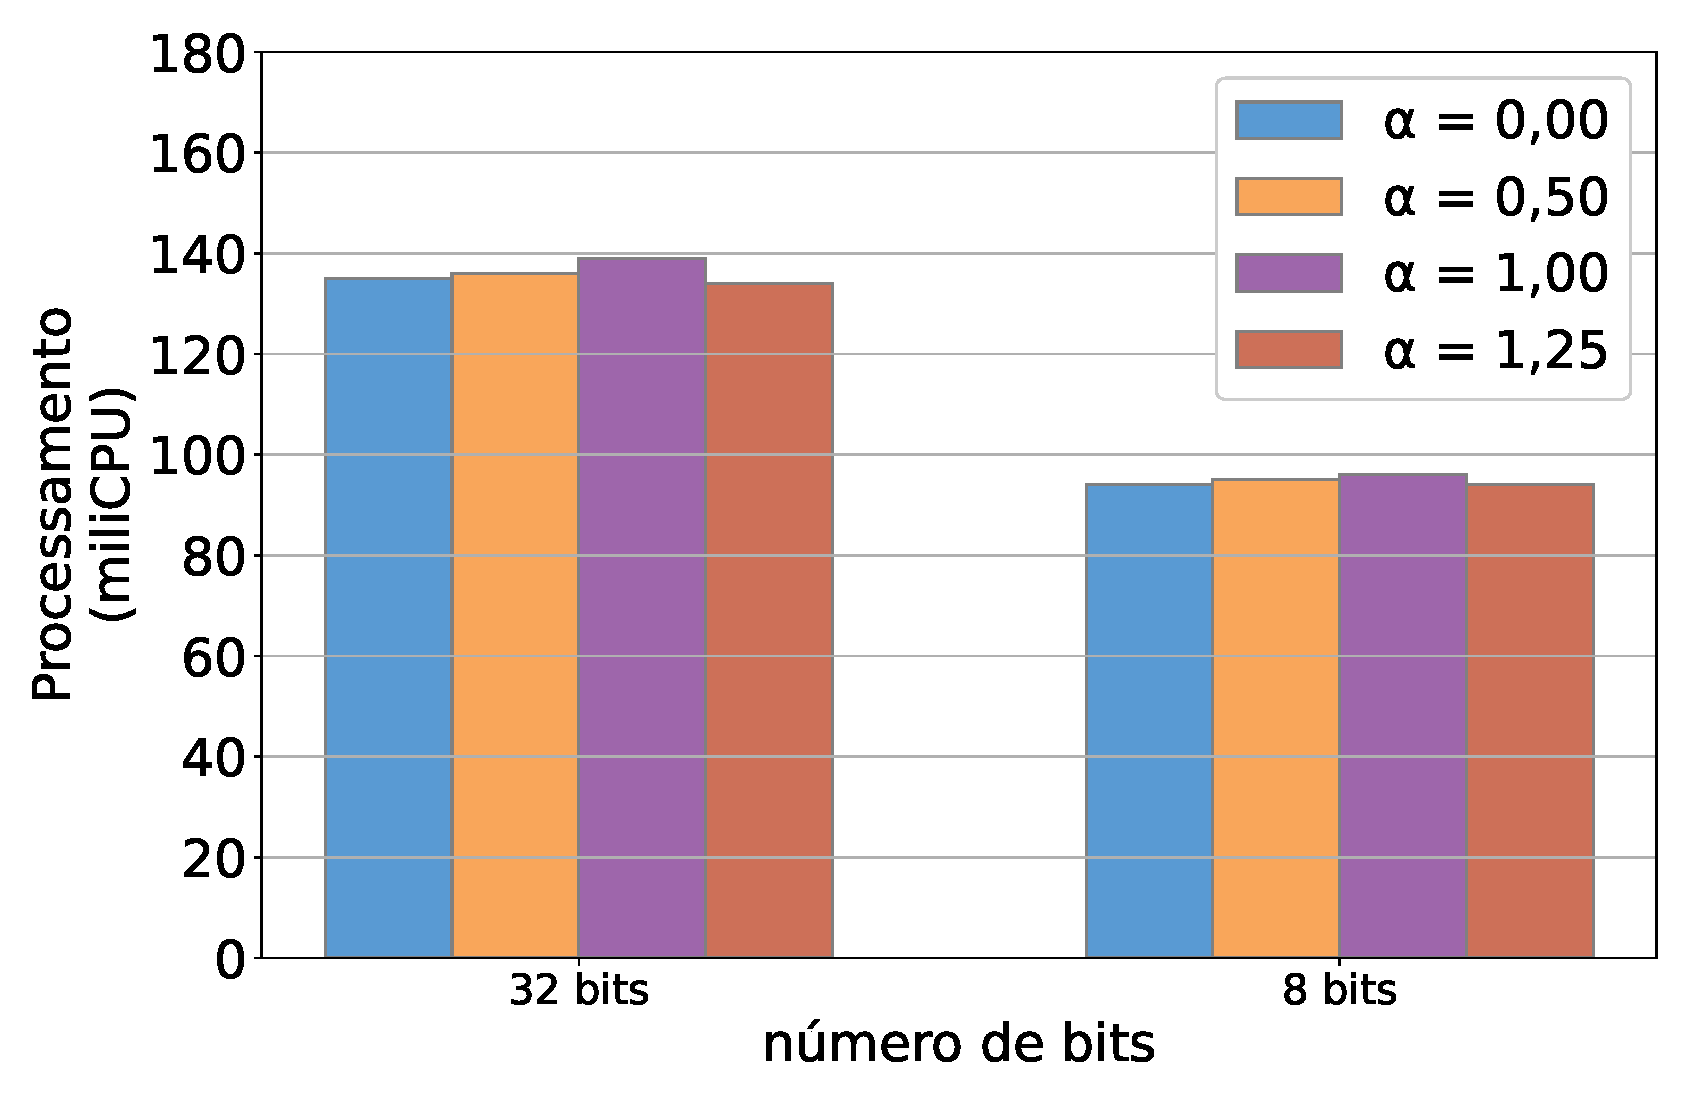
\includegraphics[width=\textwidth]{figuras/cpu3.eps}
            \caption{\scriptsize{Processamento}}
        \end{subfigure}
        \caption{\scriptsize{Latência de resposta em milissegundos, consumo de memória e uso de CPU de cada microserviço para o terceiro perfil de estresse $N_3 = 250$.}}
    \end{figure}
\end{frame}

\begin{frame}{Resultados}
    \scriptsize
    \begin{table}[H]
        \caption{\scriptsize{Tempo médio para criação de uma nova réplica.}}
        \centering
        \begin{tabular}{l|llll}
        \hline
        \textbf{\diagbox{bits}{$\alpha$}} & \textbf{0,00}  & \textbf{0,50} & \textbf{1,50} & \textbf{1,25}\\ \hline
        \textbf{32 bits} & $2,71s \pm 0,0220$ & $2,72s \pm 0,0267$ & $2,57s \pm 0,0306$ & $2,41s \pm 0,0294$\\
        \textbf{8 bits} & $2,30s \pm 0,0199$ & $2,25s \pm 0,0444$ & $2,22s \pm 0,0212$ & $2,14s \pm 0,0409$\\\hline
        \end{tabular}
    \end{table}
\end{frame}

\begin{frame}{Resultados}
    \begin{figure}[H]
        \centering
        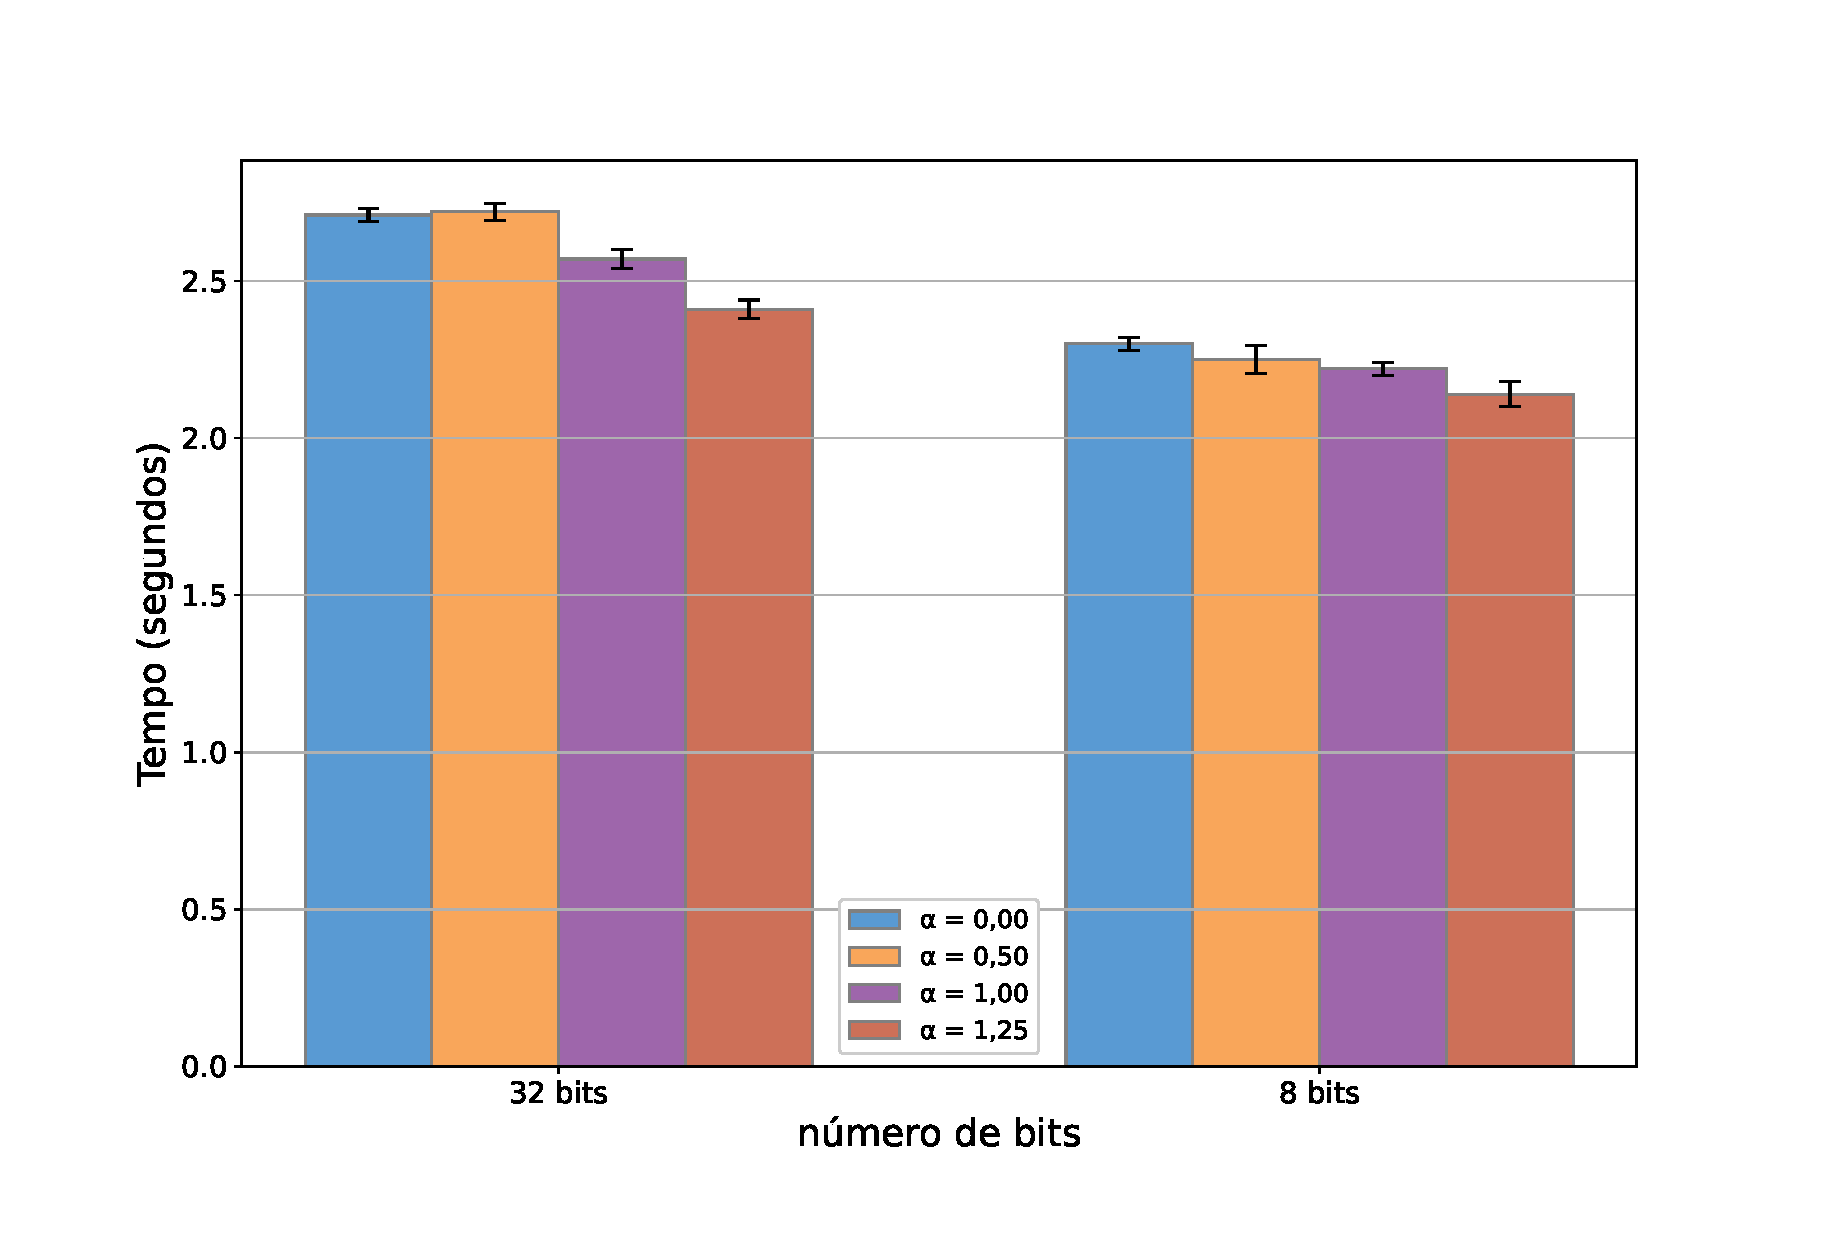
\includegraphics[width=0.7\textwidth]{figuras/hpa.eps}
        \caption{Tempo médio para criação de uma nova réplica.}
    \end{figure}
\end{frame}


\begin{frame}{Infraestrutura}
    \begin{figure}[H]
    \centering
    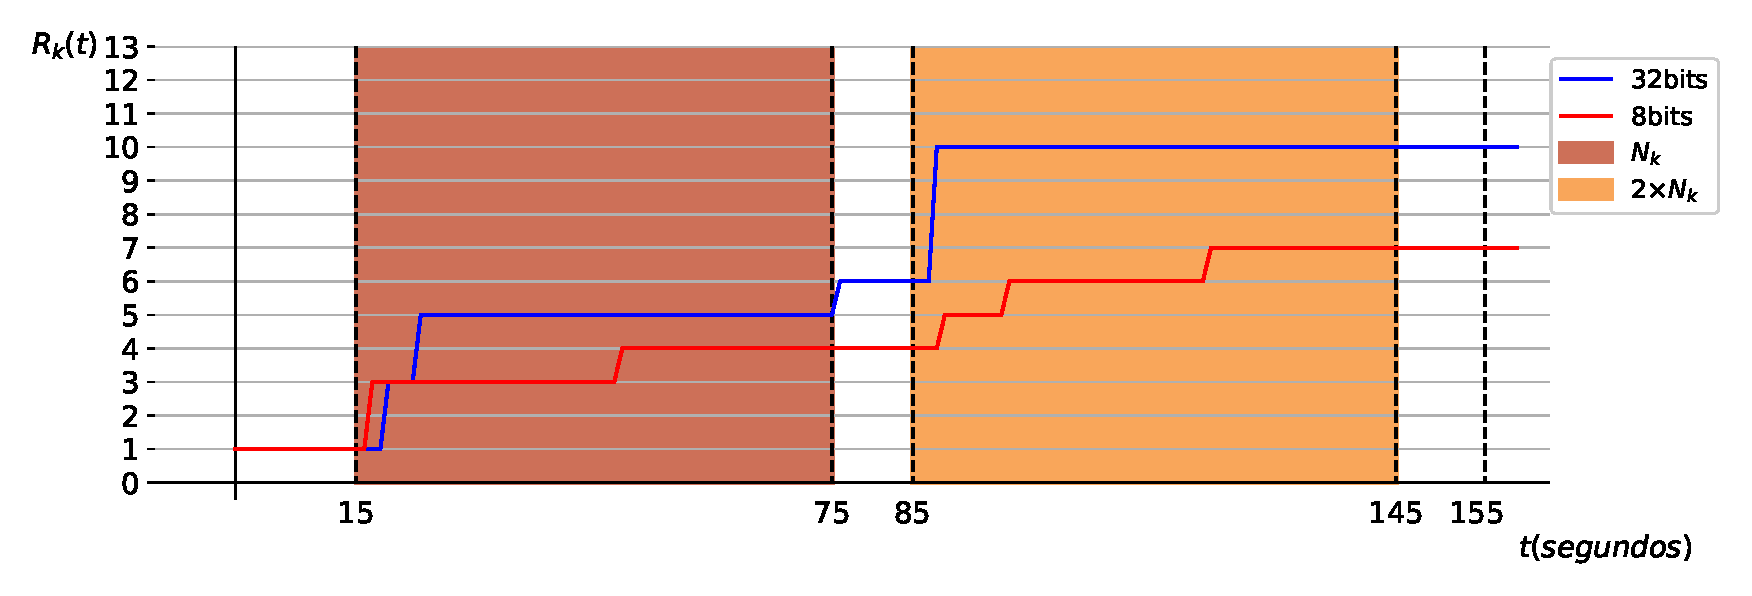
\includegraphics[width=1\textwidth]{figuras/escalonamento.eps}
    \caption{Comportamento da criação de novas réplicas com o passar do tempo do modelo não comprimido e quantizado em $8$ bits o primeiro perfil de estresse $N_1=75$.}
    \end{figure}
\end{frame}

\begin{frame}{Infraestrutura}
    \begin{figure}[H]
    \centering
    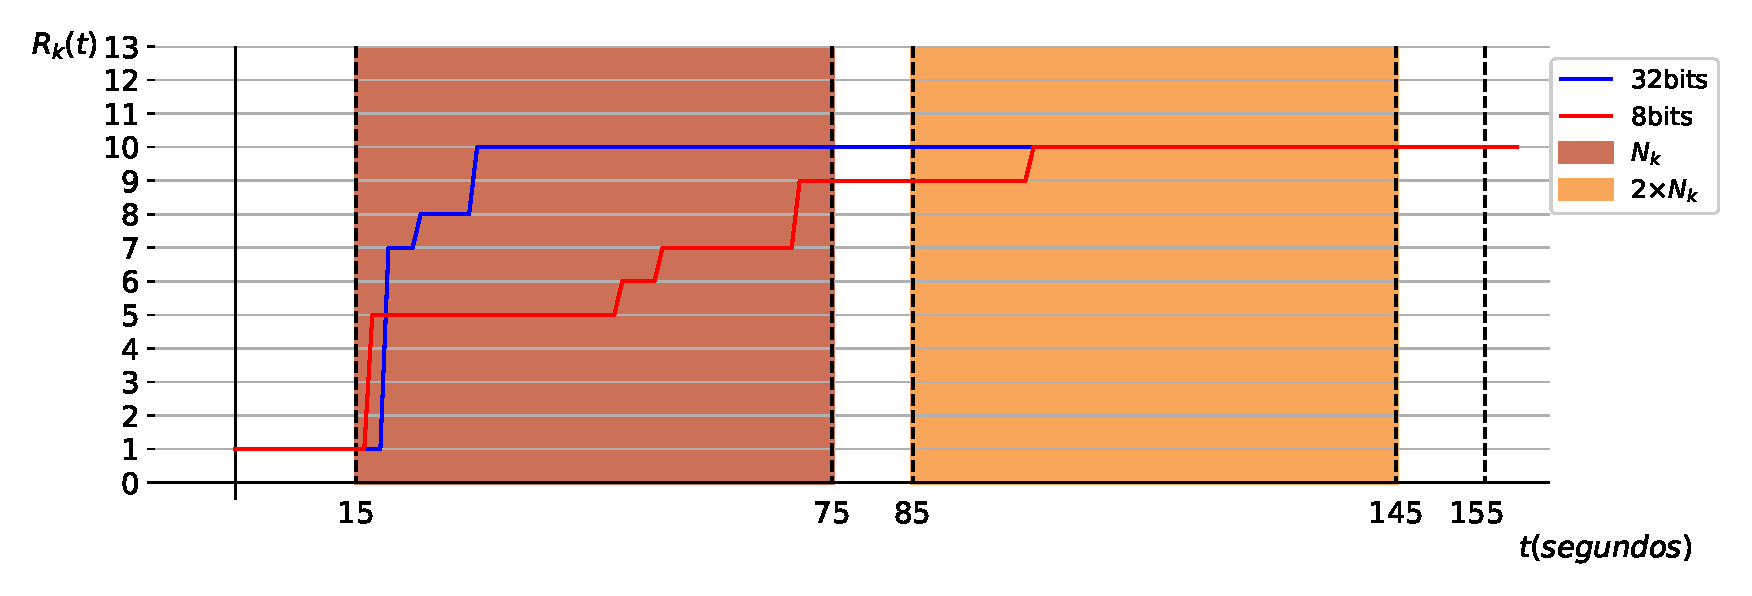
\includegraphics[width=1\textwidth]{figuras/escalonamento2.eps}
    \caption{Comportamento da criação de novas réplicas com o passar do tempo do modelo não comprimido e quantizado em $8$ bits o segundo perfil de estresse $N_2=125$.}
    \end{figure}
\end{frame}

\begin{frame}{Infraestrutura}
    \begin{figure}[H]
    \centering
    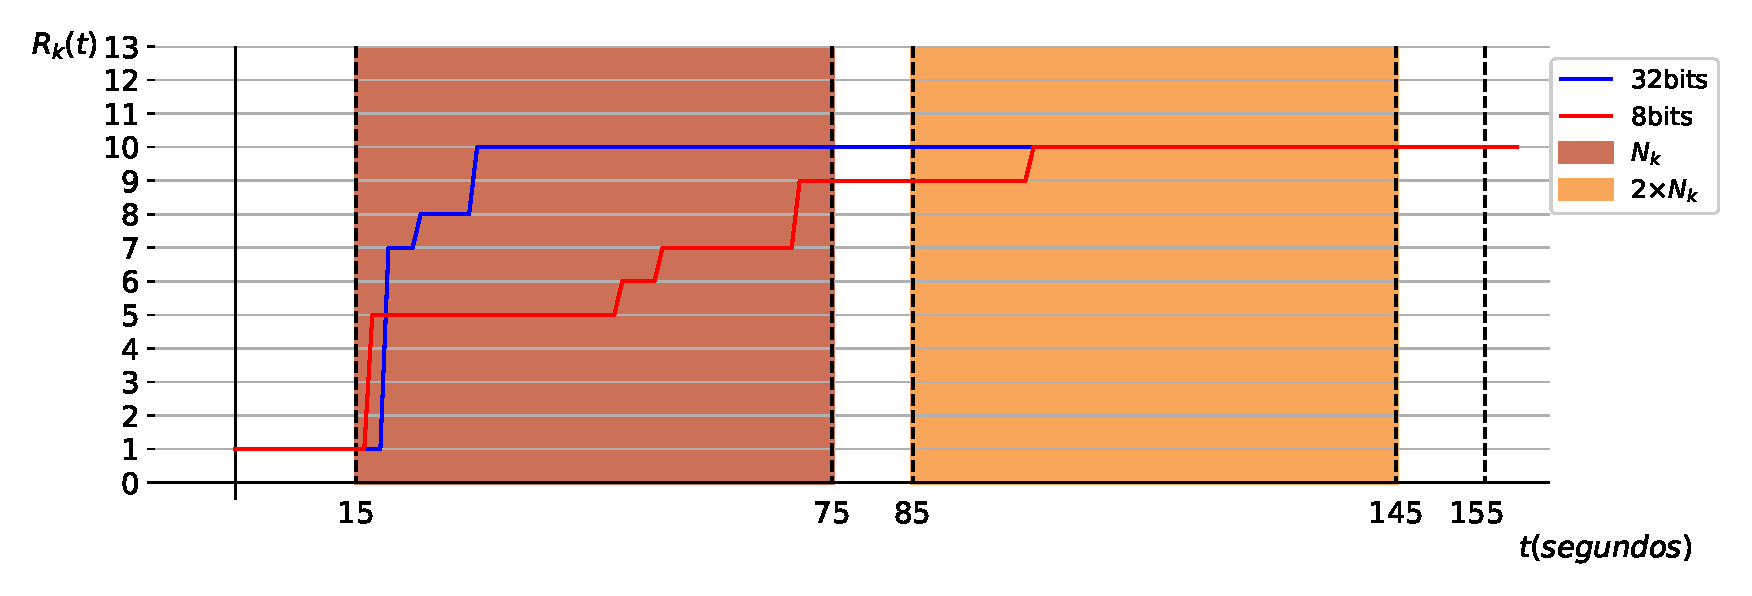
\includegraphics[width=1\textwidth]{figuras/escalonamento2.eps}
    \caption{Comportamento da criação de novas réplicas com o passar do tempo do modelo não comprimido e quantizado em $8$ bits o terceiro perfil de estresse $N_3=250$.}
    \end{figure}
\end{frame}

% Conclusao
\section{Conclusões}
\begin{frame}{Conclusões}
    \scriptsize
    \begin{itemize}
        \item A adoção das técnicas de compressão deste trabalho diminuem o tamanho do modelo sem comprometer substancialmente sua acurácia;
        \item As estratégias de compressão utilizadas são viáveis para diferentes domínios;
        \item A utilização da compressão consciente se mostrou eficaz na redução do uso de memória, processamento e latência de resposta dos modelos;
        \item A compressão de modelos se mostra benéfica para sua utilização em ambientes distribuídos (microserviços).
    \end{itemize}
\end{frame}

\begin{frame}{Trabalhos futuros}
    \scriptsize
    \begin{itemize}
        \item Utilizar outra estratégia para geração de modelo e comparar com a compressão de Deflate, como o formato esparso;
        \item Aplicar a compressão de modelos em outros domínios, como sistemas embarcados;
        \item Inclusão de novas métricas, como consumo de energia para outros domínios.
    \end{itemize}
\end{frame}

% Referencias
\section{Referencias}
\begin{frame}{Referências}
    \tiny
    \nocite{fernandes2021}
	\nocite{blalock2020}
	\nocite{nvidea2015}
    \nocite{Quantization1}
    \nocite{Quantization2}
    \nocite{PruneQuantization1}
    \nocite{Quantization4}
	\bibliography{bib/bibliografia}

\end{frame}


% Agradecimentos
\section{}
%\begin{frame}{Agradecimentos}
%	Agradeço a todos. 	
%\end{frame}

\end{document}